%\newcount\draft\draft=0 % set to 0 for "publication"
%\nonstopmode % ignore compiler errors

\documentclass{report}

\usepackage{geometry}
\usepackage{graphicx}
\usepackage{hyperref}
\usepackage{supertabular}
\usepackage{array}
\usepackage{enumitem}
\usepackage{tabularx}
\usepackage{framed}
\usepackage[usenames,dvipsnames]{color}
\usepackage{colortbl}
\usepackage[table]{xcolor}
\usepackage{lscape}
\usepackage{listings}
\usepackage{mdframed}
\usepackage{float}

\usepackage{longtable}

\usepackage[utf8]{inputenc}

\newcommand*{\Package}[1]{\texttt{#1}}%

\graphicspath{{src/figure/} }
\begin{document}

%This is the Titlepage
%%=========================================
\thispagestyle{empty}

\mbox{}\\[6pc]
\begin{center}
\Huge{IT2901 - Informatics Project II}\\[2pc]
\huge{IDI Open}\\
\huge{Programming Contest System}\\[2pc]

\Large{Haakon Konrad William Aaseb{\o}}\\
\Large{H{\aa}kon Gimnes Kaurel}\\
\Large{Tino Hakim Lazreg}\\
\Large{Filip Fjuk Egge}\\
\Large{Anders Sildnes}\\
\Large{Eirik Fosse}\\[1pc]

\large{May 2014}\\[2pc]

Norwegian University of Science and Technology
\end{center}
\vfill

\noindent Supervisor: Hong Guo

 % This is the titlepage
\setcounter{page}{0}
\pagenumbering{roman}
\section*{Foreword}
Originally inspired by the Nordic Collegiate Programming Contest (NCPC),
it has been held at NTNU every spring since 2007. The format is a
five-hour contest with competing teams consisting of one, two or three
contestants. A team of volunteer judges write the problems and answer
clarification requests during the contest, while another team hands out
balloons for each solved problem. Usually a rather hectic affair, it is
extremely important that everything is well prepared. The number of
teams is often more than 100, with the record being 162 teams in 2011

The contest system that verifies solutions is at the heart of the
contest when it is in progress, and needs to be working perfectly at
all times. The system must handle several submissions per second, while
verifying that each one is correct and runs within the set resource
limits. Submissions must show up on the high score list, and when
problems are solved the team handing out balloons must be notified. In
addition to this there were a lot of other functional requirements
having to do with the bureaucracy of organizing the contest

A requirement was that new features could be easily added in the future,
and the code was written with this in mind. The project will now become
open source, and all programming contest enthusiasts will soon be able
to request and implement their desired features

All aspects of this project have been pleasing and delightful for us.
The team has exceeded all our expectations and their system will be
used for years to come.

\hfill -- \textit{Christian Chavez, IDI Open Manager}

\pagebreak

\section*{Preface}

IT2901 is the most prestigious course for bachelor students studying
informatics. This motivated us to give the best of our self. This report is
written spring 2014 by six students at NTNU, Norwegian University of Science
and Technology, Department of Computer and Information Science, IDI. It has
been a great and educational journey. 

For the past few months, we have taught ourselves a new programming language
and framework and used advanced development tools - while tackling many social
and technical conflicts.  We’ve proven how ``Ambition is a dream with a V8
engine'', as Elvis Presley once said. 

The group would like to thank our eager customers, Christian Chavez, Finn
Inderhaug Holme and Christian Neverdal Jonassen for their time to meet us and
provide constructive feedback. We also owe a big  thanks to our friends and
family, for understanding our choice to work during easter. Big thank you to
our supervisor, Hong Guo, for constructive criticism and reflections; without
which, we would not ascertain the peak of our own potential.

\tableofcontents
\setcounter{page}{0}
\pagenumbering{arabic}
% \chapter{Introduction}
\section{About the course}
Our group and assignment has been delegated as part of the course
IT2901: ``Informatics Project II''
at NTNU. The work covers 15 course credits, equivalent to a 50\% work
position for one academic semester. IT2901 is offered only to those
that are enrolled on the NTNU's informatics BSc
programme.

The primary purpose of the course is to let students apply their
knowledge\ from other courses. This is rendered through a project for a
real customer. The students have to communicate independently with
their client, and deliver a software product that answers the
client's needs. 

Grades are based on the satisfaction of the customers and an evaluation
of the development process. The latter will be reviewed through written
reports and timesheets, as provided in this document. Furthermore, it
is important that students have met the given deadlines and documented
their work in a structured manner.

\section{The Group}

The team consists of six members. All the members of the group are
completing their BSc degree in Computer Science from NTNU in 2014. We
had prior experience working together, and knew each other well. With
many shared courses and similar interests, the team are all at a
somewhat similar level of competence. However, we have different areas
of expertise, and exploiting this has been a key to success on previous
occasions. For a detailed description of each member, see the listing
below.

\begin{description}
\item[Anders Sildnes]
Throughout his BSc, Anders has been taking courses related to algorithms
and program security. Apart from his studies, he is developing for
Engineers without Borders NTNU and spending time with open-source
projects and other Linux tools.

\item[Eirik Fosse]
Eirik has a primary interest in artificial intelligence and machine
learning. In the course of his bachelor's degree
he's focused on programming, mathematics, and
evolutionary simulation.

\item[Filip Fjuk Egge]
While achieving his degree, Filip has taken courses focused on a path
related to system development and security. He has a varied education
and knowledge\ on different aspects of computer science. 

\item[Haakon Konrad William Aaseb{\o}]
Haakon has selected disciplines related to mathematics and algorithms.
Apart from being a student at NTNU he is playing football at NTNUI in
the third division. 

\item[H{\aa}kon Gimnes Kaurel]
During his time at NTNU, H{\aa}kon has been keeping a primary focus on
courses related to programming and the intersection between hardware
and software. He's also got experience as an app
developer, and has extensive knowledge\ of the GNU/Linux operating
system. 

\item[Tino Lazreg]
Tino has been taking courses related to different aspects of software
engineering, like programming, system architecture, human-machine
interaction. Besides doing a BSc, Tino also works as a student
assistant in a human-machine interaction course on NTNU. 
\end{description}

\section{About the Customer}
Our customer is IDI Open. They are responsible for the annual
programming contest mentioned in 1.2. Christian Chavez is our main contact for
the project, but his two colleagues, Christian Neverdal Jonassen and Finn
Inderhaug Holme, were
also available for questions. They are all students of computer science
at NTNU. 

\section{About the Contest}
IDI Open is a programming contest where teams of up to three people meet
and solve programming problems of various difficulty. The contest lasts
five hours, and the objective is to solve as many problems as possible.
The contest is open for all types of programmers, from students of all
grades to professors and other professionals from the IT industry.
Various prizes are given to the teams based on their performance. There
are usually 8-12 problems in a contest. To make the competition fun for
everyone, there are typically some problems that are easy enough even
for novice programmers to handle. The main objective is to solve the
highest amount of problems in the shortest amount of time.

\section{Stakeholders}
Our stakeholder fall into two different categories: the ones involved in
the competition, and those involved in the course.
\subsection{Course}

\begin{description}
\item[Supervisor]
The supervisor's job consists of guiding and helping us
through this project. This aid was primarily focused on the development
process and the writing of this report. The supervisor tries to ensure
that the developers communicate properly and have a structured approach
to developing the end product. To verify this, we have had bi weekly
status reports delivered to the supervisor, as well as regular
meetings.

\item[Examiner]
The examiner(s) is responsible for determining our final grade. Unlike
the other stakeholders, we have not communicated with the examiner
throughout the development process. Though, the examiner has got access
to all the documents the supervisor has got access to.
\end{description}

\subsection{Product}
\begin{description}
\item[IDI Open]
The project's primary stakeholders. They are the host of
the competition in which our product was used. Their inclusion in this
product comprised all aspects of our project.

\item[Judges]
The judges are hired by IDI Open to supervise the competition, service
contestants and create problem sets. They will rely on our end product
achieve the mentioned tasks. Throughout the process they have given
feedback to our customers, IDI Open, about our product. Naturally, the
judges are important to the contest, so it is important that they are
satisfied with the software they have to use.

\item[Developers]
The developers are responsible for satisfying all other parties. Similar
to the customer, our involvement in this project is total.

\item[Maintainers]
As IDI Open is an annually recurring event, our end product, if
successful, will be used for many years in the future. At a point, we
assume the code will need to be replaced or modified. Assumably, there
will be another developer team to do this. As such, the quality of of
our product will impact them.

\item[Sponsors]
Different companies sponsor each contest. In exchange for money and
services, the sponsors get exposure through ads on the website and get
to give a short presentation during the awards ceremony. Naturally, the
sponsors want to associate their name with a successful product.
Therefore, the sponsors rely on that contests are successful - this is
heavily based on our product.

\item[Contestants]
The actions of contestants are all through our software; our product
will be their medium to take part in IDI Open. Reliability and
usability is key to keep the contestants happy. The contestants also
gave feedback to the customers about their user experience. Thus, how
satisfied the contestants are impacts the developer's
evaluation.
\end{description}

\section{Goals}
The goal of the project is to upgrade and improve the existing system
used in IDI Open. We were given sole responsibility for our project; no
other team or organization of developers has had responsibility for our
solution.This gave us inspiration to do the best we could, and to give
the customer something both we and they could be proud of for many
years to come. And if the product is good enough it would hopefully
also be used in larger programming competitions, maybe even
international ones.


% \chapter{Task Description and Overview}

\section{Task Description and Overview}
\label{sec:taskdesc}

The first step in our development process was to get a brief overview of
our complete system. To do this, we have followed a conventional style
of designing UML use cases together with a textual description. From
reading this chapter, the reader should be able to understand how our
end product works. The assumptions and constraints that affected our 
process are also discussed in section~\ref{sec:assumtions}. 
Reading this chapter will be important to
understand the rest of this report.  

\section{Assignment}
According to our customer, IDI Open's previous solution was
cumbersome to use. Our assignment was to create a replacement system
that would be easier to administer.
This included replacing both front and back-end systems.

The features of the old solution, in a nutshell, are given below.
\begin{itemize}
\item Website containing information about the contest
\item Team-registration and scoring
\item Ability for users to upload code to be compiled and executed
\end{itemize}

We were given access to the code for the old solution. The customers
felt that this code was cluttered, but we could re-use components
wherever we wanted. However, it was important that we did this in an
structured manner, such that other developers could easily understand the
new solution.

\section{GentleIDI}

Since we were delivering an end product to a real customer, we wanted to
present ourselves as a real company. We chose the name
``GentleCoding'' as our
representative name. This was used to name our repositories, email
lists and other media communicated with external parties.

The term ``Gentle'' is supposed to
represent our calm approach to problems. It is also similar to
``Gentleman'', which reminds of quality and good conduct. Furthermore, it is
easy to interpret and remember.

Since we were developing a new system, we also wanted to brand our product. We
wanted to keep it logical and simple, so we decided on ``GentleIDI''.
Consequently, GentleIDI may be used to refer to our end product throughout the
rest of the report.


\section{Assumptions and Constraints}
\label{sec:assumtions}
To define what is satisfactory, we have made some assumptions and
defined some constraints. Table~\ref{table:assumtions} should make it easier to
understand how we have reasoned our system design. 

% \begin{table}
% \caption{Assumtions and constraints}
% \label{table:assumtions}
% \tablehead{}
% \begin{supertabular}{|p{0.33\textwidth}|p{0.33\textwidth}|p{0.33\textwidth}|}
% \hline
\begin{longtable}{|p{.33\textwidth}|p{.33\textwidth}|p{.33\textwidth}|}
\caption[test]{Assumtions and constraints} \\
\hline \multicolumn{1}{|c|}{\textbf{Assumption/Constraint}} &
\multicolumn{1}{c|}{\textbf{Why}} &
\multicolumn{1}{c|}{\textbf{Implication}} \\
\hline 
\endfirsthead

\multicolumn{3}{c}%
{{\bfseries \tablename\ \thetable{} -- continued from previous page}} \\
\hline \multicolumn{1}{|c|}{\textbf{Assumption/Constraint}} &
\multicolumn{1}{c|}{\textbf{Why}} &
\multicolumn{1}{c|}{\textbf{Implication}} \\
\hline 
\endhead
Assumption/Constraint & Why & Implication\\\hline The system will be maintained
by people who have experience with computers. & People that are involved with
any programming contest are typically programmers themselves. & User design,
words and definitions can be made more technical. Error messages can be
explained using computer lingo. \\\hline

The system will be used and maintained for {\textgreater} 5 years &
Customer-constraint: they do not want to spend too much time
developing new products, so maintenance is preferred. & The code should be
written in a modular, extensible way with clear documentation.\\\hline

The customer is based at Gløshaugen. & & High availability for customer
meetings and reviews.\\\hline

The developers will maintain a 20 hour a week work ethic throughout the
project{}-duration of 20 weeks[TODO: update]. & To finish the product on time.
& The set of requirements should not require more than 20 hours of work per
week per developer, in order to complete.\\\hline
Our system should be user{}-friendly &
Our solution features a web interface available to everyone. Ideally,
any person should be comfortable with the user interface. &
Should have a user{}-friendly interface.
\\\hline
Our end product will be open sourced. &
To ensure quality, and let other volunteers contribute to the code
repository. &
No proprietary third party modules can be used. \ We cannot copyright
our own material. \\\hline
The final product must run on Linux{}-computers. &
This is the choice of OS by NTNU, which is responsible for technical
support and server access. &
Linux{}-compliant solution.\\\hline
We are allowed to use whatever third party plugin we want, as long as it
is free and has no copyright{}-conflict. &
Speed up development. &
Speed up development.\\\hline
\end{longtable}

Do note that the implications in table~\ref{table:assumtions} were not necessarily upheld.
Rather, they were used as initial bounds to permit leeway. For example,
imposing that third party plugins will speed up development does not
mean that we would alway prioritize software re-use.

\section{Roles and Their Definitions}
\subsection{Usergroups}
Within the application-domain of
GentleIDI there are different
groups of users. Each group has different levels of access control, and
once a user is made a member of that group, they inherit those rights.
A user may have membership in all groups. A privileged user is someone
who is given elevated permissions. Table~\ref{table:usegroup} shows the
different roles and their available actions. Further elaborations on
each group will also be given in later sections, but table~\ref{table:usegroup} should
suffice for an overview.

\begin{longtable}{|p{.2\textwidth}|p{.6\textwidth}|}
\caption{Usergroup overview} \label{table:usegroup}\\
\hline
\multicolumn{1}{|c|}{\textbf{ID}} &
\multicolumn{1}{c|}{\textbf{Story}} \\
\hline
Role &
Description\\\hline
Admin &
Privileged. An admin can modify all the available settings of the
system\\\hline
Judge &
Privileged. Similar to an admin account, but with a limited set of
actions: answering questions (clarification system), upload problem to be
solved, solutions to those problems, and incorrect answers (e.g.\ answers
that will provide penalty).\\\hline
Functionary &
Privileged. Functionaries hand out balloons when a team has solved a
problem. To determine what team will be given a balloon, the functionaries
have their own interface with a team overview.\\\hline
Contestants &
A contestant has an account on the system and has the possibility to
enter and compete in a contest. \\\hline
Team &
A group of one to three contestants. A contestant is only part of one
team per contest, and need a team in order to compete. \\\hline

\end{longtable}

\subsection{Service-providing Units}

Another way of viewing the task description in section~\ref{sec:taskdesc}, is to say
that our solution needs to do three actions: serve web-content, store
data and execute user-submitted code. Since each of these operates with
different protocols, we will think to our solution as composed of three
different systems. These are described in figure X.X. 

\begin{longtable}{|l|m{0.5\textwidth}|m{0.2\textwidth}|}
\caption{Service-providing Units} \label{table:serviceUnits} \\
\hline
\hline \multicolumn{1}{|c|}{\textbf{Entity}} &
\multicolumn{1}{c|}{\textbf{Features}} &
\multicolumn{1}{c|}{\textbf{Protocol}} \\
\hline
Webserver & Processes requests from contestants and teams. Also acts as an
interface to the execution node, both receiving and transmitting data
to other execution nodes on the behalf of users. & HTTP\\\hline

Execution node & A service, often on a dedicated platform, that offers the
ability to compile and execute code. The execution node returns output data to
the webserver. & AMQP\\\hline

Database & The storage unit for all user{}-data and logs. & SQL\\\hline
\end{longtable}



\section{UML Use Cases}
We need one page each for privileged, registered, and non-registered
users. That is, one interface for administrative users, one for
contestants, and one for non-registered viewers. From each of these
three, we defined use case scenarios. Figure X.X and X.X models the
available workflows and actions for each category of users.
Table~\ref{table:uml-notation} describes the semantics of objects used in the
diagram, which should be equivalent to the UML 2.0 standard.
\begin{longtable}{|m{0.15\textwidth}|m{0.7\textwidth}|}
\caption{UML Notation} \label{table:uml-notation} \\
\hline
	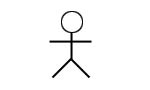
\includegraphics[width=0.15\textwidth]{chapter2-img1.jpg}  &
Use case actor. Represents a user group\\\hline
	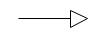
\includegraphics[width=0.15\textwidth]{chapter2-img2.png}  &
UML generalization arrow. Used to indicate inheritance. The
arrow's tail represents the entity that
inherits from where the arrow points to.\\\hline
{\textless}{\textless}include{\textgreater}{\textgreater} &
UML stereotype to represent a mandatory extension to a
workflow.\\\hline
{\textless}{\textless}extend{\textgreater}{\textgreater} &
UML stereotype to indicate that if certain conditions are met in a flow,
the entity to which this arrow points to can extend the
workflow.\\\hline
\end{longtable}

The purpose of the use case diagrams is to give a clear overview of what
users shall be able to accomplish from our system. Furthermore, use
case diagrams are easier to communicate to external parties, such that
it is easier to agree on the system's properties. The
use case diagrams were used early in development to agree on the
requirements specification and to communicate what we
were trying to accomplish.

\begin{figure}[h!]
    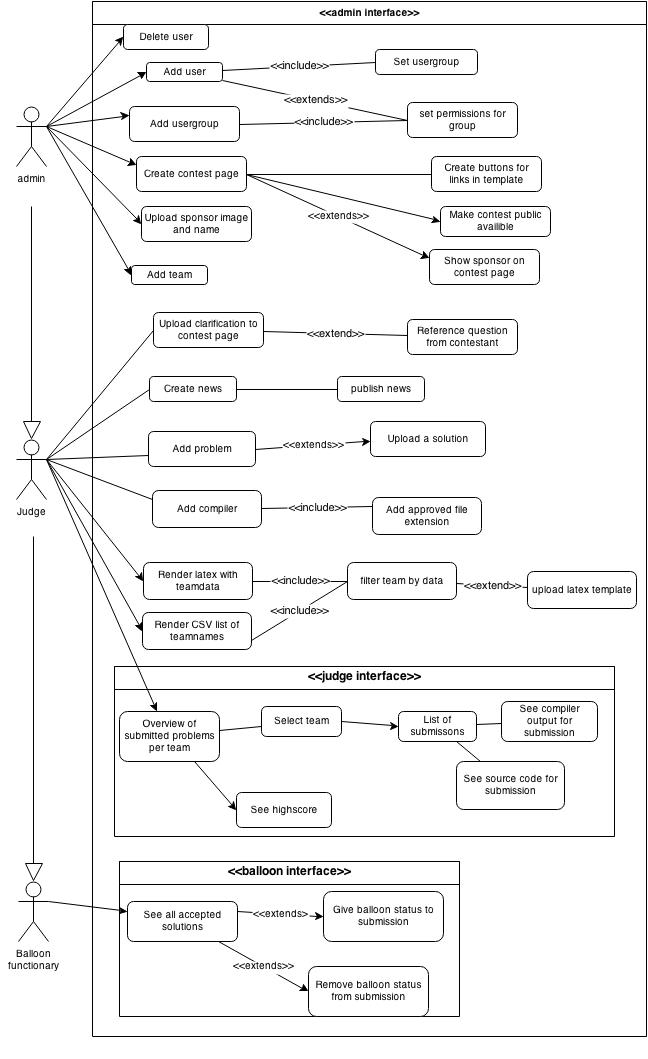
\includegraphics[width=0.8\textwidth]{chapter2-img3.jpg}
    \caption{FIGURECAPTION} \label{figure:usecase}
\end{figure}
As seen in figure~\ref{figure:usecase}, admins has privileges to perform the
actions of any other group, in addition to their own set of actions. Thus,
membership in the admin group gives a user complete control in the application
domain. Furtherly, it can be noted that all usergroups have the opportunity to
act as a contestant to review the website.  Privileged users will are still
restricted from appearing in the official high score tables to prevent them
from assuming a competing role. This was to avoid the chance of any person with
access to the solutions to compete.

% \chapter{Project Management}
This chapter will go through the different project roles we deemed
important. We will explain our development method, which tools we use
and give an overview of how we planned the project. Furthermore, in
section~\ref{section:WBS}. We also provide a structured overview of how we organized
our time. 

\section{Project Roles}
We wanted to ensure that all developers had an even workload and
experience in all components of our project. We
maintained a flat organizational structure where all decisions were
made in groups. No member would work alone on a task for a longer
period of time. Some tasks and delegations were easier to assign only once.

The most central role is that of the scrum master. The role mainly
consists of setting up meeting agendas and keeping control of what
team members are working on. In addition, the scrum master should act
as a buffer between the team and other distractions. The scrum master had a
casting vote whenever there was a disagreement. The group elected Haakon to be
scrum master because of his well established authority and organization.

We also assigned the role of a transcriptionist. His job consists of
writing a short summary of every meeting, and making this available to
the rest of the group. This includes meetings with the customer and
supervisor. This job was performed by Anders, who volunteered for the
position. We assigned Håkon to be customer contact, and
Tino as responsible for room reservations.

\section{Development Method (Scrum)}
Scrum focuses on having daily meetings, and constantly adjusting to
changes by iterative development. This makes it easier to predict and
to adjust for problems that may occur. It was hard to predict what
would happen in our project, therefore our sprints were short, lasting
at most two weeks. The transition between two sprints was done during a
prolonged meeting on Wednesdays. During this meeting we evaluated the
latest sprint and planned the upcoming one. Every team member were
requested to say three good things and three bad things regarding the
last sprint. This was followed by a discussion of how to plan the next
sprint better. Lastly we showed what had been completed, to the other
members of the group, before setting up the next sprint. Scrum also
focuses on having finished versions of the systems on each iteration,
and to finish all packages in the given iteration.
In order to take advantage of the best in everyone's
abilities we worked in pairs where this was efficient. Working in pairs
is common in agile development. This was to improve code quality and
reduce errors.
%\footnote{[Page 2}
%href{http://www.cs.pomona.edu/classes/cs121/supp/williams\_prpgm.pdf}{http}

\section{Tools/Framework}
The customer wanted our end product to be easy to maintain for future
developers. Therefore we have chosen tools that are well known and easy
to learn. Some of the most important are:

\begin{itemize}
    \item Django, a framework written in Python.
    \item VIM and Eclipse for editing
    \item Google Drive and latex for documentation
    \item Git as version control, with github as hosting service
    \item Email lists, IRC and Facebook for communication
    \item Bootstrap and Grappelli for user interface design
\end{itemize}
A lot of different tools were considered for this system. A full list of all
tools and frameworks used and considered can be viewed in appendix
\textit{Tools and Frameworks.}

\section{Project-Level Planning}
After our initial requirements elicitation we began to plan our
development process. The purpose of the plan was to verify that we had
enough time to complete the requirements, and to avoid unforeseen
risks. This section will present the various components we introduced
to structurize the project.

\subsection{Work Breakdown Structure}\label{section:WBS}
WBS is a decomposition of the project into phases, deliverables and work
packages. Each package was further broken down into different tasks.
The benefits from the WBS are as follows:
\begin{itemize}
    \item Planning out the entire process prevents bottlenecks
    \item Clearly defining the scope of a package prevents excess or
        insufficient time usage
    \item It is easy for supervisors and other parties to evaluate and
        understand our process
\end{itemize}

Table~\ref{table:WBS} shows the work breakdown structure created. These high-level
packages were later broken down into activities, which are in the
product backlog, see appendix~\ref{appendix:productBacklog}

\renewcommand{\labelenumii}{\theenumii}
\renewcommand{\theenumii}{\theenumi.\arabic{enumii}.}
\scriptsize
\begin{longtable}{|p{.8\textwidth}|}
    \caption[test]{Work breakdown structure} \label{table:WBS} \\
\hline
\begin{enumerate}[nosep]
    \itemsep0em 
        \item Project management
        \begin{enumerate}[nosep]
    \itemsep0em 
            \item Write timesheet template
            \item Look at the reflection notes
            \item Meetings
            \begin{enumerate}[label*=\arabic*.]
    \itemsep0em 
                \item Internal
                \item Customer
                \item supervisor
            \end{enumerate}
            \item  Report
            \begin{enumerate}[label*=\arabic*.]
    \itemsep0em 
                \item Preliminary version
                \item Mid-semester version
                \item Final version
            \end{enumerate}
            \item Risk assessment
            \item WBS
            \item Status report
            \item Activity plans
        \end{enumerate}

        \item Pre-study        
        \begin{enumerate}[nosep]
    \itemsep0em 
            \item Install and learn tools
            \item Learn language/framework
            \item Course
        \end{enumerate}
        \item Design
            \begin{enumerate}[nosep]
    \itemsep0em 
            \item Requirement Specification
            \begin{enumerate}[label*=\arabic*.]
    \itemsep0em 
                \item Functional
                \item Non-functional
            \end{enumerate}
            \item  System architecture
            \item Database modeling
            \item User Interface
                \begin{enumerate}[label*=\arabic*.]
    \itemsep0em 
                \item Prototyping
                \item Usability Testing
            \end{enumerate}
            \item  Admin interface
        \end{enumerate}

        \item Development
        \begin{enumerate}[nosep]
    \itemsep0em 
            \item  Backend
            \begin{enumerate}[label*=\arabic*.]
                \item Execution-node(s)
                    \begin{enumerate}[label*=\arabic*.]
                    \itemsep0em 
                    \item Web-page
                \end{enumerate}
            \end{enumerate}
            \item User management
            \begin{enumerate}[label*=\arabic*.]
                \itemsep0em 
                \item User
                \item Usergroups
                \item Team management
            \end{enumerate}
            \item  Statistics
            \item Contest management 
            \item Clarification system
            \item Balloons system
            \item Unit testing
        \end{enumerate}

        \item Testing
        \begin{enumerate}[nosep]
    \itemsep0em 
            \item  User-test
            \item System-test  
            \item Final test
        \end{enumerate}

        \item Implementation
        \begin{enumerate}[nosep]
    \itemsep0em 
            \item  Deploy to production
            \item Installation
            \item Turn in to stakeholder
        \end{enumerate}

        \item Implementation
        \begin{enumerate}[nosep]
    \itemsep0em 
            \item Verify
            \item Document
        \end{enumerate}
    \end{enumerate} \\
\hline
\end{longtable}
\normalsize

We also created a gantt chart. Here, each package was assigned an
estimated time period, over how long time we expected to use. For ease
of comprehension, not every package was included from the WBS.\ The
gantt chart is shown in figure~\ref{gantt}
\newline
\begin{longtable}{|l|l|l|l|l|l|l|l|l|l|l|l|l|l|l|l|}
\caption{Gantt chart} \label{gantt} \\
\hline
\textbf{WP Name} & 1 & 2 & 3 & 4 & 5 & 6 & 7 & 8 & 9 & 10 & 11 & 12 & 13 & 14 & 15 \\
\hline
Project management & \cellcolor{ForestGreen} &\cellcolor{ForestGreen}&\cellcolor{ForestGreen}&\cellcolor{ForestGreen}&\cellcolor{ForestGreen}&\cellcolor{ForestGreen}&\cellcolor{ForestGreen}&\cellcolor{ForestGreen}&\cellcolor{ForestGreen}&\cellcolor{ForestGreen}&\cellcolor{ForestGreen}&\cellcolor{ForestGreen}&\cellcolor{ForestGreen}&\cellcolor{ForestGreen}&\cellcolor{ForestGreen} \\
\hline
WBS &\cellcolor{YellowGreen}&\cellcolor{YellowGreen}&&&&&&&&&&&&& \\
\hline
Pre-study
&\cellcolor{yellow}&\cellcolor{yellow}&\cellcolor{yellow}&\cellcolor{yellow}&&&&&&&&&&&
\\ \hline
Install and learn tools&\cellcolor{Dandelion}&\cellcolor{Dandelion}&\cellcolor{Dandelion}&\cellcolor{Dandelion}&&&&&&&&&&& \\
\hline
Learn language/framework&&\cellcolor{Dandelion}&\cellcolor{Dandelion}&\cellcolor{Dandelion}&&&&&&&&&&&  \\
\hline
Course &&\cellcolor{Dandelion}&\cellcolor{Dandelion}&&&&&&&&&&&&  \\
\hline
\textbf{Design} & &\cellcolor{MidnightBlue} &\cellcolor{MidnightBlue} &\cellcolor{MidnightBlue} &\cellcolor{MidnightBlue} &\cellcolor{MidnightBlue} &\cellcolor{MidnightBlue} &\cellcolor{MidnightBlue} &\cellcolor{MidnightBlue} &\cellcolor{MidnightBlue} & & & & & \\ \hline
Requirement specification&&\cellcolor{RoyalBlue}&\cellcolor{RoyalBlue}&\cellcolor{RoyalBlue}&\cellcolor{RoyalBlue}&\cellcolor{RoyalBlue}&\cellcolor{RoyalBlue}&\cellcolor{RoyalBlue}&\cellcolor{RoyalBlue}&\cellcolor{RoyalBlue}&&&&&  \\
\hline
System architecture&&&\cellcolor{RoyalBlue}&\cellcolor{RoyalBlue}&\cellcolor{RoyalBlue}&\cellcolor{RoyalBlue}&\cellcolor{RoyalBlue}&&&&&&&&  \\
\hline
Database modelling&&&\cellcolor{RoyalBlue}&\cellcolor{RoyalBlue}&\cellcolor{RoyalBlue}&\cellcolor{RoyalBlue}&&&&&&&&&  \\
\hline
Tests &&&\cellcolor{RoyalBlue}&\cellcolor{RoyalBlue}&\cellcolor{RoyalBlue}&\cellcolor{RoyalBlue}&&&&&&&&&  \\
\hline
User-interface&&&&&\cellcolor{MidnightBlue}&\cellcolor{MidnightBlue}&\cellcolor{MidnightBlue}&\cellcolor{MidnightBlue}&\cellcolor{MidnightBlue}&&&&&&  \\
\hline
\textbf{Development}&&&&\cellcolor{Purple}&\cellcolor{Purple}&\cellcolor{Purple}&\cellcolor{Purple}&\cellcolor{Purple}&\cellcolor{Purple}&\cellcolor{Purple}&\cellcolor{Purple}&&&&  \\
\hline
Execution node&&&&&&&&\cellcolor{Orchid}&\cellcolor{Orchid}&\cellcolor{Orchid}&\cellcolor{Orchid}&&&&  \\
\hline
Implement single node&&&&&&&&\cellcolor{Thistle}&\cellcolor{Thistle}&\cellcolor{Thistle}&&&&&  \\
\hline
Implement several nodes&&&&&&&&&\cellcolor{Thistle}&\cellcolor{Thistle}&&&&&  \\
\hline
Content Management System&&&&&&&&&&&\cellcolor{Orchid}&&&&  \\
\hline
Front end&&&&\cellcolor{Orchid}&\cellcolor{Orchid}&\cellcolor{Orchid}&\cellcolor{Orchid}&\cellcolor{Orchid}&\cellcolor{Orchid}&\cellcolor{Orchid}&\cellcolor{Orchid}&&&&  \\
\hline
\textbf{Testing}&&&&&&&\cellcolor{Red}&\cellcolor{Red}&\cellcolor{Red}&\cellcolor{Red}&\cellcolor{Red}&\cellcolor{Red}&\cellcolor{Red}&\cellcolor{Red}&\cellcolor{Red}  \\
\hline
Unit testing &&&&&&&\cellcolor{Orchid}&\cellcolor{Orchid}&\cellcolor{Orchid}&\cellcolor{Orchid}&\cellcolor{Orchid}&\cellcolor{Orchid}&\cellcolor{Orchid}&\cellcolor{Orchid}&\cellcolor{Orchid}  \\
\hline
Integration testing&&&&&&&&&\cellcolor{Melon}&\cellcolor{Melon}&\cellcolor{Melon}&\cellcolor{Melon}&\cellcolor{Melon}&\cellcolor{Melon}&\cellcolor{Melon}  \\
\hline
System test&&&&&&&&&\cellcolor{Melon}&\cellcolor{Melon}&\cellcolor{Melon}&\cellcolor{Melon}&\cellcolor{Melon}&\cellcolor{Melon}&\cellcolor{Melon}  \\
\hline
\textbf{Production}&&&&&&&&&&&&&&\cellcolor{MidnightBlue}&\cellcolor{MidnightBlue}  \\
\hline
Post-implementation&&&&&&&&&&&&&&&\cellcolor{Plum} \\
\hline
\end{longtable}

The gantt chart was revised several times during the first four sprints,
mainly due to new deadlines set by the customer. 

\pagebreak
\subsection{Milestones}
Throughout the project, the supervisor, customer, and the project group set
deadlines. Some of the milestones marks the completion of work packages. We
have four of these milestones, M-03, M-05, M-06 and M-07. The other milestones
represents events with deadlines that were given by the course stakeholders.
These are M-01, M-02, M-04, M-08. The group used the milestones in order
to determine if the project is on schedule and to monitor the progress.
The reader can view what requirements that were met for each milestone
in~\ref{section:functionalreq}.

\begin{longtable}{|l|p{1.3cm}|p{1.3cm}|p{1.3cm}|p{1.3cm}|p{1.3cm}|p{1.3cm}|p{1.3cm}|p{1.3cm}|}
    \caption{Milestone name and deadlines} \label{table:milestone} \\
\hline

Date & 09.02. & 09.03. & 19.03. & 19.03. & 11.04. & 26.04. & 03.05. & 30.05.\\
\hline

Week & 3 & 6 & 8 & 8 & 11 & 14 & 15 & 18\\
\hline

Name & Prelimin- ary report & Mid-semester report & First release &
Presen- tation & Beta release & IDI Open test event & IDI \ Open & Final Report\\
\hline

ID & M-01 & M-02 & M-03 & M-04 & M-05 & M-06 & M-07 & M-08\\
\hline
\end{longtable}



\begin{description}
    \item[Preliminary report M-01]
    Preliminary report is the delivery of the first version of the report.
    This was to help us get started with important aspects of the project work.

    \item[Mid-semester report M-02]
    This version of the report should present all of the analysis and most of
    the design of our system. The delivery date for the mid-semester report
    is 16th of March. We wanted to complete this one week earlier, 9th of March,
    focus on M-03.

    \item[First release M-03]
    This milestone marks the groups first delivery to the customer. In summary
    this release should make it possible for contestants to sign up for a
    competition. Three days prior to the release the group will meet up with
    the customer and overlook that all the requirements are met. This meeting
    will also act as an introduction on how to manage the system.

    \item[Presentation M-04]
    The main purpose of the presentation is for the class to share their
    experiences and learn from other groups. 

    \item[Beta-release M-05]
    The beta release should contain most of the essential features. This
    version of the program should only be a release to a selected group of
    people. 

    \item[IDI Open test event M-06]
    On April 26th there will be a test event where everybody could test the
    system. This means that leading up to this event the system should be a
    release candidate. 

    \item[IDI Open M-07]
    This is the day of the competition and the system should be a release
    version. 

    \item[Final report M-08]
    This milestone marks the final date for delivering the report and the end
    of our project. Based on feedback received from the competition the group
    might choose to implement some changes to the system. 
\end{description}

\subsection{Meetings}
Our meetings can be categorized in three categories: internal, supervisor and
customer meeting. We established some meetings rules:
\begin{itemize}
    \item All meetings follow ``the academic quarter'', meaning that the time
        of start was XX:15
    \item Members that were late had to bring a cake to the next meeting
    \item All members may at any time propose a coffee break, a proposal that
        has to be followed. 
    \item No laptop should be open during the meetings
\end{itemize}

\subsubsection{Internal Meetings}
We had three internal meetings each week. Two of which were daily scrum
meetings. These were primarily set to be on Mondays and Thursdays.
During these meetings each group member would answer three questions: 
\begin{itemize}
    \item What have you done since the last meeting?
    \item What are you planning to do until the next meeting?
    \item Do you have any problems regarding the completion of your task? 
\end{itemize}
The group would usually continue to work together after these meetings. 

On Wednesday we had longer meetings marking the end of one sprint and
the beginning of the next. This meeting would consist of a sprint
review meeting and a sprint retrospective, where we discussed
\begin{itemize}
    \item What was good/bad with the last sprint?
    \item What should we try to improve during the next sprint?
\end{itemize}
After that we held a sprint planning meeting and created a new sprint
backlog. Our official meeting structure for this meeting can be viewed in the
appendix~\ref{appendix:endOfMeeting}

\subsubsection{Supervisor Meeting}
Meetings with the supervisor was generally held at a biweekly basis.
During these meetings we talked about what we had done, what we were
going to do and received feedback on what we had done. Before each
meeting we had to deliver status reports and activity charts. These
activity diagrams were early on replaced by sprint backlog and burndown
charts to facilitate the development process. 

\subsubsection{Customer Meeting}
Customer meetings were held whenever we felt that a certain part of the
requirements specification was unclear to us, and when we wanted approval of a
newly completed feature. Throughout the semester there were a lot of meetings.
As we never decided upon a fixed interval between customer meetings, the
frequency varied a lot. The couple of days leading up to a release date often
contained customer meetings in order to get everything right before starting on
the next release. During our periods of focusing on writing this report, the
frequency of these meetings naturally went down as the product did not
progress, and as a consequence we had little to discuss with the customer. 

\subsection{Resources}
This section contains the available resources for the project. We
intended to use a minimum of 20/25 hours per person each week, but
prepared for more work as we approached the deadline. This estimate was
later scaled up to a minimum of 25/30 two weeks before easter. During
easter, the amount of hours per week scaled up higher. 

\subsubsection{Planned Work}
Table~\ref{table:sprintoverview} shows our first initial draft of sprints. 

\begin{longtable}{|l|l|l|l|}
\caption{Initial sprint overview} \label{table:sprintoverview} \\
\hline
 Sprint & Range (week) & Days &
 Hours\\\hline
 1 & 3 - 4 & 7 & 15\\\hline
 2 & 4 - 5 & 7 & 20\\\hline
 3 & 5 - 6 & 7 & 20 \\\hline
 4 & 6 - 7 & 7 & 20 \\\hline
 5 & 7 - 8 & 7 & 20\\\hline
 6 & 8 - 9 & 7 & 20\\\hline
 7 & 9 - 10 & 7 & 20\\\hline
 8 & 10 - 11 & 7 & 20\\\hline
 9 & 11 -12 & 7 & 20\\\hline
 10 & 12 -13 & 7 & 20\\\hline
 11 & 13 - 14 & 7 & 20\\\hline
 12 & 14 - 15 & 9 & 33\\\hline
 Easter & 15 - 17 & 12 & {}-\\\hline
 13 & 17 - 18 & 7 & 35\\\hline
 14 & 18 - 19 (Leading up to event) & 9 & 35\\\hline
 After & 19 - 22 & 21 & 50\\\hline
 Total: & & 91 & 368\\\hline
\end{longtable}


\pagebreak
\subsubsection{Actual Work}
Table~\ref{table:actualWork} shows the actual sprints and work done. The hours
are for each person, during that sprint.
\begin{longtable}{|l|l|l|l|}
\caption{Actual work} \label{table:actualWork} \\
\hline
 Sprint & Week & Days & Hours \\\hline
 1 & 3-4 & 7 & 15\\\hline
 2 & 4-5  & 7  & 15\\\hline
 3 & 5-6 & 7  & 20\\\hline
 4 & 6-7 & 7 & 20\\\hline
 5 & 7-8 & 7 & 27\\\hline
 6 & 8-9  & 7  & 31\\\hline
 7 & 10-11 & 7  & 35\\\hline
 8 & 11-12 & 7 & 30\\\hline
 9 & 12-13 & 7  & 30\\\hline
 10 & 14-15 & 9 & 40\\\hline
 11 & 15-17 \ (starting 16.04, ending 26.04, easter) & 10 & 90\\\hline
 12 & 18-19 & 6 & 35\\\hline
 After & 19-22 & 21 & 65\\\hline
 Total & & 100 & 453\\\hline
\end{longtable}

% \chapter{Requirements Specification}
According to the gantt chart (Fig 4.1) the team were supposed to update the
requirement specification starting from week 2 and continuing up until week
10. For us it was still the case that there were a clearly identifiable
requirement specifications phase. This was primarily from week 2 up to and
including week 4. The outcome from this three week process was heavily used in
order to establish agreement between us and the customer. This chapter
presents the result from this process. 

\section{Purpose and Scope of this Specification}
The purpose of the requirement specification document is to specify the
objectives for our end product. Requirements are written at different
levels of detail. This is to make it easy to communicate the requirements to
both business and technical parties. We have mainly written the functional
requirements as stories and then broken them into smaller pieces. This makes
the requirements easy to communicate to the customer, and succinct for the
developers. These stories can be viewed in appendix~\ref{appendix:userstories}. It is important to
recognize that our project only lasted for a few months. Thus, late changes
to requirements were inserted promptly and without revision control. This is
a common practice in agile development\footnote{\ Page 91, Sommersville}.
The advantage and reason we chose not to perform revision control, is that we
could save time in not formally documenting all changes.

The coverage of the requirements is intended to be a complete coverage
of the product. This implies that all features available from the
application domain is listed in our specification. What the requirements
specification does not cover are organizational and external requirements. This
follows from the small amount of administrative users and developers involved,
and trust between the customer and the developers.

\section{Process of the Requirement Specification}
The customer passed on an initial list of requirements to our group. After a
classification and organization of the features, we drafted scenarios and
internally discussed the implication to each requested feature. Therein, we saw
what features would be infeasible and additional features we would want to
introduce to the customer. The modified list of requirements was then presented
to the customer, before proceeding with the implementation of the end-product.
Throughout the entire development process both we and the customer have been
modifying the list of requirements.

\section{Product/service Description}
In this section, you will find our interpretation of the physical user-domain.
The reader should note that some members of our group has competed earlier,
which has given us helpful empirical insight.

\subsection{Expected Physical Environment}
Our solution is used in different contexts. Table X.X has the different
application and user-domains.

\begin{tabular}{|m{3.1712599in}|m{3.1712599in}|}
\hline
IDI Open is hosted in P15, Høgskoleringen 3, on
Gløshaugen campus every year. Every team participating in the
contest get allocated their own computer. &
For offsite contestants, javascript must be enabled.\\
\hline
Software is required. A web server(Apache, Nginx), database
server(MySQL, PostgreSQL), Python with PyPi package manager.
 &
Linux kernel with ssh enabled, supplemented with a root user.
\\\hline
\end{tabular}

\subsection{User Characteristics}
Table X.X show different stereotypes of expected typical users. While open to
deviations from the stereotypes, they highlight important properties required
for our solution.

\begin{tabular}{|m{2.9837599in}|m{3.1087599in}|}
\hline
\begin{itemize}
    \item Irresponsive interfaces
    \item Incorrect data
\end{itemize}
\begin{itemize}
    \item User submission system
    \item Response types
\end{itemize}
 &
\begin{itemize}
    \item Irresponsive interfaces
    \item Node failures
    \item Incorrect data
\end{itemize}

\begin{itemize}
\item Backend system\item 
Dataflow
\end{itemize}
\\\hline
keep track of score
\begin{itemize}
\item Irresponsive interfaces
\item
Lack of overview
\end{itemize}
\begin{itemize}
\item Backend system
\item 
Dataflow
\end{itemize}
 &
\begin{itemize}
\item Dissatisfied contestants\item
No overview\end{itemize}
\begin{itemize}
\item Nothing special\end{itemize}
\\\hline
and information
\begin{itemize}
\item Mis-information
\end{itemize}
\begin{itemize}
\item Scoreboards, about competition
\end{itemize}
 &
\\
\hline
\end{tabular}

It can be seen in table X.X that the most prominent trait of our users is that
they have a background in computer science. As a consequence, it is assumed a
higher level of technical competence from our users. The user profiles also
highlight that some features were more important than others, e.g.\
responsiveness over aesthetics.

\section{Requirements}
Stories can be ambiguous and open for misinterpretation.\
we felt that a natural language specification of requirements would make it
easier to understand our application domain. To reduce miscommunication we made
sure to give each specification as short, succinct sentences. The stories were
used as a way to communicate with the customer about requirements without them
having to read through the table of requirements.

There are three different states for priorities, HIGH, MED and LOW.\
This ensured strict priorities.
Using more states would make it hard to differentiate between the priorities we
gave the requirements.

The following definitions make out the guideline for
prioritizing the requirements:
\begin{itemize}
    \item HIGH: The requirement is a ``must have''. To have a successfull product,
        the requirement must be implemented.
    \item MED: The requirement is a ``should have''. The fulfillment of the
        requirement will benefit the quality system.
    \item LOW: The requirement is a ``nice to have''. This includes functionality
        not critical to the system.
\end{itemize}

\subsection{Functional}\label{section:functionalreq}
The functional requirements are broken down in different categories.
Each category corresponds to a user group. The categories are Admin, Judge,
Contestant, Functionary, Teams, and Other. Each category has an ID, priority
and story. Table X.X shows the complete list of the requirements, while the
corresponding stories are given in appendix\ref{appendix:userstories}

The ID system can be interpreted in the following way
\begin{itemize}
    \item The F stands for Functional
    \item The second letter determines which category, e.g A stands for admin.
\end{itemize}

The milestone show when each requirement needs to be met.

\subsection{Functional requirements for Admin}
% \begin{longtable}{|p{2cm}|l|m{0.33795986in}|m{1.2684599in}|m{0.5254598in}|m{1.0983598in}|m{1.0566599in}|}
\begin{longtable}{|p{4cm}|l|l|p{4cm}|l|l|}
\caption[Feasible triples for a highly variable Grid]{Feasible triples for 
highly variable Grid, MLMMH.} \label{grid_mlmmh} \\

\hline \multicolumn{1}{|c|}{\textbf{Requrement}} &
\multicolumn{1}{c|}{\textbf{ID}} &
\multicolumn{1}{c|}{\textbf{Story}} &
\multicolumn{1}{c|}{\textbf{Comment}} &
\multicolumn{1}{c|}{\textbf{Priority}} &
\multicolumn{1}{c|}{\textbf{Milestone}} \\ 
\hline 
\endfirsthead

\multicolumn{3}{c}%
{{\bfseries \tablename\ \thetable{} -- continued from previous page}} \\
\hline \multicolumn{1}{|c|}{\textbf{Requrement}} &
\multicolumn{1}{c|}{\textbf{ID}} &
\multicolumn{1}{c|}{\textbf{Story}} &
\multicolumn{1}{c|}{\textbf{Comment}} &
\multicolumn{1}{c|}{\textbf{Priority}} &
\multicolumn{1}{c|}{\textbf{Milestone}} \\ 
\hline 
\endhead

An admin shall be able to create a new contest & FA-01 & SA-1 & A new contest
equals a new web page & HIGH & M-03 \\
\hline

An admin can choose whether the site should be published immediately or not &
FA-02 & SA-1 & & MED & M-03 \\
\hline

An admin can add custom CSS to the web-page & FA-03 & SA-1 & & LOW & M-03 \\
\hline

An admin shall be able to choose settings for the contest & FA-04 & SA-1 & of
contestants, maximum number of contestants per team, date, name.  Default
settings will be provided & HIGH & M-06 \\
\hline

An admin shall have access to all modules in the program & FA-05 & SA-2 & &
HIGH & M-06 \\ 
\hline

An admin can change permission of a usergroup & FA-06 & SA-2 & & LOW & M-06 \\
\hline

An admin can remove/add to a user group. & FA-07 & SA-2 & This
includes promoting new admins & LOW & M-06 \\ 
\hline 

An admin can deactivate users & FA-08 & SA-2 & & LOW & M-06 \\ 
\hline

An admin can remove users from the database & FA-09 & SA-2 && HIGH & M-06 \\ 
\hline

An admin can add a node & FA-10 & SA-4 & The node must be a privileged
user & HIGH & M-06 \\ 
\hline 

An admin can remove a node & FA-11 & SA-4 & & HIGH & M-06 \\ 
\hline 

An admin can manage a node. & FA-12 & SA-4 & This requirement is in terms of
compiler profiles support & HIGH & M-06 \\ 
\hline 

An admin can add more than one node & FA-13 & SA-4 & & MED & M-06 \\ 
\hline 

An admin can add news items & FA-14 & SA-5 & & HIGH & M-03 \\ 
\hline

An admin can remove new items & FA-15 & SA-5 & & MED & M-03 \\ 
\hline 

An admin can modify news item & FA-16 & SA-5 & & MED & M-03 \\ 
\hline 
\end{longtable}

\subsection{Functional requirements for Judge}
\begin{longtable}{|p{4cm}|l|l|p{4cm}|l|l|}
\caption[Feasible triples for a highly variable Grid]{Feasible triples for 
highly variable Grid, MLMMH.} \label{grid_mlmmh} \\

\hline \multicolumn{1}{|c|}{\textbf{Requrement}} &
\multicolumn{1}{c|}{\textbf{ID}} &
\multicolumn{1}{c|}{\textbf{Story}} &
\multicolumn{1}{c|}{\textbf{Comment}} &
\multicolumn{1}{c|}{\textbf{Priority}} &
\multicolumn{1}{c|}{\textbf{Milestone}} \\ 
\hline 
\endfirsthead

\multicolumn{3}{c}%
{{\bfseries \tablename\ \thetable{} -- continued from previous page}} \\
\hline \multicolumn{1}{|c|}{\textbf{Requrement}} &
\multicolumn{1}{c|}{\textbf{ID}} &
\multicolumn{1}{c|}{\textbf{Story}} &
\multicolumn{1}{c|}{\textbf{Comment}} &
\multicolumn{1}{c|}{\textbf{Priority}} &
\multicolumn{1}{c|}{\textbf{Milestone}} \\ 
\hline 
\endhead
A Judge can create a problem & FJ-01 & SJ-1 & This includes cases with input
and output & HIGH & M-06\\
\hline

A judge can upload cases to a problem and name each case & FJ-02 & SJ-1 &
 & MED & M-06 \\\hline

A judge can set a resource limit on each task & FJ-03 & SJ-1 & & LOW & M-06\\
\hline

A judge can add a solution that gives the right output & FJ-04 & SJ-1 & & HIGH
& M-06 \\
\hline

 A judge can add a solution that gives timeout & FJ-05 &
SJ-1 & & MED & M-06 \\
\hline

 A judge can add a solution that gives wrong
answer & FJ-06 & SJ-1 & & MED & M-06 \\
\hline

 A judge shall be able to
view and edit all problems & FJ-07 & SJ-1 & & HIGH & \\
\hline

 A judge
shall be able to respond to a question from a team & FJ-08 & SJ-2 & This is
about the clarification system. & MED & M-06 \\
\hline

 A judge shall get
a notification when received a question & FJ-09 & SJ-2 & & LOW & M-06 \\
\hline

 A judge shall be able to respond to a question globally & FJ-10 & SJ-2 & By
globally it is intended that the all teams can view the response and question &
HIGH & M-06 \\
\hline

A judge shall be able supervise all submissions & FJ-11 & & & MED & \\
\hline
\end{longtable}

\subsection{Functional requirements for Contestant}

\begin{longtable}{|p{4cm}|l|l|p{4cm}|l|l|}
\caption[Feasible triples for a highly variable Grid]{Feasible triples for 
highly variable Grid, MLMMH.} \label{grid_mlmmh} \\

\hline \multicolumn{1}{|c|}{\textbf{Requrement}} &
\multicolumn{1}{c|}{\textbf{ID}} &
\multicolumn{1}{c|}{\textbf{Story}} &
\multicolumn{1}{c|}{\textbf{Comment}} &
\multicolumn{1}{c|}{\textbf{Priority}} &
\multicolumn{1}{c|}{\textbf{Milestone}} \\ 
\hline 
\endfirsthead

\multicolumn{3}{c}%
{{\bfseries \tablename\ \thetable{} -- continued from previous page}} \\
\hline \multicolumn{1}{|c|}{\textbf{Requrement}} &
\multicolumn{1}{c|}{\textbf{ID}} &
\multicolumn{1}{c|}{\textbf{Story}} &
\multicolumn{1}{c|}{\textbf{Comment}} &
\multicolumn{1}{c|}{\textbf{Priority}} &
\multicolumn{1}{c|}{\textbf{Milestone}} \\ 
\hline 
\endhead
A contestant shall be able to edit their own information & FC-01 & SC-1 & &
HIGH & M-03 \\
\hline

 When created a contestant shall receive a confirmation email & FC-02 & SC-1 &
& HIGH & M-03 \\
\hline

 A contestant shall see which teams they are invited to & FC-03 & SC-2 & & HIGH
& M-03 \\
\hline

 A contestant shall see which team they are a member of & FC-04 & SC-2 & & HIGH
& M-03 \\
\hline

 A contestant shall see which teams and contests they have participated in
 earlier & FC-05 & SC-2 & & MED & M-03\\
\hline

 A contestant shall be able to ask a question to a judge & FC-06 & SC-3 & & MED
& M-03 \\
\hline

A contestant shall have access to global answers from judges & FC-07 & SC-3 & &
MED & M-06 \\
\hline

 A contestant shall be able to change his/her email & FC-02 & SC-2 & & MED &
\\
\hline
\end{longtable}

\subsection{Functional requirements for Functionary}

\begin{tabular}{|m{1.1191599in}|m{0.33795986in}|m{0.33795986in}|m{1.2580599in}|m{0.5045598in}|m{1.1191599in}|m{1.0775598in}|}
\hline A functionary shall be able to register a balloon colour to each
task/problem & FF-01 & SF-1 &
 & LOW & M-06 & TF-12\\\hline A functionary shall have access to information
about newly completed problems & FF-02 & SF-1 &
 & MED & M-06 & TF-12\\\hline
\end{tabular}

\subsection{Functional requirements for Teams}
\begin{longtable}{|p{4cm}|l|l|p{4cm}|l|l|}
\caption[Feasible triples for a highly variable Grid]{Feasible triples for 
highly variable Grid, MLMMH.} \label{grid_mlmmh} \\

\hline \multicolumn{1}{|c|}{\textbf{Requrement}} &
\multicolumn{1}{c|}{\textbf{ID}} &
\multicolumn{1}{c|}{\textbf{Story}} &
\multicolumn{1}{c|}{\textbf{Comment}} &
\multicolumn{1}{c|}{\textbf{Priority}} &
\multicolumn{1}{c|}{\textbf{Milestone}} \\ 
\hline 
\endfirsthead

\multicolumn{3}{c}%
{{\bfseries \tablename\ \thetable{} -- continued from previous page}} \\
\hline \multicolumn{1}{|c|}{\textbf{Requrement}} &
\multicolumn{1}{c|}{\textbf{ID}} &
\multicolumn{1}{c|}{\textbf{Story}} &
\multicolumn{1}{c|}{\textbf{Comment}} &
\multicolumn{1}{c|}{\textbf{Priority}} &
\multicolumn{1}{c|}{\textbf{Milestone}} \\ 
\hline 
\endhead
A user shall be able to register a team & FT-01 & ST-1 & Whether or not the
team is onsite, a team password, and a email for the team leader & HIGH & M-06
\\
\hline

 A user shall be able to register other team members for the team & FT-02 &
ST-2 & By providing other users' email & HIGH & M-03 \\
\hline

If the contestant is already in the system shall recognize
personal info & FT-03 & ST-2 & Personal information like name, gender and so
on.  & LOW & M-03\\
\hline

 A team leader must be able to invite new members & FT-04 & ST-2 & Input: email
& MED & M-03 \\
\hline

 A team leader should be able to delete the team before the competition & FT-05
& ST-2
& & MED & M-03\\
\hline

 When a team leader invites a new member the new member must receive a
 registration link & FT-06 & ST-2 & The receiver of this email link must fill
 in the data specified in: T-3 & MED & M-03 \\
\hline


If a member's email is already in the database they will receive a confirmation
link & FT-07 & ST-2 & The confirmation link will include automatically filled
data. See T-4 & LOW & M-03 \\
\hline

 All team information is editable in the team overview. & FT-08 & ST-2 & & LOW
& M-03\\
\hline

A team must be able to deliver submissions to
problems & FT-09 & ST-3 &
& HIGH & M-06 \\
\hline

 When a team deliver a submission they shall
receive response from the system & FT-10 & ST-3 & system should give timeout.
This is specified by a judge.  & HIGH & M-06\\
\hline


\end{longtable}

\subsection{Other requirements}
\begin{longtable}{|p{4cm}|l|l|p{4cm}|l|l|}
\caption[Feasible triples for a highly variable Grid]{Feasible triples for 
highly variable Grid, MLMMH.} \label{grid_mlmmh} \\

\hline \multicolumn{1}{|c|}{\textbf{Requrement}} &
\multicolumn{1}{c|}{\textbf{ID}} &
\multicolumn{1}{c|}{\textbf{Story}} &
\multicolumn{1}{c|}{\textbf{Comment}} &
\multicolumn{1}{c|}{\textbf{Priority}} &
\multicolumn{1}{c|}{\textbf{Milestone}} \\ 
\hline 
\endfirsthead

\multicolumn{3}{c}%
{{\bfseries \tablename\ \thetable{} -- continued from previous page}} \\
\hline \multicolumn{1}{|c|}{\textbf{Requrement}} &
\multicolumn{1}{c|}{\textbf{ID}} &
\multicolumn{1}{c|}{\textbf{Story}} &
\multicolumn{1}{c|}{\textbf{Comment}} &
\multicolumn{1}{c|}{\textbf{Priority}} &
\multicolumn{1}{c|}{\textbf{Milestone}} \\ 
\hline 
\endhead
The system shall be able to gather some statistics & FO-01 & SA-3 & It is here
implied statistics from contestants in accordance with FE-3 & HIGH & M-05
\\
\hline

 The system shall be able to gather a large variety of statistics
specified by the admin & FO-02 & SA-3 & & LOW & M-05 \\
\hline

 The system
shall include a clarification system & FO-03 & SJ-2 & This is according to
FJ-8, FJ-9, FJ-10, and FE-14, FE-15, FE-16, FE-17, FE-18 & HIGH & M-07 \\
\hline


The contest results are to be visible in the form of a highscore list. & FO-04
& ST-03 & & MED & M-07\\
\hline
\end{longtable}

\section{Non-functional}
The nonfunctional requirements defines what objectives our end product needs to
meet. Measure make it easy to agree on whether the requirement is fulfilled or
not. Tables X.X % FLERE TABLES
can be interpreted in the following way: 
\begin{itemize}
    \item NF in the ID stands for non-functional
    \item Measure describe what the requirement holds
    \item Value is a quantitive measure 
    \item 
\end{itemize}

\subsection{Speed}
\begin{longtable}{|l|p{5cm}|p{1.8cm}|l|p{4.4cm}|}
\hline \multicolumn{1}{|c|}{\textbf{ID}} &
\multicolumn{1}{c|}{\textbf{Measure}} &
\multicolumn{1}{c|}{\textbf{Value}} &
\multicolumn{1}{c|}{\textbf{Priority}} &
\multicolumn{1}{c|}{\textbf{Comment}} \\ 
\hline 
\endfirsthead

\multicolumn{3}{c}%
{{\bfseries \tablename\ \thetable{} -- continued from previous page}} \\
\hline \multicolumn{1}{|c|}{\textbf{ID}} &
\multicolumn{1}{c|}{\textbf{Measure}} &
\multicolumn{1}{c|}{\textbf{Value}} &
\multicolumn{1}{c|}{\textbf{Priority}} &
\multicolumn{1}{c|}{\textbf{Comment}} \\ 
\hline 
\endhead

NF-01 & Response from action & {\textless} 1.5 sec & MED & E.g.\ clicking a click\\
\hline

NF-02 & Posting news & {\textless} 5 sec & MED & \\
\hline

NF-03 & Edit user & {\textless} 1 min & MED & E.g.\ change email, password \\
\hline
\end{longtable}

\subsection{Size}
\begin{longtable}{|l|p{5cm}|p{1.8cm}|l|p{4.4cm}|}
\hline \multicolumn{1}{|c|}{\textbf{ID}} &
\multicolumn{1}{c|}{\textbf{Measure}} &
\multicolumn{1}{c|}{\textbf{Value}} &
\multicolumn{1}{c|}{\textbf{Priority}} &
\multicolumn{1}{c|}{\textbf{Comment}} \\ 
\hline 
\endfirsthead

\multicolumn{3}{c}%
{{\bfseries \tablename\ \thetable{} -- continued from previous page}} \\
\hline \multicolumn{1}{|c|}{\textbf{ID}} &
\multicolumn{1}{c|}{\textbf{Measure}} &
\multicolumn{1}{c|}{\textbf{Value}} &
\multicolumn{1}{c|}{\textbf{Priority}} &
\multicolumn{1}{c|}{\textbf{Comment}} \\ 
\hline 
\endhead

NF-04 & Number of contestants & 500 & HIGH &
\\\hline

NF-05 & Number of teams & 200 & HIGH & \\
\hline

NF-06 & Number of judges & 20 & HIGH & \\
\hline

NF-07 & Number of admins & {\textgreater} 1 & HIGH & \\
\hline

NF-08 & Limitation of submission size & 50kB & HIGH & \\
\hline
\end{longtable}

\subsection{Ease of Use}

\begin{longtable}{|l|p{5cm}|p{1.8cm}|l|p{4.4cm}|}
\hline \multicolumn{1}{|c|}{\textbf{ID}} &
\multicolumn{1}{c|}{\textbf{Measure}} &
\multicolumn{1}{c|}{\textbf{Value}} &
\multicolumn{1}{c|}{\textbf{Priority}} &
\multicolumn{1}{c|}{\textbf{Comment}} \\ 
\hline 
\endfirsthead

\multicolumn{3}{c}%
{{\bfseries \tablename\ \thetable{} -- continued from previous page}} \\
\hline \multicolumn{1}{|c|}{\textbf{ID}} &
\multicolumn{1}{c|}{\textbf{Measure}} &
\multicolumn{1}{c|}{\textbf{Value}} &
\multicolumn{1}{c|}{\textbf{Priority}} &
\multicolumn{1}{c|}{\textbf{Comment}} \\ 
\hline 
\endhead
NF-09 & Learning time for contestants & {\textless} 5 min & MED & The users of
the program should be good at computers and therefore know what they are
doing.\\
\hline

NF-10 & Learning time for admins & {\textless} 15 min & MED &
\\\hline

NF-11 &
Learning time for judge &
{\textless} 10 min &
MED &
\\\hline

\end{longtable}
\subsection{Reliability}
\begin{longtable}{|l|p{5cm}|p{1.8cm}|l|p{4.4cm}|}
\hline
\textbf{ID:} & \textbf{Measure:} & \textbf{Value:} & \textbf{Priority:} & \textbf{Comment:}\\
\hline

NF-12 & Mean time to failure & {\textgreater} 1 week & HIGH & The system should
not be down during a contest\\
\hline

NF-13 & Availability & {\textgreater} 99.9\% & MED & Downtime is not critical
after or before a contest \\
\hline
\end{longtable}

\subsection{Robustness}

\begin{longtable}{|l|p{5cm}|p{1.8cm}|l|p{4.4cm}|}
\hline \multicolumn{1}{|c|}{\textbf{ID}} &
\multicolumn{1}{c|}{\textbf{Measure}} &
\multicolumn{1}{c|}{\textbf{Value}} &
\multicolumn{1}{c|}{\textbf{Priority}} &
\multicolumn{1}{c|}{\textbf{Comment}} \\ 
\hline 
\endfirsthead

\multicolumn{3}{c}%
{{\bfseries \tablename\ \thetable{} -- continued from previous page}} \\
\hline \multicolumn{1}{|c|}{\textbf{ID}} &
\multicolumn{1}{c|}{\textbf{Measure}} &
\multicolumn{1}{c|}{\textbf{Value}} &
\multicolumn{1}{c|}{\textbf{Priority}} &
\multicolumn{1}{c|}{\textbf{Comment}} \\ 
\hline 
\endhead

NF-14 & Time to restart after failure & {\textless} 10 min & HIGH &
\\\hline

NF-15 & Probability of data corruption on failure & {\textless} 1\% & MED &
This is determined by backup coverage\\
\hline

NF-16 & Expected living time & {\textgreater} 10 years & HIGH & \\
\hline

NF-17 & Execution node & = 1  & HIGH &\\
\hline

NF-18 & Execution nodes & {\textgreater} 1 & MED & It should be possible to
utilize addition nodes\\
\hline
\end{longtable}

\subsection{Portability/Scalability}

\begin{longtable}{|l|p{5cm}|p{1.8cm}|l|p{4.4cm}|}
\hline \multicolumn{1}{|c|}{\textbf{ID}} &
\multicolumn{1}{c|}{\textbf{Measure}} &
\multicolumn{1}{c|}{\textbf{Value}} &
\multicolumn{1}{c|}{\textbf{Priority}} &
\multicolumn{1}{c|}{\textbf{Comment}} \\ 
\hline 
\endfirsthead

\multicolumn{3}{c}%
{{\bfseries \tablename\ \thetable{} -- continued from previous page}} \\
\hline \multicolumn{1}{|c|}{\textbf{ID}} &
\multicolumn{1}{c|}{\textbf{Measure}} &
\multicolumn{1}{c|}{\textbf{Value}} &
\multicolumn{1}{c|}{\textbf{Priority}} &
\multicolumn{1}{c|}{\textbf{Comment}} \\ 
\hline 
\endhead

NF-19 & Extensibility && HIGH & Adding features should be easy\\
\hline

NF-20 & Module-based code && HIGH & The code should be easy to maintain\\
\hline
\end{longtable}

\subsection{Other}
\begin{longtable}{|l|p{5cm}|p{1.8cm}|l|p{4.4cm}|}
\hline \multicolumn{1}{|c|}{\textbf{ID}} &
\multicolumn{1}{c|}{\textbf{Measure}} &
\multicolumn{1}{c|}{\textbf{Value}} &
\multicolumn{1}{c|}{\textbf{Priority}} &
\multicolumn{1}{c|}{\textbf{Comment}} \\ 
\hline 
\endfirsthead

\multicolumn{3}{c}%
{{\bfseries \tablename\ \thetable{} -- continued from previous page}} \\
\hline \multicolumn{1}{|c|}{\textbf{ID}} &
\multicolumn{1}{c|}{\textbf{Measure}} &
\multicolumn{1}{c|}{\textbf{Value}} &
\multicolumn{1}{c|}{\textbf{Priority}} &
\multicolumn{1}{c|}{\textbf{Comment}} \\ 
\hline 
\endhead

NF-21 & Accessibility & & HIGH & \\
\hline

NF-22 & Open-source & GPL & MED & \\
\hline
\end{longtable}

\section{Security}
While security requirements are non-functional, we decided to do the
security requirements engineering as a separate process. 
Table % TODO MORE
can be interpreted in the following way:
\begin{itemize}
    \item In the ID, S is for security
    \item Measure describes 
\end{itemize}

\subsection{Authentication and Authorization}
\begin{longtable}{|l|p{7cm}|l|p{5cm}|}
\caption{Security requirements for authentication and authorization} 
\label{table:nfaa} \\
\hline \multicolumn{1}{|c|}{\textbf{ID}} &
\multicolumn{1}{c|}{\textbf{Measure}} &
\multicolumn{1}{c|}{\textbf{Priority}} &
\multicolumn{1}{c|}{\textbf{Comment}} \\ 
\hline 
\endfirsthead

\multicolumn{3}{c}%
{{\bfseries \tablename\ \thetable{} -- continued from previous page}} \\
\hline \multicolumn{1}{|c|}{\textbf{ID}} &
\multicolumn{1}{c|}{\textbf{Measure}} &
\multicolumn{1}{c|}{\textbf{Priority}} &
\multicolumn{1}{c|}{\textbf{Comment}} \\ 
\hline 
\endhead

S-01 & No user in any given user group shall be able to perform any operation
outside of the definition of the requirements & MED & \\ 
\hline

S-02 & An authenticated user shall not be able to perform any operation,
as another user & HIGH & \\ 
\hline

S-03 & After an authenticated user performs an action to be logged out,
that user will need to log in to re-authenticate & MED & E.g. \ session-cookies
should not remain such that you can still re-login\\ 
\hline

S-04 & No user shall gain administrative rights without manual approval
of current admins & & Ensure no user is registered as admin by mistake,
no scripts that automatically escalates privileges to administrator when
conditions are met\\ 
\hline

S-05 & Correct authorization must be required for respective content. & HIGH &\\ 
\hline

S-06 & To authorize, you will either need to provide mandatory usercredentials
through an interface, or have a valid session ID. & HIGH & \\ 
\hline

S-07 & Session tokens shall be unique to one computer only & MED & Not possible to
simply acquire a session ID and use it on other computers to authenticate\\
\hline

\end{longtable}

\subsection{Immunity}
\begin{longtable}{|l|p{7cm}|l|p{5cm}|}
\caption{Security requirements for immunity} 
\label{table:nfii} \\
\hline \multicolumn{1}{|c|}{\textbf{ID}} &
\multicolumn{1}{c|}{\textbf{Measure}} &
\multicolumn{1}{c|}{\textbf{Priority}} &
\multicolumn{1}{c|}{\textbf{Comment}} \\ 
\hline 
\endfirsthead

\multicolumn{3}{c}%
{{\bfseries \tablename\ \thetable{} -- continued from previous page}} \\
\hline \multicolumn{1}{|c|}{\textbf{ID}} &
\multicolumn{1}{c|}{\textbf{Measure}} &
\multicolumn{1}{c|}{\textbf{Priority}} &
\multicolumn{1}{c|}{\textbf{Comment}} \\ 
\hline 
\endhead

    S-08 & No input-field shall be susceptible to injection attacks & HIGH& \\ 
    \hline

    S-09 & All data that passes the trust zone shall be in plaintext, and validated
    against code & HIGH & \\ 
    \hline

    S-10 & Data from non-developers
    can only be directed saved in databases. & MED & \\ 
    \hline

    S-11 & Uploaded submissions shall not write to any file & HIGH & \\ 
    \hline

    S-12 & Uploaded submissions shall not read from any other file than stdin &HIGH & \\ 
    \hline

    S-13 & Uploaded submissions shall not access network or any other
    external service not needed to solve a problem.  & HIGH & \\ 
    \hline

    S-14 & Data from a user shall not be modified by non-users & MED & \\ 
    \hline
\end{longtable}


\subsection{Non-repudiation}
\begin{longtable}{|l|p{7cm}|l|p{5cm}|}
\caption{Security requirements for non-repudiation} 
\label{table:nfnr} \\
\hline \multicolumn{1}{|c|}{\textbf{ID}} &
\multicolumn{1}{c|}{\textbf{Measure}} &
\multicolumn{1}{c|}{\textbf{Priority}} &
\multicolumn{1}{c|}{\textbf{Comment}} \\ 
\hline 
\endfirsthead

\multicolumn{3}{c}%
{{\bfseries \tablename\ \thetable{} -- continued from previous page}} \\
\hline \multicolumn{1}{|c|}{\textbf{ID}} &
\multicolumn{1}{c|}{\textbf{Measure}} &
\multicolumn{1}{c|}{\textbf{Priority}} &
\multicolumn{1}{c|}{\textbf{Comment}} \\ 
\hline 
\endhead
S-15 & All modifications of data shall be logged & MED &\\ 
\hline

S-16 & All log entries shall contain username(s) and a timestamp with day and
current hour & LOW & \\ 
\hline

S-17 & Logs will be backed up & LOW & \\
\hline

S-18 & A team's score shall not be affected by anything other than what is given
in the contest rules & HIGH & \\ 
\hline
\end{longtable}

\newpage
\subsection{Privacy}
\begin{longtable}{|l|p{7cm}|l|p{5cm}|}
\caption{Security requirements for privacy} 
\label{table:nfp} \\
\hline \multicolumn{1}{|c|}{\textbf{ID}} &
\multicolumn{1}{c|}{\textbf{Measure}} &
\multicolumn{1}{c|}{\textbf{Priority}} &
\multicolumn{1}{c|}{\textbf{Comment}} \\ 
\hline 
\endfirsthead

\multicolumn{3}{c}%
{{\bfseries \tablename\ \thetable{} -- continued from previous page}} \\
\hline \multicolumn{1}{|c|}{\textbf{ID}} &
\multicolumn{1}{c|}{\textbf{Measure}} &
\multicolumn{1}{c|}{\textbf{Priority}} &
\multicolumn{1}{c|}{\textbf{Comment}} \\ 
\hline 
\endhead

S-19 & Sensitive user data shall not be stored in plaintext  & HIGH & E.g.\ password, gender \\ 
\hline

S-20 & Every user-field that is stored shall be justified in the requirements
specification & & This requirement does no longer apply \\ 
\hline

S-21 & No sensitive data shall be exposed publicly, even if it is encrypted&MED
& \\ 
\hline

S-22 & User-data for a given user shall not be modified without that user's
consent.  & LOW & \\ 
\hline
\end{longtable}

\subsection{Auditing}
\begin{longtable}{|l|p{7cm}|l|p{5cm}|}
\hline \multicolumn{1}{|c|}{\textbf{ID}} &
\multicolumn{1}{c|}{\textbf{Measure}} &
\multicolumn{1}{c|}{\textbf{Priority}} &
\multicolumn{1}{c|}{\textbf{Comment}} \\ 
\hline 
\endfirsthead

\multicolumn{3}{c}%
{{\bfseries \tablename\ \thetable{} -- continued from previous page}} \\
\hline \multicolumn{1}{|c|}{\textbf{ID}} &
\multicolumn{1}{c|}{\textbf{Measure}} &
\multicolumn{1}{c|}{\textbf{Priority}} &
\multicolumn{1}{c|}{\textbf{Comment}} \\ 
\hline 
\endhead

S-23 & Database shall be manually/automatically checked/verified for
inconsistency or errors before an event. & MED & \\
\hline

S-24 & Password that are used in development shall not be publicly available
& HIGH  &\\
\hline
\end{longtable}

\section{Requirements Not Met}\label{section:reqNotMet}
Most of the requirements on time.
There were some minor requirements not fulfilled mainly due to time
constraints. All of them were priority LOW.\ Here are the requirements
we did not complete:

\begin{center}
\begin{longtable}{|p{5cm}|l|}
\hline
A judge shall get a notification when received a question & FJ-09\\\hline
A functionary shall be able to register a balloon colour to each task/problem &
FF-01\\\hline
The system shall be able to gather a large variety of statistic specified by
the admin & FO-02\\\hline
\end{longtable}
\end{center}

The reason they were not completed was due to the their low priority and
time constraint. In addition to the unfinished requirements there were also 
requirements that were not met in an ideal way.
This was in agreement with the customer. These are the partially met
requirements:

\begin{longtable}{|l|l|}
    \hline
    An admin can add a node & FA-10 \\
    \hline
    An admin can remove a node & FA-11 \\
    \hline
    An admin can manage a node.  & FA-12 \\
    \hline
    Response from action & NF-01 \\
    \hline
    Logs will be backed up & NR-03 \\
    \hline
\end{longtable}

Unfortunately, an admin can only manage the execution nodes through the
code. This is planned to be fixed before the next contest. The response
time did unfortunately exceed 1.5 seconds during the contest. This was
due to a bad implementation of the high score list, detailed
in~\ref{reflection}. NR-03 had to be overruled during the contest. This is
discussed in detail in chapter TODO
\textit{development}.

% 
\chapter{Architecture}

This chapter contains an overview over the architecture for the system.
The first part will describe different views of the system and the
second part will show the quality attributes and patterns used when
developing the system.




The main parts of the system is shown in Figure~\ref{fig:systemOverview}. Clients sends
requests to the web server and receives the processed results. The
execution nodes process user submissions, and updates the results to
the database. 
\begin{figure}[t]
    \centering
 	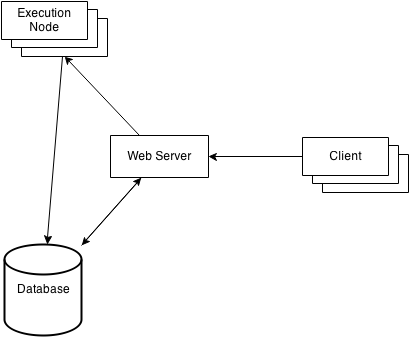
\includegraphics[scale=.5]{chapter06-img1.png} 
 	\caption{System overview}
 	\label{fig:systemOverview}
\end{figure}

\section{Views}

We have chosen to depict the architecture using Philippe
Kruchten's 4+1 view model. [1] This is a method of
describing the architecture for software-intensive systems from the
viewpoint of different stakeholder by using multiple, concurrent views.
We chose this model because it gives a good overview and is widely
accepted by the software industry. Below are the 4 main views in the
model; Logic, Process, Development, and Physical. The
``+1'' view is Use Cases which is
addressed in [Chapter 2 Task Description and Overview]

\subsection{Logic View}
The logical view describes the functionality of the system by breaking
down requirements into classes and representing them, and their
relations, through class and sequence diagrams.
\begin{figure}[h!]
    \centering
	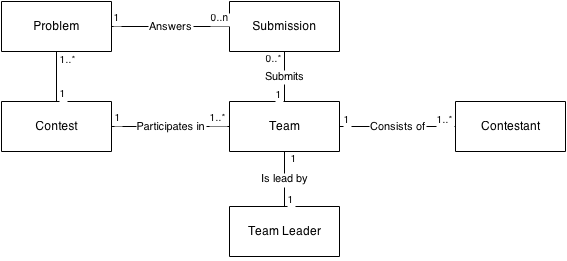
\includegraphics[scale=.5]{chapter06-img2.png} 
	\caption{Top level class diagram}
\end{figure}

Figure 6.1 shows the main classes involved in GentleIDI.\ Each team
participates in a single contest, and consists of a predefined number
of contestants. Each team also has a team leader that handles most of
the administrative tasks. The team can also try to solve problems by
uploading submissions. 

\subsection{Process View}
The process view explains the communication between different processes
in the system, as well as how the system behaves in runtime. 

As this system is a web application the first thing to note is that
there will be concurrent users in runtime. Each user generates HTTP
requests to the server, which in turn may execute database lookups for
information like score tables or problem sets. When a user submits a
solution the system will place it in a queue, which decides which node
the solution will execute on according to availability and load. 

We will now show examples for two important parts of the application.
First is the action of successfully registering a user and creating a
team. See figure~\ref{fig:actRegister}.
\begin{figure}[h!]
    \centering
	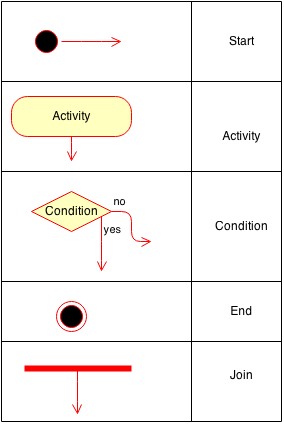
\includegraphics[scale=.5]{chapter06-img3.png} 
	\caption{Symbology}
\end{figure}

\begin{figure}[h]
	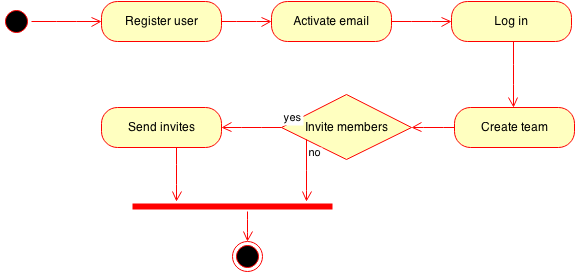
\includegraphics[width=0.8\textwidth]{chapter06-img4.png} 
	\caption{Activity Diagram for registering a user and a team}
	\label{fig:actRegister}
\end{figure}

Second is submitting a solution to a programming problem. See figure~\ref{fig:actSubmit}.
\begin{figure}[h]
	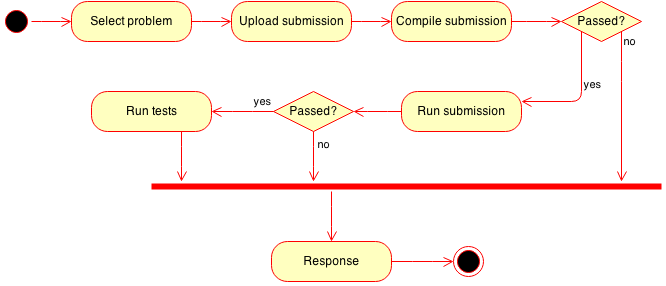
\includegraphics[width=0.8\textwidth]{chapter06-img5.png}
	\caption{Activity Diagram for submittion a solution}
	\label{fig:actSubmit}
\end{figure}

\subsection{Development View}
\subsubsection{Purpose}

The developer view is intended for the developers. It should ease
development, and focus on software module organization by packaging the
software in small chunks.

We wanted a modular and maintainable system where it is easy to maintain
and change specific parts of the system without changing everything.
The structure of the system can therefore be divided into the following
main packages: Contest, Registration, Submission, Execution, Balloon,
Clarification, Admin, and Article. These packages are described in
detail in chapter 8 Implementation. 

\subsection{Physical View}
\label{sec:physicalView}

\subsubsection{Purpose}
The physical view shows the interaction between the physical components
of the system.

Physically the system is structured as a multitiered architecture. It
consists of three tires, presentation tier, application tier, and data
tier, see figure~\ref{fig:multitier}. The tiers represents a physical
structuring mechanism for the system infrastructure. The user is physically
separate from the application and database. 

\begin{figure}[h]
	\centering
	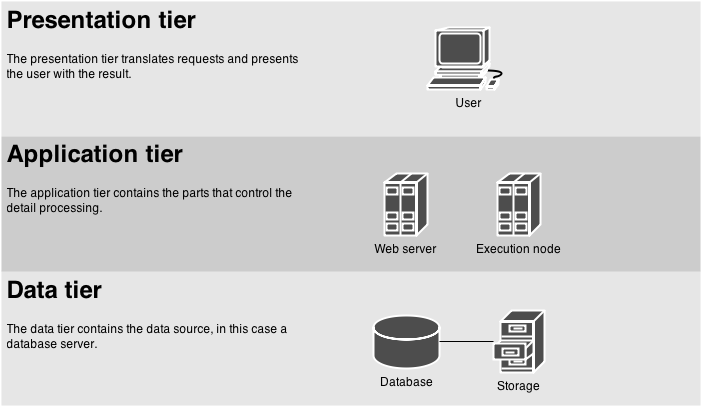
\includegraphics[width=0.8\textwidth]{chapter06-img6.png}
	\caption{Multitier architecture}
	\label{fig:multitier}
\end{figure}
\subsubsection{Presentation tier}

This tier presents information to the user through the public website
and admin interface. It translates the web server response into web
pages generated using HTML5, CSS, Ajax, and JavaScript. It sends
requests to the underlying web server and renders the response.

\subsubsection{Application tier}\label{section:applicationTier}

The application tier contains the logical layer, it controls an
application's functionality by performing detailed
processing. Primarily this is done through python code, although when
running solutions the file is run on an execution node through the use
of built in unix commands. 

This splits the application tier in two parts, the web server that
serves static and dynamic content, and the execution nodes that process
uploaded submissions. This division can be seen in
``Application Tier'' in Figure~\ref{fig:multitier}.


For the web server we use Nginx for serving static files, and as a
reverse proxy for Gunicorn, the server providing dynamic HTTP content
to the user. Gunicorn is the server that processes requests and returns
HTTP pages. The execution nodes process submissions through a FIFO
queue implemented with Celery and RabbitMQ.\ This provides load
balancing across CPU cores and multiple nodes in the cluster. The
execution nodes also share parts of the filesystem, this is implemented
with SSHFS (SSH Filesystem), and is a secure way of sharing the
uploaded files across the execution nodes. 


\subsubsection{Data tier}

This tier includes the data control functionality. The system utilises a
shared SQL database for the execution nodes and the web server. See
Figure~\ref{fig:systemOverview}. This database links to the file storage on the main web
server. However, the execution nodes requires some files to be shared
across multiple nodes. Like explained earlier in
section~\ref{section:applicationTier}, this is implemented with SSHFS.\ For
more specific details see~\ref{chapter:implementation} and~\ref{appendix:ER}.


\section{Quality attributes}

\subsection{Availability}

Since this software is to be used in a programming contest, it is
crucial that the system has high uptime and availability. And since the
contest only lasts for about 4 hours, our margin for failure is
minimal. We have made an effort to account for all possible outcomes,
and to safeguard the application for any errors that might occur. 

\subsection{Modifiability}

This is a system that we hope will be used for many years to come. With
the ever changing nature of the web, the ability to adapt and improve
is imperative. To accommodate this, we chose to implement our solution
in Python, a language taught to most of new students of computer
courses at NTNU.\ These are the same students that hopefully will use
and continue to work on this software. To our best ability we have also
tried to write and document the code in a way such that it is easy to
understand and improve.

\subsection{Performance}

Performance is an important aspect of every application, especially web
applications. Users expect that sites loads fast. Failing to accomplish
this is a sign of a bad application, at least from the
user's perspective. For this reason we have focused on
making our pages load as fast as possible. And since this application
will be used by over 100 users simultaneously, it is also important
that the servers will handle the load. \ 

\subsection{Security}

Since our application contains user data and data that should be hidden
from unauthenticated users, security is another important aspect.
Django provides many security features by default, and others that can
be implemented with very little effort. We also chose to enable SSL on
the web server to increase security on web requests.

\subsection{Testability}

When we first started out, we wanted to utilize testing during
development. Testing is a way to find problems early, and before they
begin to encompass larger parts of the application. But testing is also
one of the most time consuming parts of the development process. In the
end we did not have as much test coverage as we would like, but we feel
that we covered the most important parts.

\subsection{Usability}

As with any web application, we want the users of the system to
accomplish their desired task, and learn the functions of the system
with ease. The user should receive feedback if something went wrong or
if the outcome is not clear. We also want the web pages to provide
information how to use the system. \ 

\section{Patterns}

\subsection{Client-Server}

Since we are making a web application we will use the Client-Server
pattern. The clients connect to the server through a web interface,
either the website or the admin interface. 

\subsection{MVC(model-view-controller)}

The front end is implemented using the Django framework and follows a
rather strict implementation of MVC.\ Every HTTP request sent to the
site is handled by a controller function, which in turn fetches the
appropriate models from a database, creates a view based on the models
and returns the view as an HTTP response. 

\subsection{Shared-Data}

The system utilises multiple execution nodes as well as a web server,
through which users access data. We wanted to have a central shared
database server that scales with the number of execution nodes and the
amount of data. 

\subsection{Multi-tier}

See:~\ref{sec:physicalView} Physical View.
References:

[1] Architectural Views -
% http://www.cs.ubc.ca/\~{}gregor/teaching/papers/4+1view-architecture.pdf


% \chapter{UI Design}
This chapter contains the choices made regarding the process of
designing the front-end of the application, for a more technical
approach see \textit{System Architecture chapter 6}.

\section{Design Process}
\label{sec:designProcess}

The user interface provided by the previous IDI Open system consisted of
a simple web interface for reading news items, registering teams for
contests, and delivering submissions. GentleIDI is intended to provide
more functionality through its web interface, including but not limited
to judge supervision(requirement FJ-11) and user management 
(requirements FC-01, FC-03 and FC-04). As a consequence
we had two options available: reusing and extending the existing
interface design, or creating our own design from scratch.

\begin{figure}[h!]
	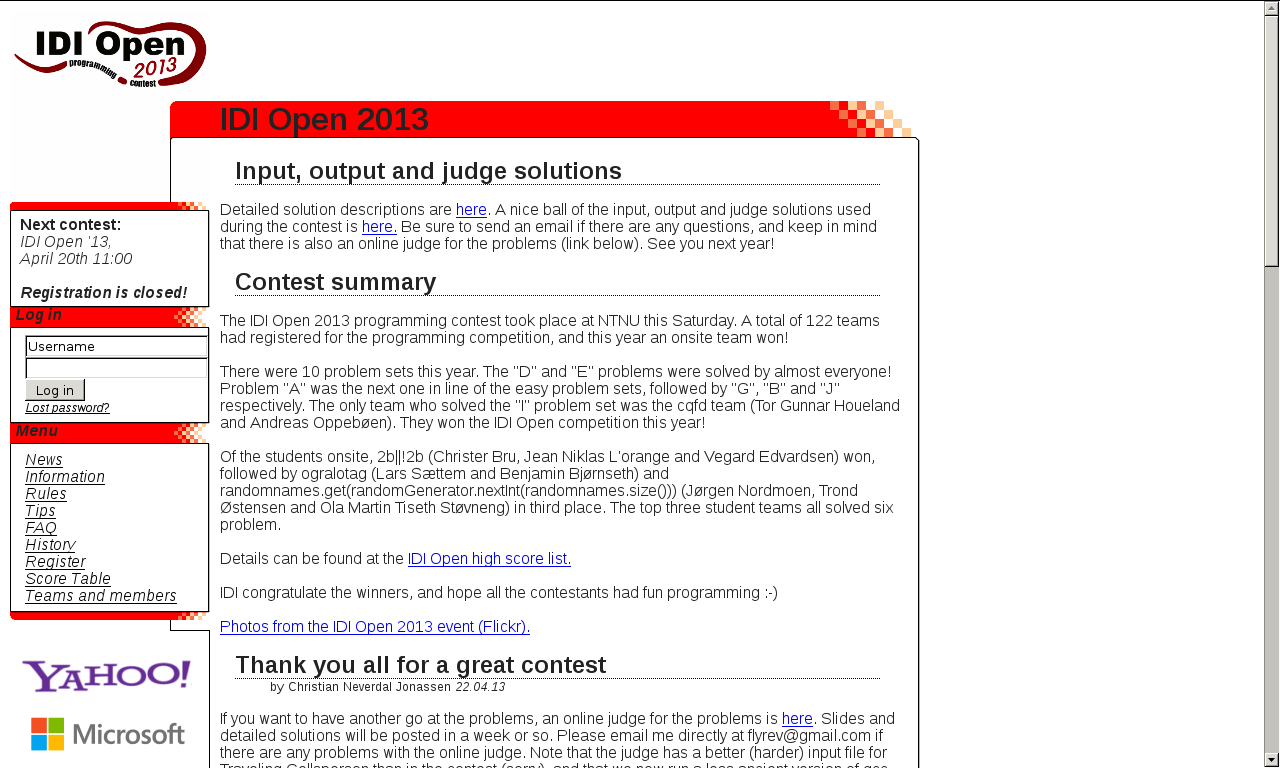
\includegraphics[width=6.278in,height=3.7638in]{a07Design-img1.png} 
	\caption{User Interface of the old system}
	\label{fig:oldSystem}
\end{figure}

We chose to create our own design from scratch, while still trying to
keep a similar placement of elements from the previous design. The
customer expressed concern regarding how contestants would react to the
transition from the old interface to the new one. With this in mind we
started to create mockups modelling core elements of the website. Our
initial drafts consisted of simple rearrangements of elements found in
the old web interface.

\begin{figure}[h!]
	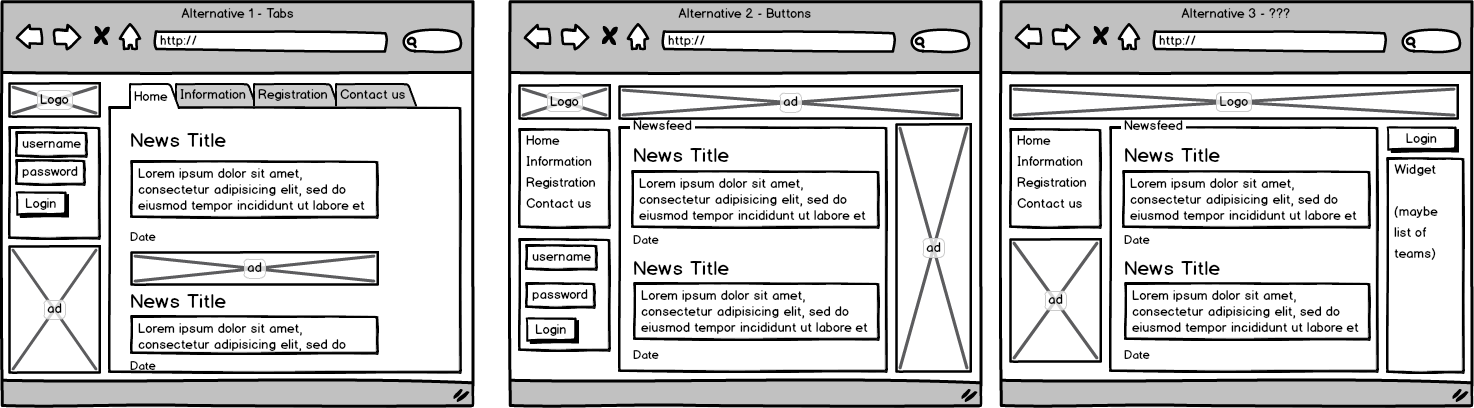
\includegraphics[width=6.278in,height=1.7362in]{a07Design-img2.png} 
	\caption{Initial mockups}
	\label{fig:mockup}
\end{figure}

\pagebreak
Beyond our three initial mockups we tried a couple of ``out
of the box'' approaches to our designs, but none of them
met our standard and was rejected for either being too time-consuming
to implement or too far from what our customer wanted. We had a meeting
with our customer, where we showed our mockups, and what our thoughts
on design had been so far. We wanted to make sure that the customer
was on the same page as us, and that we were not moving beyond the
scope of the project. Our customer was not very focused
on the design aspect, but one demand they had was that they wanted the
new site to have the same structure as the old one. One example of what
this means is that the customer wanted us to keep the menu on the
left side as you can see that the old system has in Fig~\ref{fig:oldSystem}. We agreed,
because getting used to a new website can take time, so keeping the
structure similar would ease the transition for our users. With this in
mind we decided to go for one of our initial mockups, the rightmost one
in Fig~\ref{fig:mockup}, because it had the same structure as the old page, and we
personally favoured that design. As a result, most of the elements
found in the old interface can be found in the new one, and the
transition between using the two is reduced to a minimum.

The task had to be completed in time for milestone M-03, so our main
concern was designing for the functionality needed for that particular
milestone. However, we also had mockups for functionality outside of
this milestone. After milestone M-03 was met, we introduced new designs
for new functionality through continuous work on top of a template.

The majority of the front end is stylized using bootstrap[Link til
kilde] as a framework, enabling us to create a site which is both
highly maintainable and aesthetically pleasing at the same time. The
admin interface was created using django-admin-interface. Grappelli
was used as a skin to give it a modern look. The look of the final page
can be viewed in Fig~\ref{fig:finalUI}.


 \begin{figure}[h!]
	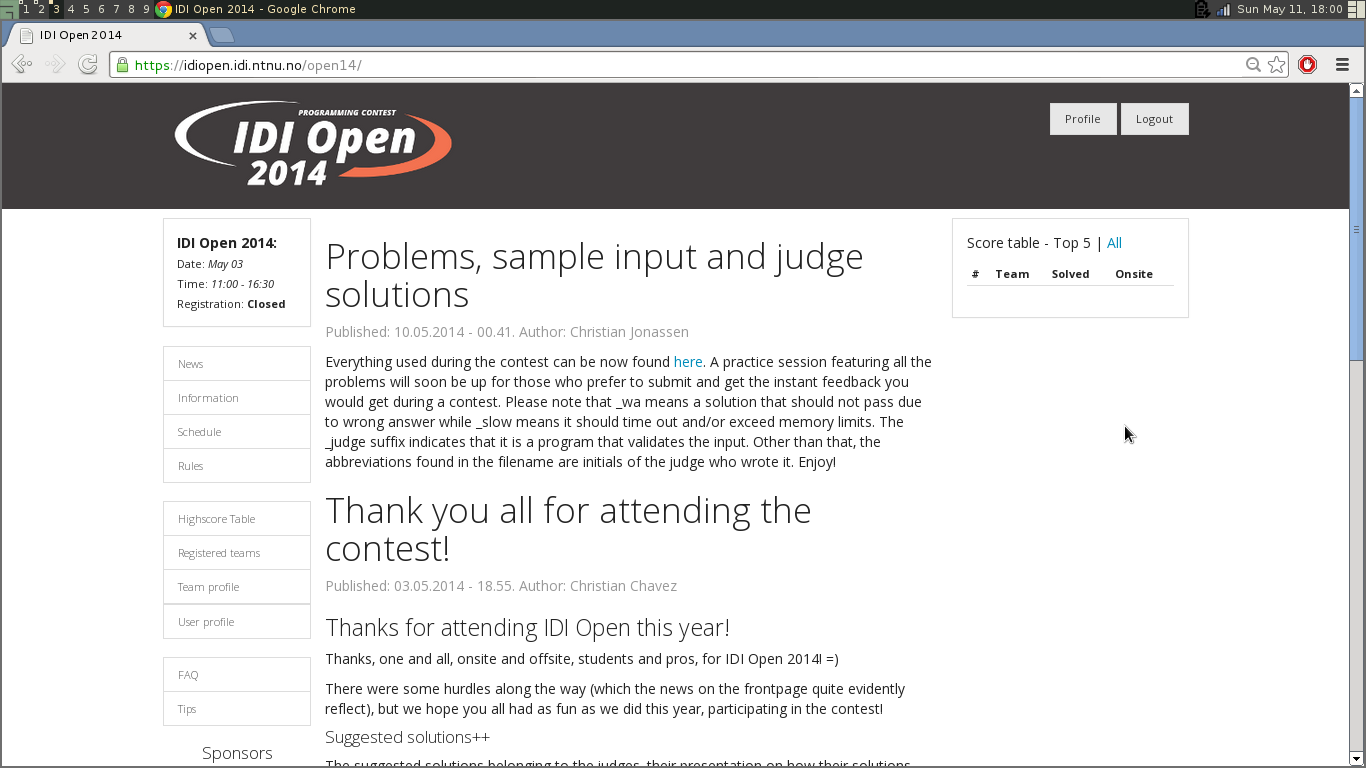
\includegraphics[width=6.4272in,height=3.2602in]{a07Design-img3.png} 
	\caption{Final page}
	\label{fig:finalUI}
\end{figure}

\pagebreak
The grey header was in our
initial design coloured blue, but was changed one week before M-07.
This illustrates the strongest
functionality of the design, namely customization. It is possible, by
only uploading a new CSS file, to change the whole feel of the website
and give every contest its own theme. The change from blue to grey was made
as a consequence of IDI Open changing to a new logo. By comparing
Fig~\ref{fig:oldSystem} and Fig~\ref{fig:finalUI}, you can see that we kept the same structure, but
still made some significant changes to the design.


\section{User Interface}

The user interface is designed by using a base template. The template is
the same for every part of the webpage, and contains a content block
that changes while you navigate through the different parts. This makes
it easier to add new content to the user interface, because you already
have the base, and don't need to worry about the
header, footer, or the menu. We wanted to make it easy for future
developers to take over GentleIDI after us, and therefore we focused on
a versatile user interface, in case they want to add new functionality.

The menu is placed to the left, coping with the western norm stating
that eye placement is natural to the
left\footnote{\url{http://research.microsoft.com/en-us/um/people/cutrell/chi09-buschercutrellmorris-eyetrackingforwebsalience.pdf}}.
We designed the menu to be versatile, this was highly prioritized by our customers.
Admins can choose what they want to show in the menu, except for \textit{Register user} and
\textit{Register team} that are ``hardcoded'' on request from the
customer. As mentioned
in Design process~\ref{sec:designProcess}, we designed the user interface after
a principle of versatility. Admins can also change the logo, the sponsor images
and the contact information in the footer.

Buttons, images and icons were surrounded with boxes, to show that they are
different elements. There is also one big box surrounding a group of elements,
for example the sponsors. This is consistent with the gestalt law of proximity,
that constitutes that humans will naturally group objects that are close to
each other, and view them as distinct. This helps the user quickly understand
the user interface.


\begin{figure}
    \begin{longtable}{|l l l|}
        \hline
        
\includegraphics[width=2.1807in,height=0.5972in]{btn_contestpage.png} &
        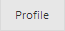
\includegraphics[width=1.0693in,height=0.5in]{btn_profile.png} &
        
\includegraphics[width=1.1528in,height=0.4028in]{btn_leaveteam.png}  \\
        \hline
    \end{longtable}
    \caption{Various buttons used on our website} \label{fig:buttons}
\end{figure}

\pagebreak
``To strive for consistency'' is the
first of Shneiderman's eight golden rules of interface
design\footnote{\url{https://www.cs.umd.edu/users/ben/goldenrules.html}},
and we tried to follow this while making design decisions. As can be
seen in Fig~\ref{fig:buttons}, we decided to use colours that represents the action
each button is connected to. The red button marks that pressing this
will have permanent consequences. We added a textbox prompt that the
user has to answer after pressing a red button, that constitutes to
Schneiderman's fifth and sixth rule, for easy reversal
of actions and error handling. This wasn't added
initially, but we noticed while testing the system that without a
prompt, it could be possible to leave your team by mistake.
 
\begin{figure}[h!]
	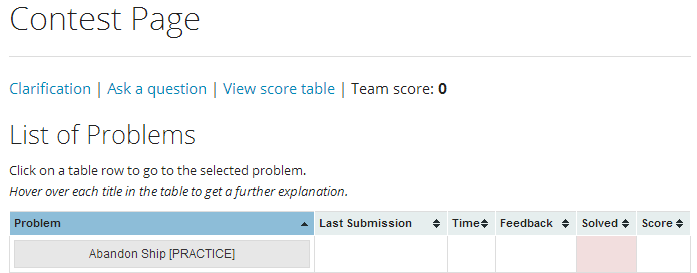
\includegraphics[width=6.5in,height=2.5417in]{contest_page.png} 
	\caption{Contest page}
	\label{fig:contestPage}
\end{figure}

For the contest page, Fig~\ref{fig:contestPage}, we wanted to give the contestant a good
overview of all the problems, their submissions to them, feedback,
if they solved the problem and the score. It is important to not bury
information to deep in a website. It could be challenging to balance
this while trying not to overload the page with too much information.
We had this in mind when designing this page. We got valuable feedback
from the customer concerning what they wanted to be present on the
contest page. They wanted it to be easy for the contestants to access
everything they need during the competition, through the contest page.
After feedback from the customer, we added links to the clarification
page and highscore table on the contest page. This lowers the
short-term memory load on the contestants, which is consistent with
Shneiderman's eight rule, because they will have
everything accessible on the same page.


\pagebreak
\section{Admin Interface}

 \begin{figure}[h!]
     \centering
	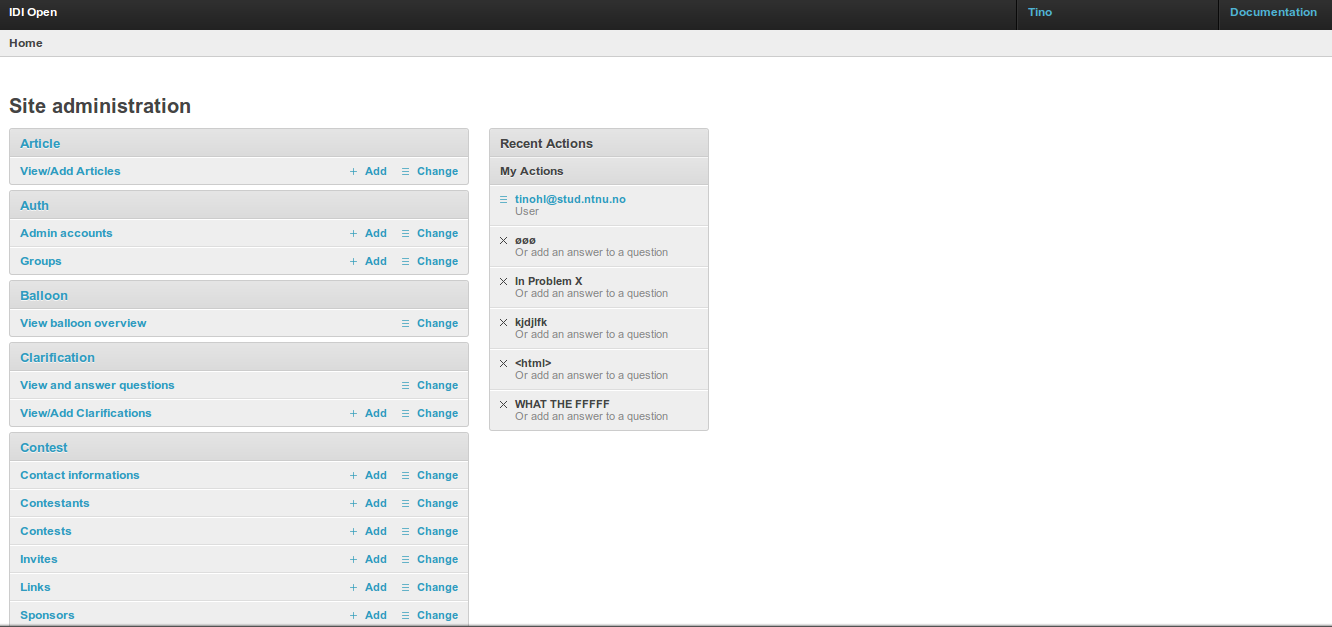
\includegraphics[width=.8\textwidth]{a07Design-img8.png} 
	\caption{Admin Interface}
	\label{fig:adminInterface}
\end{figure}

Django comes with an
extensive admin interface, that provides functionality for adding,
removing and changing parts of the system. The interface consists
of everything we as developers want the admins to be able to change.
We decided to use
Grappelli, an app for the django admin interface that also provided us
with more adequate functionality, e.g.\ auto-completion, rich text
editors, drag'n drop and more.

The structure of the layout is simple. Each category has
it's own header and everything in blue is clickable.
The ``Recent Actions'' box is there
to help admins remember what they last did, which is important to
reduce the users short-term memory load, in accordance with
Shneiderman's eight rule.

Originally all the names of the elements were the same as our model
names. We decided to change this to more intuitively understandable
expressions after a request from the customer.
We extended the interface with our own custom views, ``Balloon overview'' and ``Judge views''. 
This allowed us to change 
what we wanted, while it still kept its consistency with the other parts 
of the admin site.



 \begin{figure}[h!]
	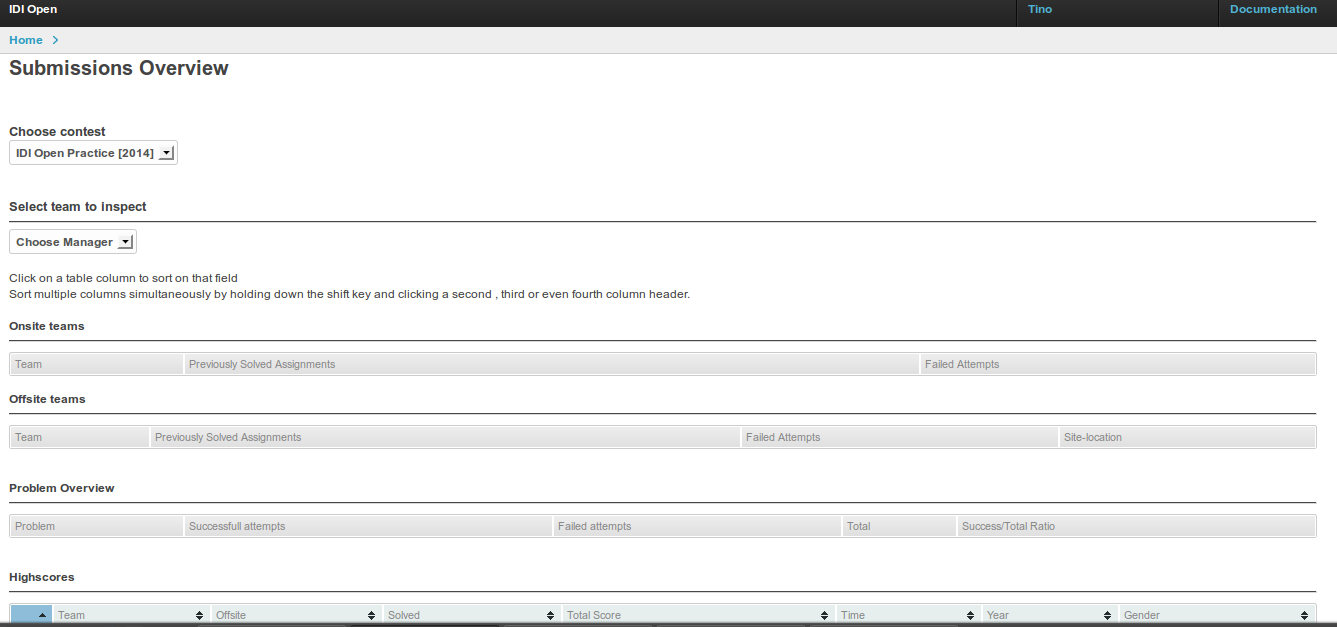
\includegraphics[width=6.5in,height=3.0417in]{a07Design-img9.png} 
	\caption{Judge views}
	\label{fig:judge}
\end{figure}

The judge views was made primarily for judges, but could also be used
by the admins. The motivation behind making this view, is that it gives
the judges a better overview of the competition and how the progress
is going for the different teams. We were initially told that the
judges wanted a way to see if a team was struggling, so they could help
that team. We wanted everything to be on one page for the judges, so they
wouldn't have to constantly switch between different pages. The judge view can be seen in Fig~\ref{fig:judge}.

 \begin{figure}[h!]
	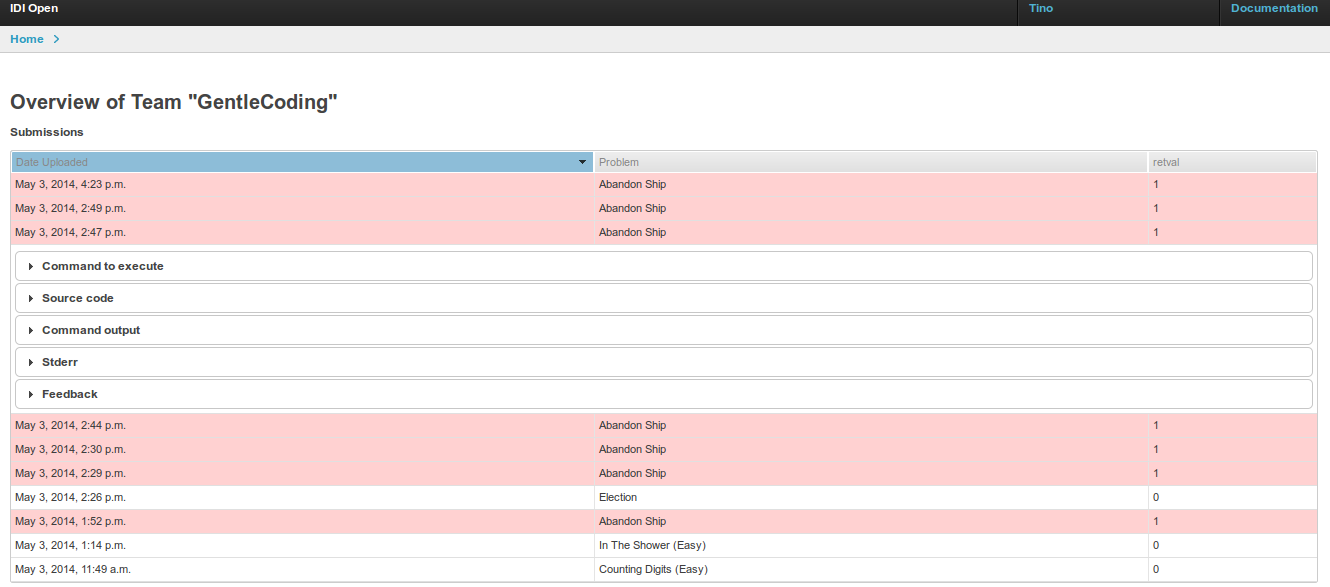
\includegraphics[width=6.5in,height=2.8752in]{a07Design-img10.png} 
	\caption{Judge views for team}
	\label{fig:judgeTeam}
\end{figure}


Fig~\ref{fig:judgeTeam} shows the judge views after selecting the team
``GentleCoding''.
It is possible to expand each submission by clicking on it. The third
submission has been clicked on, so we can now choose to expand
different categories. For example if a judge wants to see the source
code for that submission, he/she can click on ``Source code'' and it will
expand. Submissions that
haven't been compiled are shown in red, and the other are white.

% \chapter{Implementation}

This chapter goes into the details of our implementation. As mentioned
in section X.X, Django follows the MVC pattern in a quite strict
manner, and as a consequence so does our project. In addition to MVC
our project is divided into several Django apps, which are separate
modules containing their own models, views and controllers. The apps
are intended to serve a specific purpose and provide a certain level of
modularity. However, some apps are dependent on others.


\bigskip

\begin{figure}
	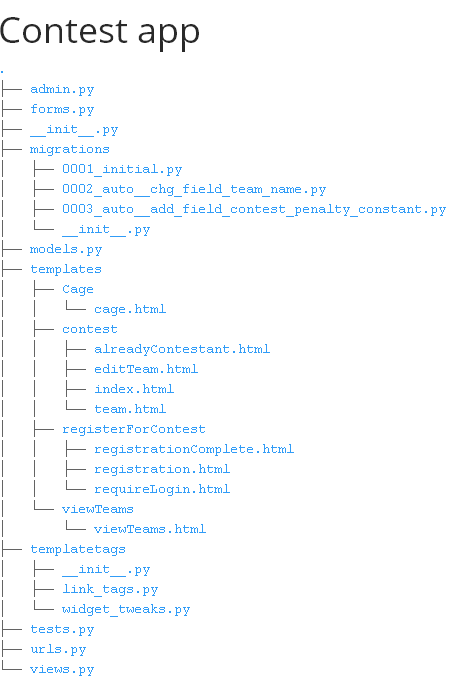
\includegraphics[width=0.8\textwidth]{a07Implementation-img1.png}
	\caption{App overview}
	\label{fig:appOverview}
\end{figure}


\bigskip

Figure~\ref{fig:appOverview} shows the directory structure to one of our apps, all apps
follow this structure. An app{\textquoteright}s root folder contains
four files worth taking a closer look at, models.py, views.py,
forms.py, and admin.py. 


\bigskip

\begin{itemize}
\item models.py contains the app's models i.e. our database entities. Due
to our site being MVC, every aspect of the site is in some way
represented by a model defined in a models.py file.

\item The file views.py defines the app{\textquoteright}s functions for
handling requests, called views. Though the naming might be confusing,
the views defined in this file are not views in the MVC sense of the
word. The views are in essence MVC controllers. When an HTTP request is
received by Django it is routed to a specific view, and the view then
handles the request. Though most views simply serve web pages in
response to GET requests, there are no limits as to what a view can be
used for. 
\item The forms.py file contains a set of Django forms, which are simply
collections of input fields. The forms can be rendered as HTML, and
serve as validators of the input received by POSTs. 

\item This leaves the admin.py file. Django provides a quite modular and
modifiable admin app for managing other apps. The admin
page{\textquoteright}s main functionality is that of viewing, editing,
creating and deleting models. However, the admin app does not have
access to all of the models in the system by default. The admin.py file
is where an app registers which of its models are to be modifiable by
the admin page, how the models are to be rendered etc.

\item The apps also contain a templates directory. The templates are in
essence HTML files extended by Django's template language, making them
easily processed/modified by Django. These templates corresponds to the MVC Views.
When a Django view sends a response it is usually by inserting dynamic
content into a template and then serving the final HTML file as
an HTTP response. Though not visible in the figure, most of our
templates are extensions of a global base template, this way redundancy
is reduced and our user interface stays consistent.
\end{itemize}

\bigskip

\section{contest}
The contest app contains the most fundamental functionality and models for the system,
namely the ones related to creating, hosting, and deleting contests. 
The contest app defines a couple of models
for storing information directly related to a contest, such as sponsor
information, support contact information etc. Just about every
other model in the project is related to the contest models in some way.
A complete overview of the models defined in the contest app can be
found in [reference contest ER]


\bigskip

\section{article}
The article app provides basic functionality for posting news articles.
It contains several different views for looking at articles, lists of
articles etc. For editing articles the app uses a WYSIWYG editor,
available in the admin interface. 

\section{userregistration}
As the name suggests this app handles user creation, deletion and
modification. The majority of this app is an open source app that we
incorporated into our project, however, we made some
modifications of our own. 

\section{teamsubmission}
When a team has reached something they think might be a valid solution
to a problem they submit their source code to the system. The uploaded
source becomes part of a submission model which is part of the
teamsubmission app. This app also defines some models related to the submissions model.

\section{execution}
The system needs a way of handling the submitted source code. For
instance it needs some way of determining which compiler is to be used.
When the source has been built the system needs to know what command is
to be issued to the system to execute the binary. Both of these things
are handled by the execution app. In addition there are restrictions
set to limit the resources available to the submissions, for example
the number of subprocesses, memory allocated etc.


\bigskip

The models defined in teamsubmission and execution can be found in the
[reference submission ER]


\section{node\_manage}
With a well configured system and the previously mentioned apps working
properly, a submitted source file will be stored and the outline of how
the file should be treated will be set when the file is uploaded. The
code for actually performing the actions of building and running is
handled by the node\_manage app. The node\_manage app fetches the
appropriate settings for a submission, and submits it to a FIFO queue.
Our backend consists of several execution nodes connected in a cluster
powered by a framework called Celery. The nodes can be configured to
handle any number of concurrent submissions, and when a node has got
available capacity it fetches another submission from the queue. Celery
relies on the AMQP message passing standard, by means of an open source
message broker system called RabbitMQ. All messages passed go through a
broker setup on the same host as the web server, the broker then
distributes the messages to the appropriate host. 

\section{balloon}
When a team has solved a problem, they are to be awarded a helium
balloon. This app enables staff users to view problems that have newly
been solved by a team, send somebody to deliver a balloon, and then
remove them from the list of newly solved. This app simply provides
a custom view in the Django admin page.

\section{changeemail}
Since we had to modify the userregistration app that we incorporated,
not everything worked as we wanted out of the box. An example was
the functionality for changing the email of a contestant, which broke 
the contestant's pending invites. This app provides a fix for that
problem and makes sure that changing email works properly.

\section{judge\_supervise}
This app provides judges with an interface in which they can see all
submitted solutions and statistics for each team. For each submission,
the judges can see compiler errors, execution output and source code. 

\section{clarification}
During a contest questions can be asked by contestants to the staff. If
a problem is ambiguously formulated, or they are experiencing system
errors, these problems can be addressed by requesting a clarification.
The questions are posted publicly on the website, as well as their replies. \ 


% \chapter{Development}\label{chapter:development}

This document describes the different phases of development the group
went through in order to finish the product. To increase readability
the first part of the document describes the process of working towards the
milestones, as can be viewed in table~\ref{table:milestone}. The second part
describes each sprint in more detail including work done/completed. 

\section{Working Towards the Milestones}
\subsection{Milestone M-01 - Preliminary Report}
\label{sec:M01}

From start to 09.02.2014

Eager to start, we had our first meeting 15.01.2014. During this meeting we
discussed which tasks we wanted apply for After receiving the project
assignment, we discussed our ambitions for the course and the end product. We
agreed that we had a shared goal to receive a top grade in this course, and
that we where all prepared to put in the work required to achieve this goal.
The group was in doubt if we should try popular, enterprise-level tools and
frameworks, or if we should stick to basic, previously used tools. We decided
to let each member of the group to explore a tool on his own and present his
experience to the others. If the tool seemed usable, we incorporated it into
our project.

Our primary concern was that we would spend time on suboptimal tools, methods
or frameworks. Thus, the group spent much time discussing and modeling the
application to come. 

\pagebreak
\subsection{Milestone M-02 - Mid-semester Report}
\label{sec:M02}
From 09.02.2014 to 09.03.2014

Being aware of the large amount of programming ahead of us, we aimed to have
the mid-semester report finished one week before the actual deadline. To
shorten meeting time and strengthen our task overview, we had a meeting
thoroughly discussing how Scrum worked. We decided to adhere more of the
conventional Scrum standard. As a consequence we started to draft release and
product backlogs. This resulted in a reduction in the number of hours used to
administer and delegate tasks. We also got a better overview of what we wanted
the end product to look like. This meant that we could reduce the amount of
modeling, and focus more on the code. 

The mid-semester report finished as planned one week before our deadline. We
more or less completed our testing plans and concluded on management structure.
The biggest challenge was how to implement support for user handling. 

\subsection{Milestone M-03 - First Release}
\label{sec:M03}
From 09.02.2014 to 19.03.2014

Having finished the mid-semester report, the group now had a structured
overview of the requirements specification, and approach to development. We had
much coding to do in order to reach the third milestone. We tried to agree on
an optimal approach, but concluded that we had to ``just get started''. In our
sprint backlogs the amount of coding assignments grew. To induce more coding,
we arranged informal coding nights in order to trigger ``learning by doing''
and improved our progression.

By the time we had finished the necessary prestudies and requirements, we
already had some functionality. However, there was still work remaining, as
suggested by our work breakdown structure. In addition we had a meeting with
the customer where they proposed some new requirements, and reprioritized a few
others. 

In advance to the first release we had some meetings with the customer We
were a little nervous regarding some of the design choices, however, the
meeting discussing the design went well. We had formerly agreed on our mock
up-design, although there were a few discrepancies between the delivery and
what the customer wanted.

The deadline for our first delivery to the customer was 19.03.2014, but the
actual release of the website was delayed to after the weekend, for external
reasons. 

\pagebreak
\subsection{Milestone M-04 - Presentation}
\label{sec:M04}
From 09.02.2014 to 19.03.2014

Since the presentation was scheduled at the same time as our first
release, we did not have time to prepare for this presentation.
Nevertheless, we received valuable feedback from other groups.

\subsection{Milestone M-05 - Beta Release}
\label{sec:M05}
From 19.03 to 11.04

Working toward the beta release was challenging. Increasingly, we
experienced that modeling the application before coding was not an
optimal solution. Thus, we began to code without relying on diagrams to
aid us. We sustained this approach until the end of the project.

With limited time, it became necessary to prioritize some tasks over
others. Our improved product backlog proved to be a
big benefit. As mentioned previously, we felt that it was hard to
predict the outcome of the development process, so we decided not to
update the Gantt diagram. Instead we relied on our own options and
customer prioritizations. This was due to our new understanding of what
needed to be completed when.

We did make some progress with our development, but still had some
aspects of our frameworks that needed to be researched. As the weeks went
by, we increased our work estimates and grew more familiar with the
framework. Still our models seldom related to the actual end result. It
was not something we felt was a big problem, as we where making progress.

\subsection{Milestone M-06 - IDI Open Test Event}
\label{sec:M06}
From 11.04.2014 to 26.04.2014

We still had quite a few packages to implement, and we were uncertain
how much time we needed to spend on each of them. As a consequence
we had to shorten our easter vacation. Spending this much time together,
every day for weeks, may cause tension in groups. We felt it was
important to create an environment to ease the tensions. Therefore we
took breaks from the coding, eating pizza and playing foosball. We started every day discussing what we were suppose to do, similar to a
daily scrum. We believed all members had a good tacit understanding of
what needed to be done, so we transitioned from sprint backlogs to
daily TODO lists. These lists were written informally for the sake of
brevity.\newline
\newline
The days were long, lasting from 09:00 to 24:00. Packages were
implemented at a high pace, and the pieces where finaly starting to fall into place. 
The biggest challenges were to get the execution node up and
running, highscore table, and contest management for the judges. Testing
was also completed. We also had sufficient time to implement some of
the lower prioritized requirements. 

\pagebreak
During the test event, we sat at our own table and received feedback
from the judges and volunteers that had shown up. The fact that some of
the judges were considered really good programmers made us a little
nervous. They did give us feedback and a list of new requirements to be
implemented. These were minor fixes, mostly related to the user
interface. The test event itself was considered a success: all the
judges approved our system.

\subsection{Milestone M-07 - IDI Open}
\label{sec:M07}
From 26.04.2014 to 03.05.2014

After the test event we got a new list of requirements. There was only
one week to the actual event, and we had to carefully pick those we and
the customer felt were the most important. We implemented support for
several execution nodes, refined the contest management, and fixed small
bugs. Some tasks were complex, so it was a challenging to predict if we
would be able to finish them on time. The most advanced task we were
given after the test event, was that the judges wanted a better overview
of the contest. I.e. they wanted access to the whole
competition and all the functionality, before the contest started. The
customer also wanted to be able to export data to CSV and LaTeX. This
task seemed lightweight at first, but turned out to be much more
extensive. While finishing on time, this consumed more hours than
initially planned.

In total there were 92 teams taking part in IDI Open 14, and a total of
214 registered users in the system. When the contest officially started
and the problem set was released, all users simultaneously accessed
the same resource. This caused a spike on the system load. We had been told
by our customer that the old system had previously buckled under the
pressure from this spike. Our system did, however, handle this well. 
Thus, the start of the contest went well. 

At one point the system went down for a few minutes. This was because we
ran out of hard disk space on our main server. In other words, the
system had nowhere to store its data, and was unable to handle the
requests made by users. After a couple of minutes of deleting
unnecessary files, we discovered that for every file that we removed, we
only bought ourselves a couple of more minutes of uptime. Somewhere in
the file system there was a file growing at an alarming pace. 
Identifying this file was challenge. By monitoring the
server's processes we found that the database was logging extensively. 
This resulted in a 1MB/s disk write rate. The rate was small enough that
we could easily monitor and periodically erase the log to clear out
disk space. We could have disabled logging, however, that would have
required a restart of the database server and thereby downtime. 

After this problem was resolved the rest of the contest went without any
significant issues. Our system where capable of handeling a total of 12
concurrent submissions, which was more than enough. All parts of the website where
responsive and working properly, except the highscore list, which we
knew had performance issues. These issues did not have a significant
impact on the user experience.

\pagebreak
\subsection{Milestone M-08 - Final report}
\label{sec:M08}
from 03.05.2014 to 30.05.2014

After the final event we were all exhausted. The following week we only
did some administrative tasks. We started working on the report based on 
the feedback we got from the supervisor and external sources. 

\section{Sprint by sprint}
We have documented each sprint. These are given in appendix
~\ref{chap:sprints}. Below is an example of one of our sprints.

\subsubsection{Sprint 11}
\begin{center}
\tablehead{\hline
\multicolumn{1}{|m{0.5\textwidth}|}{Sprint: 11 } &
Working towards: M-05/M-06\\\hline}
\begin{supertabular}{|m{0.5\textwidth}m{0.5\textwidth}|}
\multicolumn{2}{|m{\textwidth}|}{Overview over packages to be
completed:

\begin{itemize}
	\item Implementation
\end{itemize}
}\\\hline
\multicolumn{2}{|m{\textwidth}|}{Improvements: 

\begin{itemize}
	\item We knew we needed discipline to make it
\end{itemize}
}\\\hline
\multicolumn{2}{|m{\textwidth}|}{Notes:

\begin{itemize}
	\item Parts of this sprint was during easter
	\item This sprint was 11 days
\end{itemize}
}\\\hline
\multicolumn{2}{|m{\textwidth}|}{Packages completed:

\begin{itemize}
	\item Upload submission
	\item Penalty systematized
	\item Review system status
	\item Judge supervisor
	\item Error messages
\end{itemize}
~
}\\\hline
\multicolumn{2}{|m{\textwidth}|}{Summary:

During this sprint, we did not setup a sprint backlog. Instead we kept
an well documented TODO list. Every day all members would tell which
tasks from the TODO list they would work on. At the end of the day we
told each other what was missing. This sprint went great and we were
actually finished some days before M-05-. }\\\hline
\end{supertabular}
\end{center}

\chapter{Testplan}
To determine requirement, structural, and architectural coverage of our
product, software testing has been performed. The tests are formalized
to make it easier to agree on the coverage between the customer,
maintainers, and us. The results and process is documented in this
chapter.

\section{Testing Strategy Overview}
It is common practise to structure tests in three categories. This way,
tests can be communicated to developers, stakeholders, and high-level
non-technical users. 
Following is our interpretation of each category.
\subsection{Unit Testing}
Unit testing is the process of testing program components individually.
The tests invoke methods and structures in the code using different
input parameters. These are usually written before or
immediately after a module is completed. This way, it is easier to
assert that the module does what it is intended. Each test case is
independent from each other, so several people can write test cases
simultaneously without having to worry about dependencies.

\subsection{Integration Testing}
In development, many features are bundled into different components. The
components are then joined together to form a system. The interfaces to 
each of these components, and how they communicate with each other, are tested during Integration
testing. The purpose is to ensure that
communication between the components is correct, and that the
components work as intended. It can be extensive if those responsible
for integration have to review the code in each component, so
integration testing abstract code away. If there are any errors, then
one will either review the unit tests or notify the author.

\subsection{System Testing}
System testing is a high-level test of the system. It is performed after
all of the integrated system parts have been tested and joined
together. System testing is a black box test, as anyone should be able
to perform the test without having any knowledge\ of the underlying
code. The purpose of system testing is to test if our system fulfills
the requirements in the requirement specification. This is important to
find out if we meet the expectations from the customer. 

\subsection{Acceptance Testing}
Acceptance tests are usually executed by the customers. They are written
after agreeing on the requirements specification for a delivery. The
tests are then verified by the customer. Once both the customer and
developers agree on the acceptance test, it will be possible to
formally agree on whether or not a delivery meets the given
requirements.

\subsection{Testing Coverage}
We wanted to provide complete test coverage, unfortunately, due to time contraints we where unable 
to achieve this goal. Thus, we needed to prioritize which components of the system were
most prone to error, and most important to test. The following were our
software assurance objectives:
\begin{itemize}
    \item Ensure that the system can be used by many users
    \item Ensure that the contest can be held without any error that would
critically impact the contest
\end{itemize}

Errors that solely impacted user experience were not prioritized to
test. The majority of these were intended to be found from debugging
the system. Since the developers would work closely with each other, 
we concluded that we would fix small errors in regression.
If our team had more members, or if we had been working in different
locations, this would have been a higher priority.

In most projects, testing is used to ensure requirements coverage. In
our case, however, with frequent customer-meetings and iterative
development, we have not had a strong need for this. The customer has
had access to prototypes of our solution and our source code. In order
to see that the product does as intended, they could simply try it out
for themselves.

As per our software assurance objectives, our largest focus has been
simulating the role of a contestant. To meet our objectives, we
intended to do a full coverage of all contestant scenarios. The
privileged users were believed to be technically experienced and
without intention to do harm. We still felt it was important to prevent
user errors, but our coverage was not as complete for these
usergroups.

Since we were developing a website that would feature many users,
developer testing alone could never simulate peak values for system
demand. We have relied on load testing, giving our Web
server a fixed amount of HTTP requests per second, hereafter RPS.\ What
pages were used in the simulation was determined by us. Thus, our
testing also extends to cover simulated peak values for high loads.

\section{Our Approach to Testing}
This section describes our approach to planning the different testing categories.
\subsection{Unit Testing}

We performed unit testing after the completion of a testable module. The
unit tests use the PyUnit framework, and is written by another person
than the one who produced the code for the module. I.e. if
person A makes module M, then person B will write the unit tests for
module M. The reason for having another person writing the test for a
module is because that will give more people insight in the code, and
make it easier to discover problems. The unit tests reside in the test.py 
file in each Django app.

\subsection{Integration Testing}
Each integration test will test a different interface. The interface is
defined as the connection between the different components in our
system. The pre- and post-condition sets the boundaries for the test.
Input and output is used to determine if the test produces the expected
output with a corresponding input. The motivation behind integration testing is that we
can determine whether a module has been successfully integrated. By
going through the accompanied tests made for the interfaces that
interact with the module


\subsection{System Testing}
Each separate test in the system test is linked to one or more of the
requirements from the requirements specification. This is to ensure 
that the system meets all the requirements set by the customer. The template for
system testing starts with specifying which function is being tested.
After that we say what the action/input should be, and what the
expected result is. The expected result needs to be achieved for the
test to be considered successful.


\subsection{Acceptance Testing}
The customer performed an acceptance test before each release of the
system, so they could confirm that we met the expected requirements.
The acceptance test was based on our system test, with the customer
executing the tasks in the system test. It was
approved when the customer was satisfied with how we implemented the
requirements.

\pagebreak
\section{Testing Results}
The results from our testing is presented in this section.

\subsection{Integration Test}
Each test has a unique identifier, name, pre/post-conditions and corresponding
input and output. An example is given in table~\ref{table:integrationTest}.

\begin{longtable}{|l|l|}
    \caption{Integration test for adding a sponsor} \label{table:integrationTest}\\
\hline
ID & IT-01\\\hline
Interface name & Add sponsor\\\hline
Pre-condtion & Contest is created\\\hline
Post-condition & Sponsor and image\\\hline
Input & Image, URL\\\hline
Output & Sponsor in contest\\\hline
\end{longtable}

In section X.X[12. Evaluation of testing methods] we explained why our
coverage by integration testing was not extensive. The written
integration tests are from our milestone M-03, First release, and only cover the
requirements that was necessary for that milestone. As such, we have
chosen to move all the integration tests to Appendix~\ref{appendix:integrationTest}

We formally agreed on what modules our system was made out of and their
interfaces. Figure~\ref{fig:componentDiagram} shows our view on the system as
per milestone M-03. In figure~\ref{fig:componentDiagram}, we have replaced
some default UML symbols and replaced them with the equivalent UML stereotype.
The explanations are given in table~\ref{table:component}. The integration
tests we did make are given in appendix~\ref{appendix:integrationTest}.

\begin{longtable}{|l|p{.6\textwidth}|}
    \caption{Symbiology for our UML component diagram} \label{table:component} \\
    \hline
    \textbf{UML stereotype} & \textbf{Function}\\
    \hline

    $<<$provides$>>$ & The component delivers the given functionality \\
    \hline

    $<<$requires$>>$& For the component to work it must have the given interface\\
        \hline
\end{longtable}

\begin{figure}[h!]
    \centering
    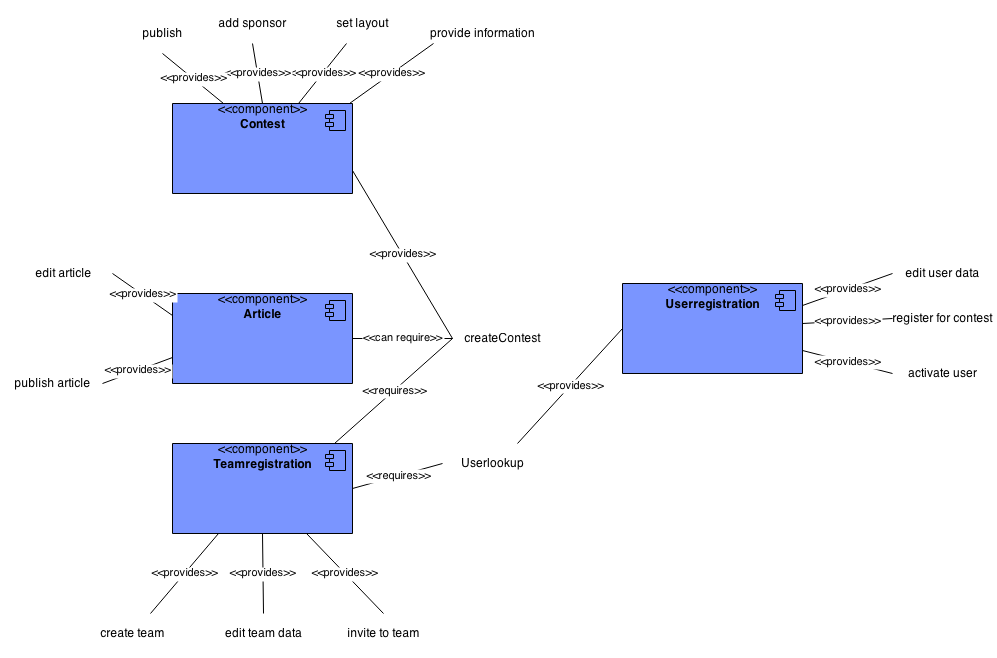
\includegraphics[width=.95\textwidth, height=.85\textheight]{UML_component.png}
    \caption{Diagram from milestone M-03. Each interface connection, especially
    ``createContest'' has been tested}
    \label{fig:componentDiagram}
\end{figure}

\pagebreak
\newpage
\section{System Test}
Our system tests cover all the functional requirements. All tests are
written as successive cases. This means that the tests do not cover
scenarios for how the system should respond when a user performs an
error or another external fault occurs. The complete listing is in
table~\ref{table:systest}.

\begin{longtable}{|l|p{3cm}|p{3cm}|p{3cm}|p{1.1cm}|l|}
\caption[table:systest]{System test} \label{table:systest}\\
\hline
\multicolumn{1}{|c|}{\textbf{ID}} &
\multicolumn{1}{c|}{\textbf{Function}} &
\multicolumn{1}{c|}{\textbf{Action/Input}} &
\multicolumn{1}{c|}{\textbf{Result}} &
\multicolumn{1}{c|}{\textbf{Req}} & 
\multicolumn{1}{c|}{\textbf{Pass/Fail}} \\
\hline 
\endfirsthead

\multicolumn{3}{c}%
{{\bfseries \tablename\ \thetable{} -- continued from previous page}} \\
\hline 
\multicolumn{1}{|c|}{\textbf{ID}} &
\multicolumn{1}{c|}{\textbf{Function}} &
\multicolumn{1}{c|}{\textbf{Action/Input}} &
\multicolumn{1}{c|}{\textbf{Result}} &
\multicolumn{1}{c|}{\textbf{Req}} & 
\multicolumn{1}{c|}{\textbf{Pass/Fail}} \\
\hline 
\endhead

ST-01 & Create a contest, and publish an article to that contest. Edit
article.Then, delete the contest. & Contest name, article text & Contest and
article is no longer publicly    available & FA-16, & PASS\\
\hline

ST-02 & As a contestant, create a team and invite contestants. Go to profile
page and see which team the contestant is amember of. Then, delete the team
& Team, contestants, contest & First contestant in team, then contestant not in
team & FE-01 FE-02 FE-04 FE-06 FC-04& PASS\\
\hline

ST-03 & Add custom css, specify custom settings, & Existing contest, css,
compiler flags, penaltysystem, maximum numbers of contestant, maximum number of
contestant per team & Contest with custom css and settings & FA-05 &
PASS\\
\hline 

ST-04 & Log in as admin, and enable all judges to createa contest. Then remove
and add a judge, by escalating and de-escalating privileges from contestant. &
Admin account, contestant account & Zero changes to system. &
FA-09 & PASS\\
\hline

ST-05 & Log in as judge, create a problem and upload cases. Upload different
solutions; one correct, one erroneous, and one that loops forever. After that,
modify the problem before deleting it.
& Problem, solutions, erroneous code, judge account &
Only the correct solution should give points. &
FJ-01 FJ-02 FJ-03 FJ-04 FJ-05 FJ-06 FJ-07&
PASS\\
\hline

ST-06 & Add two execution nodes with different compiler supports. Change both
nodes, such that they take each other's \ compiler setting. Then remove both
nodes. &
Compiler profiles, available nodes, production server, administrator account &
zero added nodes, no errors in execution & FA-12 FA-13 & PASS\\
\hline 

ST-07 & As a contestant, submit a question to the judge. As a judge, receive a
notification, and answer both the contestant and globally. &
Contestant, contest, question, answer &
All contestants should be able to see message, successful communication between
judge and contestant & FJ-08 & PASS\\
\hline

ST-08 & Create a contestant account. Activate the account via email, and change
the email. Ask for lost password on the new  email. &
Contest-data, emails & Activation data received on the email, and all links
word & FC-01 FC-02 & PASS\\
\hline
\end{longtable}

\pagebreak
\section{Non-functional testing}
% Our non-functional tests ensures non-functional requirements coverage
% and scenario correctness. Additionally, it defines acceptance criteria
% related to the performance of our solution.

The tests related to performance usually comes in pairs, a value and the
double of that value. This applies to the input and expected result.
This is to ensure that system performance does not scale down in a
non-linear way. E.g.\ if ``X''
transactions are processed and the server begins using swap memory
instead of RAM, this would mean that a high load would cause an
exponentially slower load rate for a high number of transactions.

Often, as mentioned in section X.X, we did
inspection tests. Thus, table~\ref{table:not} does not contain all tests that
are executed, and the table only covers the first 12 non-functional
requirements. The documented tests do, however, ensure some
requirements coverage.

\begin{longtable}{|p{4.3cm}|p{2.0cm}|l|p{3.8cm}|l|}
    \caption{System tests} \label{table:not} \\
\hline \multicolumn{1}{|c|}{\textbf{Case}} &
\multicolumn{1}{c|}{\textbf{Input}} &
\multicolumn{1}{c|}{\textbf{ID}} &
\multicolumn{1}{c|}{\textbf{Expected Result}} &
\multicolumn{1}{c|}{\textbf{Pass/Fail}} \\
\hline 
\endfirsthead

\multicolumn{3}{c}%
{{\bfseries \tablename\ \thetable{} -- continued from previous page}} \\
\hline \multicolumn{1}{|c|}{\textbf{Case}} &
\multicolumn{1}{c|}{\textbf{Input}} &
\multicolumn{1}{c|}{\textbf{ID}} &
\multicolumn{1}{c|}{\textbf{Expected Result}} &
\multicolumn{1}{c|}{\textbf{Pass/Fail}} \\
\hline 
\endhead

Adding 500 contestants & 500 users & NF-04 & Ability to add yet another & PASS\\
\hline
Adding 200 teams & 200 teams & NF-05 & Ability to add yet another & PASS\\
\hline
Adding 20 judges & 20 judges & NF-06 & Ability to add yet another &
PASS\\
\hline
Adding more than one admin &
$>$ 1 admin & NF-07 & Ability to add yet another & PASS\\
\hline
Upload a solution which is less than 50kB & Solution $>$ 50kB & NF-08 & Successful delivery & PASS\\
\hline
Upload a solution which is greater than 50kB & Solution $>$ 50kB & NF-08 & Error message & PASS\\
\hline
Gather some test persons not familiar with the system and have them use the
system as a contestant & System & NF-09 & They should be familiar with the
system after 5 minutes & FAIL\\
\hline
Gather some test persons not familiar with the system and have them use the
system as a judge & System & NF-11 & They should be familiar with the system
after 10 minutes & PASS\\
\hline
Gather some test persons not familiar with the system and have them use the
system as an admin & System & NF-10 & They should be familiar with the system
after 15 minutes & PASS\\
\hline
Page responsiveness with at least 5 RPS & HTTP GET and POST to all pages &
NF-01 & Response-time {\textless} 150 ms & FAIL\\
\hline
Page responsiveness with at least 10 RPS & HTTP GET and POST to all pages &
NF-01 & Response-time {\textless} 300 ms & FAIL\\
\hline
\end{longtable}


% \chapter{Risk Management Framework}
A risk is an event or condition that, if it occurs, could have a
negative effect on a project's objectives. To avoid these risks, and to be
able to deal with them effectively, we established a risk modelling framework.
Our framework is based upon our own experience and examples from the many
documents that exists on the subject.

By explicitly writing down corresponding actions for risks that occur,
we could deal with risks without disagreements. It also let external
parties get an overview of what risks we are aware of, and how we
reviewed them. The external party can then notify us of unknown risks
or modifications to our priorities. 
Terminology and Categories

To structurize our risk register, we divided each into the following
categories:
\begin{itemize}
    \item \textbf{Budget risks} are all risks that can be associated with
        financial aspects of our project.
    \item \textbf{Organizational risks} are those that might arise because of
    group structure and task delegation.
    \item \textbf{People Management} comprises all risks associated with team
        management and each individual in the group.
    \item \textbf{Requirements risks} are related to errors in requirements
        engineering.
    \item \textbf{Schedule risks} are about meeting deadlines and task
        delegation.
    \item \textbf{Technology and tools}; product talk about technical risks that
        might arise with tools and our product.
\end{itemize}

To prioritize our risks, we have also given each risk a probability,
consequence and total risk, abbreviated Pr, C, TR, respectively. Each
of these were assigned values from 1-10, where 10 indicated
``very high''. A 10 translates to
the following for each field:
\begin{itemize}
    \item \textbf{Consequence}: event of risk will be fatal to our project.
    \item \textbf{Probability}: risk will probably happen
    \item \textbf{Total risk}: The risk is a big threat and should be monitored closely.
\end{itemize}

Total risk is calculated as Consequence x Probability. By multiplying
these numbers, we get a sorted list of the most dangerous risks. 
Scope of Risk Assessment
Finding the right balance to the extent of documentation is difficult.
Extensive risk-frameworks can consume more hours in maintenance than
they save. To deal with our lacking experience, we only wanted to
document the most likely risks. To us, this meant only including risks
with a total risk value of more than 30

We considered specifying additional information to each risk, like
context and associated risks. However, we felt every member of the
group had a similar understanding of the risks, so writing this
information down would be superfluous. In addition, since the risks
were orally reviewed, we did not want to rely too much on what had been
written down.

\section{Risk Identification}
We tried to involve every group member in the making of the risk
register. The estimates from 1 to 10 were assigned based on our own
experience from previous projects. The list was filled out by three
members of the group, and then later presented to the whole group for
reviewal and agreement on the values. 

Risks that became known in later parts of our development was promptly
added to our risk register. We expected few of these, and few did
occur, so we have not performed any revision control. Our means of identifying
risks was through discussions and agreements that we were not
performing optimally.

\section{Risk Monitoring}
Our primary method for surveilling risks was weekly discussions. In
these meetings, we had open discussions of the group's
progress and development. In addition, we had one monthly meeting where
we would discuss the risks more thorough and in-depth. This involved
re-discussion of the group's expectations and our
involvement in the project. These monthly meetings were referred to as
``snapshots''. The snapshots
specifically addressed the problem that many projects start out quite
ambitiously, but tend to deteriorate, something we wanted to avoid.

To avoid groupthink\footnote{The concept of trying to avoid conflict
by not speaking one's mind. For more, see:
http://www.psysr.org/about/pubs\_resources/groupthink\%20overview.htm}
and complacency, we required each group member on our weekly meetings
to mention three good and three negative points. After that, each
member could bring up extra topics for discussion. For each discussion,
we made sure to be conclusive by explicitly writing how to deal with a
given problem. 

We have frequently involved the supervisor and customer in our process.
We made sure to ask for insights on our development progress. After
each meeting we also wrote down meeting minutes and a summary. This was
later sent to the respective party to ensure agreement on what had been
concluded in the meeting.

\section{Complete List of Risks}
We have chosen to put the complete list in appendix~\ref{appendix:risk_list}.

% \appendix
% \chapter{Sprints}
\label{chap:sprints}

This appendix holds an overview over our sprints, throughout the
project. For a more complete list over packages completed see Appenix~\ref{appendix:burndown}.
This is just an overview were we are trying to bring out the more
important aspects of our sprints. 

\section{Template}
\begin{center}
\tablehead{\hline
\multicolumn{1}{|m{0.5\textwidth}|}{Sprint: {\textless}sprint
nr{\textgreater} } &
Working towards: {\textless}insert milestone\\\hline}
\begin{supertabular}{|m{0.5\textwidth}m{0.5\textwidth}|}
\multicolumn{2}{|m{\textwidth}|}{Overview over packages to be
completed:

{\textless}Insert packages to be completes{\textgreater}

~
}\\\hline
\multicolumn{2}{|m{\textwidth}|}{Improvements: 

{\textless}insert list over things we want to improve about
ourself{\textgreater}

~
}\\\hline
\multicolumn{2}{|m{\textwidth}|}{Notes:

}\\\hline
\multicolumn{2}{|m{\textwidth}|}{Packages completed:

{\textless}insert packages actually completed{\textgreater}

~
}\\\hline
\multicolumn{2}{|m{\textwidth}|}{Summary:

{\textless}A brief summary over the most important
aspects{\textgreater}}\\\hline
\end{supertabular}
\end{center}
\clearpage

\section{Sprint 0a}
\begin{center}
\tablehead{\hline
\multicolumn{1}{|m{0.5\textwidth}|}{Sprint: 0a} &
Working towards: M-01\\\hline}
\begin{supertabular}{|m{0.5\textwidth}m{0.5\textwidth}|}
\multicolumn{2}{|m{\textwidth}|}{
Overview over packages/tasks to be completed:

\begin{itemize}
	\item Get an overview over the course
	\item Get to know the old system
\end{itemize}
~
}\\\hline
\multicolumn{2}{|m{\textwidth}|}{Improvements: 

~

~
}\\\hline
\multicolumn{2}{|m{\textwidth}|}{Notes:

\begin{itemize}
	\item This was the first meeting after getting the assignment
\end{itemize}
}\\\hline
\multicolumn{2}{|m{\textwidth}|}{Packages completed:
}\\\hline
\multicolumn{2}{|m{\textwidth}|}{Summary:

This was still early in the process so most of the time was spent
getting an overview over the whole thing. }\\\hline
\end{supertabular}
\end{center}
\clearpage

\section{Sprint 0b}
\begin{center}
\tablehead{\hline
\multicolumn{1}{|m{0.5\textwidth}|}{Sprint: 0-b } &
Working towards: M-01\\\hline}
\begin{supertabular}{|m{0.5\textwidth}m{0.5\textwidth}|}
\multicolumn{2}{|m{\textwidth}|}{Overview over packages to be
completed:

\begin{itemize}
	\item Read and learn the requirement received from the customer
	\item Set up tools we need in development and process management
	\item Establish Project management framework
	\item Learning tools and framework
\end{itemize}
~
}\\\hline
\multicolumn{2}{|m{\textwidth}|}{Improvements: 

\begin{itemize}
	\item A better meeting structure
\end{itemize}
~
}\\\hline
\multicolumn{2}{|m{\textwidth}|}{Notes:

~
}\\\hline
\multicolumn{2}{|m{\textwidth}|}{Packages completed:

\begin{itemize}
	\item Tools for communication was set up 
    \item Initial requirement elicitation
    \item Initial learning tools prestudy phase
\end{itemize}
}\\\hline
\multicolumn{2}{|m{\textwidth}|}{Summary:

Learning to know the requirements and the subject as a whole was our
main concern at this stage. We also did some research on what framework
we should use. }\\\hline
\end{supertabular}
\end{center}

\clearpage
\section{Sprint 1}
\begin{center}
\tablehead{\hline
\multicolumn{1}{|m{0.5\textwidth}|}{Sprint: 1} &
Working towards: M-01\\\hline}
\begin{supertabular}{|m{0.5\textwidth}m{0.5\textwidth}|}
\multicolumn{2}{|m{\textwidth}|}{Overview over packages to be
completed:

\begin{itemize}
	\item Project management
	\item Install and learn tools we need in development
	\item Begin documenting our process
\end{itemize}
~
}\\\hline
\multicolumn{2}{|m{\textwidth}|}{Improvements: 

~

~
}\\\hline
\multicolumn{2}{|m{\textwidth}|}{Notes:

\begin{itemize}
	\item Tino and Eirik was sent out on seminar. Learning about SCRUM
	\item Trying to use ICEScrum for Scrum related activites
\end{itemize}
}\\\hline
\multicolumn{2}{|m{\textwidth}|}{Packages completed:

\begin{itemize}
	\item WBS
    \item Agreed on using Django as a framework
	\item Risk assignment
	\item Functional requirements
	\item Class diagram 
\end{itemize}
}\\\hline
\multicolumn{2}{|m{\textwidth}|}{Summary:

Most of the tools was set up, we started to some modelling, in order to
get a better overview over the system to be implemented. This was also
documentations to be used in the report. We also systematized the
requirements in order to communicate with the customer. Project roles
was also distributed.}\\\hline
\end{supertabular}
\end{center}
\clearpage

\section{Sprint 2}
\begin{center}
\tablehead{\hline
\multicolumn{1}{|m{0.5\textwidth}|}{Sprint: 2} &
Working towards: M-01\\\hline}
\begin{supertabular}{|m{0.5\textwidth}m{0.5\textwidth}|}
\multicolumn{2}{|m{\textwidth}|}{Overview over packages to be
completed:

\begin{itemize}
	\item Project management
\end{itemize}
~
}\\\hline
\multicolumn{2}{|m{\textwidth}|}{Improvements: 

~
}\\\hline
\multicolumn{2}{|m{\textwidth}|}{Notes:

~
}\\\hline
\multicolumn{2}{|m{\textwidth}|}{Packages completed:

\begin{itemize}
	\item Requirement specification
	\item System architecture
	\begin{itemize}
		\item Flow charts
		\item class diagrams
	\end{itemize}
	\item ER-Models
	\item Preliminary report
\end{itemize}
~
}\\\hline
\multicolumn{2}{|m{\textwidth}|}{Summary:

At this point we had a rough understanding of the work ahead of us, and
we were able to start modelling possible solutions. This was also close
to the deadline for the preliminary report and as a consequence a lot
of time was spent on the report. }\\\hline
\end{supertabular}
\end{center}
\clearpage

\section{Sprint 3}
\begin{center}
\tablehead{\hline
\multicolumn{1}{|m{0.5\textwidth}|}{Sprint: 3} &
Working towards: M-02\\\hline}
\begin{supertabular}{|m{0.5\textwidth}m{0.5\textwidth}|}
\multicolumn{2}{|m{\textwidth}|}{Overview over packages to be
completed:

\begin{itemize}
	\item Inital development
    \item UML Sequence Diagrams, component diagrams,
    \item Initial tests
\end{itemize}
}\\\hline
\multicolumn{2}{|m{\textwidth}|}{Improvements: 

\begin{itemize}
	\item Better sprint planning
	\item We should improve our task delegation
	\item We should prioritize tasks
\end{itemize}
~
}\\\hline
\multicolumn{2}{|m{\textwidth}|}{Notes:

~
}\\\hline
\multicolumn{2}{|m{\textwidth}|}{Packages completed:

\begin{itemize}
    \item UML Diagrams
\end{itemize}
~
}\\\hline
\multicolumn{2}{|m{\textwidth}|}{Summary:

During the past two sprints we had primarily been planning and doing
administrative tasks. This sprint marked the end of that phase. We moved on to
actual implementing. However, we ere not familiar with the tools and frameworks
available to us, and as a consequence we decided to use this sprint to get
everyone up to date on Django/Python. We had a coding night this sprint.
Working all members together. }\\\hline
\end{supertabular}
\end{center}
\clearpage

\section{Sprint 4}
\begin{center}
\tablehead{\hline
\multicolumn{1}{|m{0.5\textwidth}|}{Sprint: 4 } &
Working towards: M-02\\\hline}
\begin{supertabular}{|m{0.5\textwidth}m{0.5\textwidth}|}
\multicolumn{2}{|m{\textwidth}|}{Overview over packages to be
completed:

\begin{itemize}
	\item User-interface design
    \item Project management (schedules, plans)
\end{itemize}
~

~
}\\\hline
\multicolumn{2}{|m{\textwidth}|}{Improvements: 

\begin{itemize}
	\item The activity diagrams does not reflect upon our actual work done.
\end{itemize}
~

~
}\\\hline
\multicolumn{2}{|m{\textwidth}|}{Notes:

~
}\\\hline
\multicolumn{2}{|m{\textwidth}|}{Packages completed:

\begin{itemize}
	\item Agreed on the design for the user interface
\end{itemize}
~
}\\\hline
\multicolumn{2}{|m{\textwidth}|}{Summary:

During sprint 4 we knew we had to improve our WBS. We had a long meeting
where we rebuild our backlog, reviewed SCRUM and created a release- and
backlog. We agreed on user interface design and begun early protoypes}\\\hline
\end{supertabular}
\end{center}
\clearpage

\section{Sprint 5}
\begin{center}
\tablehead{\hline
\multicolumn{1}{|m{0.5\textwidth}|}{Sprint: 5} &
Working towards: M-02\\\hline}
\begin{supertabular}{|m{0.5\textwidth}m{0.5\textwidth}|}
\multicolumn{2}{|m{\textwidth}|}{Overview over packages to be
completed:

\begin{itemize}
    \item Development
	\item Report 
	\item Testplan
\end{itemize}
~
}\\\hline
\multicolumn{2}{|m{\textwidth}|}{Improvements: 
}\\\hline
\multicolumn{2}{|m{\textwidth}|}{Notes:

\begin{itemize}
	\item This sprint we had a meeting with the supervisor discussing the
		  activity diagrams. She suggested that we switch them with our
          own sprint backlogs.
\end{itemize}
}\\\hline
\multicolumn{2}{|m{\textwidth}|}{Packages completed:

\begin{itemize}
    \item Testplan (for current system)
    \item Reviewing our report
\end{itemize}
~

~
}\\\hline
\multicolumn{2}{|m{\textwidth}|}{Summary:

We had a good overview over what should be in the report at this point.
A finished version was right around the corner. In general, this weeks
meeting went much faster than the last. The group was happy about that.
}\\\hline
\end{supertabular}
\end{center}
\clearpage

\section{Sprint 6}
\begin{center}
\tablehead{\hline
\multicolumn{1}{|m{0.5\textwidth}|}{Sprint: \ 6} &
Working towards: M-02/M-03\\\hline}
\begin{supertabular}{|m{0.5\textwidth}m{0.5\textwidth}|}
\multicolumn{2}{|m{\textwidth}|}{Overview over packages to be
completed:

\begin{itemize}
	\item Finish our mid-term report
\end{itemize}
~
}\\\hline
\multicolumn{2}{|m{\textwidth}|}{Improvements: 
~
}\\\hline
\multicolumn{2}{|m{\textwidth}|}{Notes:
Most of the time spent was concentrated on the report.

~
}\\\hline
\multicolumn{2}{|m{\textwidth}|}{Packages completed:

\begin{itemize}
	\item Mid-term report
	\item User-interface completed in bootstrap
\end{itemize}
~
}\\\hline
\multicolumn{2}{|m{\textwidth}|}{Summary:

This sprint we finished the mid-term report and the user-interface was
completed. We were happy with the result. We also finished the mid-term
in good time before the actual delivery. }\\\hline
\end{supertabular}
\end{center}
\clearpage

\section{Sprint 7}
\begin{center}
\tablehead{\hline
\multicolumn{1}{|m{0.5\textwidth}|}{Sprint: 7} &
Working towards: M-03/M-04\\\hline}
\begin{supertabular}{|m{0.5\textwidth}m{0.5\textwidth}|}
\multicolumn{2}{|m{\textwidth}|}{Overview over packages to be
completed:

\begin{itemize}
	\item Presentation
	\item Implementation
	\item Write unit tests. 
\end{itemize}
~
}\\\hline
\multicolumn{2}{|m{\textwidth}|}{Improvements: 

\begin{itemize}
	\item We need to improve our efficieny in pair programming.
\end{itemize}
~

~
}\\\hline
\multicolumn{2}{|m{\textwidth}|}{Notes:

~
}\\\hline
\multicolumn{2}{|m{\textwidth}|}{Packages completed:

\begin{itemize}
	\item Login completed
	\item User registration completed
	\item Team
registration completed\end{itemize}
~
}\\\hline
\multicolumn{2}{|m{\textwidth}|}{Summary:

During this sprint we had boost with the implementation. We were busy
making our first release. Unfortunately we did not have time to set up
the solution live this sprint. It was postponed to after the weekend.
}\\\hline
\end{supertabular}
\end{center}
\clearpage

\section{Sprint 8}
\begin{center}
\tablehead{\hline
\multicolumn{1}{|m{0.5\textwidth}|}{Sprint: 8} &
Working towards: M-05\\\hline}
\begin{supertabular}{|m{0.5\textwidth}m{0.5\textwidth}|}
\multicolumn{2}{|m{\textwidth}|}{Overview over packages to be
completed:

\begin{itemize}
	\item Testing
	\item Set up solution live
	\item Fixing bugs
	\item Peer evalutaion
\end{itemize}
~
}\\\hline
\multicolumn{2}{|m{\textwidth}|}{Improvements: 
    We should increase our test coverage
}\\\hline
\multicolumn{2}{|m{\textwidth}|}{Notes:

}\\\hline
\multicolumn{2}{|m{\textwidth}|}{Packages completed:

\begin{itemize}
	\item Testing
	\item Bug fixing
	\begin{itemize}
		\item Change email
		\item Forgot password
	\end{itemize}
\item Peer evalutaion
\end{itemize}
~
}\\\hline
\multicolumn{2}{|m{\textwidth}|}{Summary:

After we put the solution up, there was some bugs and testing to be done.
We had not had the opportunity to test, by our standards, yet. We did
this while the solution was live. }\\\hline
\end{supertabular}
\end{center}
\clearpage

\section{Sprint 9}
\begin{center}
\tablehead{\hline
\multicolumn{1}{|m{0.5\textwidth}|}{Sprint: 9} &
Working towards: M-05\\\hline}
\begin{supertabular}{|m{0.5\textwidth}m{0.5\textwidth}|}
\multicolumn{2}{|m{\textwidth}|}{Overview over packages to be
completed:

\begin{itemize}
	\item Implementation
	\item Permission testing
	\item user manual
	\item Project mamagement
\end{itemize}
~
}\\\hline
\multicolumn{2}{|m{\textwidth}|}{Improvements: 

\begin{itemize}
	\item We had to be more consistent with testing
	\item Better to fill out sprint documents. 
\end{itemize}
~
}\\\hline
\multicolumn{2}{|m{\textwidth}|}{Notes:

\begin{itemize}
	\item We received the Peer Evaluation. 
\end{itemize}
}\\\hline
\multicolumn{2}{|m{\textwidth}|}{Packages completed:

\begin{itemize}
	\item Possible to upload solutions
	\item Models 
\end{itemize}
~
}\\\hline
\multicolumn{2}{|m{\textwidth}|}{Summary:

This sprint was probably our worst planned sprint. With better planning
we could have finished a lot more coding. Unfortunately this was not
the case and we spent unnecessary much time in the wrong direction. We
were, however happy with our peer evaluation. }\\\hline
\end{supertabular}
\end{center}
\clearpage

\section{Sprint 10}
\begin{center}
\tablehead{\hline
\multicolumn{1}{|m{0.5\textwidth}|}{Sprint: 10} &
Working towards: M-05\\\hline}
\begin{supertabular}{|m{0.5\textwidth}m{0.5\textwidth}|}
\multicolumn{2}{|m{\textwidth}|}{Overview over packages to be
completed:

\begin{itemize}
	\item Implementation
\end{itemize}
~
}\\\hline
\multicolumn{2}{|m{\textwidth}|}{Improvements: 

\begin{itemize}
	\item Still improvement to been done with filling out sprint backlog.
\end{itemize}
~
}\\\hline
\multicolumn{2}{|m{\textwidth}|}{Notes:

\begin{itemize}
	\item This sprint was 9 days long
\end{itemize}
}\\\hline
\multicolumn{2}{|m{\textwidth}|}{Packages completed:

\begin{itemize}
	\item Implementation
	\begin{itemize}
		\item Execution nodes
		\item Compiler profiles
		\item Upload solution
	\end{itemize}
\end{itemize}
}\\\hline
\multicolumn{2}{|m{\textwidth}|}{Summary:

This was the last sprint before Easter. We were more thrilled with this
sprint but. we knew had to shorten our easter vacation. We had a good
start with much of the implementation and we finally felt like we had a
good overview over everything.}\\\hline
\end{supertabular}
\end{center}
\clearpage

\section{Sprint 11}
\begin{center}
\tablehead{\hline
\multicolumn{1}{|m{0.5\textwidth}|}{Sprint: 11 } &
Working towards: M-05/M-06\\\hline}
\begin{supertabular}{|m{0.5\textwidth}m{0.5\textwidth}|}
\multicolumn{2}{|m{\textwidth}|}{Overview over packages to be
completed:

\begin{itemize}
	\item Implementation
\end{itemize}
}\\\hline
\multicolumn{2}{|m{\textwidth}|}{Improvements: 

\begin{itemize}
	\item We knew we needed discipline to make it
\end{itemize}
}\\\hline
\multicolumn{2}{|m{\textwidth}|}{Notes:

\begin{itemize}
	\item Parts of this sprint was during easter
	\item This sprint was 11 days
\end{itemize}
}\\\hline
\multicolumn{2}{|m{\textwidth}|}{Packages completed:

\begin{itemize}
	\item Upload submission
	\item Penalty systematized
	\item Review system status
	\item Judge supervisor
	\item Error messages
\end{itemize}
~
}\\\hline
\multicolumn{2}{|m{\textwidth}|}{Summary:

During this sprint, we did not setup a sprint backlog. Instead we kept
an well documented TODO list. Every day all members would tell which
tasks from the TODO list they would work on. At the end of the day we
told each other what was missing. This sprint went great and we were
actually finished some days before M-05-. }\\\hline
\end{supertabular}
\end{center}
\clearpage

\section{Sprint 12}
\begin{center}
\tablehead{\hline
\multicolumn{1}{|m{0.5\textwidth}|}{Sprint: 12} &
Working towards: M-07\\\hline}
\begin{supertabular}{|m{0.5\textwidth}m{0.5\textwidth}|}
\multicolumn{2}{|m{\textwidth}|}{Overview over packages to be
completed:

\begin{itemize}
	\item Development
	\item Bugfixes
	\item Setup
    \item Testing
\end{itemize}
~
}\\\hline
\multicolumn{2}{|m{\textwidth}|}{Improvements: 
}\\\hline
\multicolumn{2}{|m{\textwidth}|}{Notes:

\begin{itemize}
	\item Last sprint before final event
\end{itemize}
}\\\hline
\multicolumn{2}{|m{\textwidth}|}{Packages completed:

\begin{itemize}
	\item Highscore
	\item CSV and PDF support
	\item Several execution nodes
	\item judge contest access 
	\item Loadtesting
\end{itemize}
~
}\\\hline
\multicolumn{2}{|m{\textwidth}|}{Summary:

Our last sprint before the final event consisted mainly on small
bugfixes. There were, however, some tasks that took longer time than
estimated. That would be CSV and PDF. }\\\hline
\end{supertabular}
\end{center}
\clearpage

\section{Sprint After}
\begin{center}
\tablehead{\hline
\multicolumn{1}{|m{0.5\textwidth}|}{Sprint: After} &
Working towards: M-08\\\hline}
\begin{supertabular}{|m{0.5\textwidth}m{0.5\textwidth}|}
\multicolumn{2}{|m{\textwidth}|}{Overview over packages to be
completed:

\begin{itemize}
	\item Final report
	\item Small bugfixes
	\item User Manual
\end{itemize}
~
}\\\hline
\multicolumn{2}{|m{\textwidth}|}{Improvements: 

\begin{itemize}
	\item Effiency and communication is important this last period
\end{itemize}
~
}\\\hline
\multicolumn{2}{|m{\textwidth}|}{Notes:

\begin{itemize}
\item We did create a traditional sprint backlog for this sprint. We did
however have frequent meeting discussing what to finish
when\end{itemize}
}\\\hline
\multicolumn{2}{|m{\textwidth}|}{Packages completed:

\begin{itemize}
	\item Final report
	\item small bugfixes
	\item User manual
\end{itemize}
~
}\\\hline
\multicolumn{2}{|m{\textwidth}|}{Summary:

When we worked towards the final report we decided on a different tactic
than the other sprints. Instead of creating a sprint backlog, holding
all the tasks, we broke down the report into chapters. Some of which
was already finished. For each chapter we talked about what key ponts
we wanted to write about for so deciding a pair that should write that
part. Then, before we met next time, another pair would view, comments
and generally share some points about that chapter. \ }\\\hline
\end{supertabular}
\end{center}


% \chapter{User stories}

Admin

\begin{flushleft}
\tablehead{}
\begin{supertabular}{|p{0.1\textwidth}|p{0.1\textwidth}|p{0.8\textwidth}|}
\hline
ID: &
Priority &
Story\\\hline
SA{}-01 &
HIGH &
Will be able to create a new contest. When doing so a new web page
should be created, but whether the site should be immediately published
or not is optional. The content of the new site follows a strict
template, but adding a custom css{}-file will be possible. Each contest
has got its own settings, containing a list of supported compiler
profiles, compiler flags, penalty system, maximum number of
contestants, maximum number of contestants per team, and of course a
date and a name. When creating a contest the admin needs to provide a
name and a date, the other settings may be skipped and default settings
will be used.\\\hline
SA{}-02 &
HIGH &
Users are organized in user groups(admin being one of them). By default
three usergroups are provided, admin, judge, contestant and
functionary. The entire solution is based on independent modules of
functionality and each user group has got access to a subset of these
modules. The admin is the only non{}-modifiable user group, admins have
access to all modules. The admins can modify all other user groups,
change permissions of a group and remove/add member to a group, this
includes promoting new admins. The admins are also able to deactivate
users, and even remove them from the database.

~
\\\hline
SA{}-03 &
MED &
The system is able to gather a large variety of statistics, what data is
to be collected is decided by the admins.\\\hline
SA{}-04 &
HIGH &
The system uses a collection of nodes(computers) for assessing
submissions. The admins can add a node by providing an IP address and
the username and password of a privileged user on that node. These
nodes can also be removed by the admins. The nodes can also be managed
in terms of compiler profile support.\\\hline
SA{}-05 &
HIGH &
The web page associated with a contest consists of a set of news items,
these can be added by the admin. As with the entire contest web page
the publishing of the news item can be set to a certain date and time.
The news items can also be removed or modified later on.\\\hline
\end{supertabular}
\end{flushleft}

\bigskip


\bigskip

Role: Judge

\begin{flushleft}
\tablehead{}
\begin{supertabular}{|p{0.1\textwidth}|p{0.1\textwidth}|p{0.8\textwidth}|}
\hline
ID: &
Priority &
Story\\\hline
SJ{}-01 &
MED &
A judge can submit a problem, where he/she will be able to upload cases
with input/output. He/she can give every case a name. For each problem
the judge can set a resource limit (time + memory) for each compiler
profiles. He/she can upload different solutions that gives the right
output, timeout and the wrong answer. All the solutions should be
run{}-able and produce an output about the expected result, and if the
execution time is inside the given boundaries. He/she should also be
able to check that all problems have associated solutions that give
right and wrong answer, and timeout.

~
\\\hline
SJ{}-02 &
MED &
A clarification system will be available to judges, where they can
receive and respond to messages from contestants. When receiving a
message, the judge will get a notification (possible in in the bottom
right corner of the website, [Design choice]) . A judge can choose to
either send a global message or a message to a contestant or a team. A
global message will be sent to every contestant in the
competition.\\\hline
\end{supertabular}
\end{flushleft}

\bigskip


\bigskip

Role: Contestant

\begin{flushleft}
\tablehead{}
\begin{supertabular}{|p{0.1\textwidth}|p{0.1\textwidth}|p{0.8\textwidth}|}
\hline
ID: &
Priority &
Story\\\hline
SC{}-01 &
HIGH &
A contestant should be registered with an email, name, gender, and study
programme and level. When registered, he/she should receive a
confirmation email. After confirming the account, a contestant should
be able to log in.\\\hline
SC{}-02 &
HIGH &
When a contestant is logged in he/she will have access to account
information and which teams he/she are invited to, as well as earlier
contests and teams they have participated in. The contestant should be
able to edit account information\\\hline
SC{}-03 &
MED &
A clarification system will be available to contestants, where they can
ask questions to the judges. They will also have access to answers the
judges have marked as global.\\\hline
\end{supertabular}
\end{flushleft}

\bigskip

Role: Functionary


\bigskip

\begin{flushleft}
\tablehead{}
\begin{supertabular}{|p{0.1\textwidth}|p{0.1\textwidth}|p{0.8\textwidth}|}
\hline
ID: &
Priority &
Story\\\hline
SF{}-01 &
LOW &
When a team completes a problem, a table containing the group name and
location should be updated to include this. Each problem has a
corresponding balloon colour. A balloon functionary should be able to
register a balloon colour to each problem.\\\hline
\end{supertabular}
\end{flushleft}

\bigskip


\bigskip

Role: Teams

\begin{flushleft}
\tablehead{}
\begin{supertabular}{|p{0.1\textwidth}|p{0.1\textwidth}|p{0.8\textwidth}|}
\hline
ID: &
Priority &
Story\\\hline
ST{}-01 &
HIGH &
A contestant must [18.02] be able to register a team, upon registration
he/she is required to input team name, whether or not the team is
onsite, a team password, and a email for the team leader.\\\hline
ST{}-02 &
HIGH &
The team leader should be able to edit the team information, invite new
members, and delete the team before the competition. To invite new
members you input their email, and they receive a registration link,
where he/she inputs name, gender and nickname. If the contestant
[changed from email 20.02] is already in the database from a previous
competition, the email they receive contains a confirmation link. Every
contestant can manage the team they are a member of. All informations
is editable in the team overview which can be reached from a
contestants login. A confirmation email is sent to the edited
user.\\\hline
ST{}-03 &
MED &
A team should be able to deliver submissions to problems, and get a
response from the system. The response should be whether the submission
is right, wrong, or gives timeout.\\\hline
\end{supertabular}
\end{flushleft}

% 
\chapter{Installation guide}
This is the complete install guide for GentleIDI. The guide will assume
that the reader is has got some basic linux skills. You should be
capable of installing packages by means of a package-manager like apt,
yum etc. \ 


\bigskip

Though GentleIDI is not tightly linked with any specific linux distro,
this guide assumes that you{\textquoteright}re using Ubuntu Server
14.04. This is the only distro on which the system has been tested
thoroughly at the time of writing. 


\bigskip

GentleIDI is in many ways a straightforward django-based website, and
hence there are a lot of possible setups to choose from. This guide is
inspired by a guide written by Michal Karzy\'nski, and will guide you
through the steps of setting up the system using a combination of
gunicorn and nginx. \ 

\section{Creating your users}
Running a website as a user with root privileges or anything of the sort
is far from recommended. Therefore you are recommended to create a new
user and a new usergroup. The names of both the group and the user can
be chosen as you please, but the rest of the guide will stick to using
a user called gentleidi and a group named webapps.




\$ sudo mkdir -p /webapps/gentleidi

\$ sudo groupadd -{}-system webapps. \newline
\$ sudo useradd -{}-system -{}-gid webapps -{}-home /webapps/gentleidi
gentleidi\newline
\$ sudo chown gentleidi:webapps /webapps/gentleidi/

Now you have a user named gentleidi which is a member of the usergroup
webapps, and whose home directory is /webapps/gentleidi.


\bigskip

In addition to the user we just created, we need another user,
specifically used to run the untrusted software submitted by the
contestants. GentleIDI assumes that this user is named gentlemember.
However, changing this value in the source is no complicated matter. 


\bigskip

\$sudo useradd -{}-system gentlemember


\bigskip

The system needs to be able to execute commands both as gentleidi and
gentlemember. As the web server runs as gentleidi we need to make sure
that gentleidi can execute commands as gentlemember. Add the following
line to your sudoers file.


\bigskip

gentleidi ALL=(gentlemember) NOPASSWD:ALL


\bigskip

If you don{\textquoteright}t know how to edit your sudoers, to open the
sudoers file in a text editor simply type the following command:


\bigskip

\$sudo visudo


\bigskip

Now we{\textquoteright}ve got two users, one capable of executing
commands as the other. What we want to do now is to ensure that
gentlemember is unable to communicate via network. This is done by
applying two rather straightforward iptable rules.


\bigskip

\$ sudo iptables -A OUTPUT -m owner -{}-uid-owner gentlemember -j LOG

\$ sudo iptables -A OUTPUT -m owner -{}-uid-owner gentlemember -j REJECT


\bigskip

Though this will restrict the user{\textquoteright}s network access, be
aware of software installed on your system which is capable of
switching to another user. 


\bigskip

\section{Setting up the environment}

Due to a lot of strict changes made in python versions, a lot of
libraries do not work across different versions of python. This leaves
python in a situation where program A might need python to be version X
and program B might need python to be version Y. So, what do you do?
You setup a virtual environment.


\bigskip

Virtual environments is a way of setting up separate python setups for
different sets of programs. 


\bigskip

What we want to do is to turn the home directory of the gentleidi user
into a virtual environment. 


\bigskip

\$ sudo apt-get install python-virtualenv

\$ sudo su gentleidi

\$ virtualenv \~{}/env


\bigskip

Now that you{\textquoteright}ve got a virtual environment you can start
filling it with something useful, like the content of the
project{\textquoteright}s git repo. 


\bigskip

%
%er det bedre � ha git repoet direkte?
%
%Hva mener du? N� blir jo repoet direkte? Kopierer jo bare innholdet i IDIOpen.
%
%� ha det i webapps/gentleidi istedet for � kopiere
%
%Jeg kopierer jo alt innholdet i repoet inn der, ogs� .git/. S� jeg lager jo bare et nytt repo i /webapps/gentleidi p� sett og vis. Hovedforskjellen er jo bare at virtualenv forblir der ogs�.
%
%P� virtualbox la jeg virtual env i /webapps/gentleidi/env/ og clonet inn i IDIOpen mappen
%
%Noe s�nt?
\$ cp -r /path/to/repo/IDIOpen/ /webapps/gentleidi/


\bigskip

Please note that you only need the wsgi folder from the repo, however,
updating is a lot easier when all you{\textquoteright}ve got to do is
pull the latest version directly using git. The downside is that you
could possibly end up committing your production system configuration
files etc to the repo. However, we{\textquoteright}re going to assume
that you will not be developing directly in your production system, and
thereby avoid the hazard. 


\bigskip

Before leaving this step, ensure that the files in /webapps/gentleidi
has got the correct file permissions. 


\bigskip

\$ sudo chown -R gentleidi:webapps /webapps/gentleidi


\bigskip

\section{Installing required packages}
Now it{\textquoteright}s time to start making sure that
you{\textquoteright}ve got the packages you need to run GentleIDI. 


\bigskip

\$ sudo apt-get install git nginx libmysqlclient-dev python-dev


\bigskip

You might already have most of these packages, however, better safe than
sorry. 


\bigskip

The next thing you need to do before continuing is to log in as
gentleidi and activate your newly created virtual environment.


\bigskip

\$ sudo su gentleidi

\$ source \~{}/env/bin/activate


\bigskip

Installing the required python packages via pip is easily done. In the
project root directory there{\textquoteright}s a file named
requirements.txt. This file is simply a list of required packages, to
install them simply execute the following:


\bigskip

\$ pip install -r requirements.txt


\bigskip

\section{Database}
GentleIDI needs a database to store its data. This guide will show you
how to setup GentleIDI with a mysql database server, however, if you
feel like using mariaDB, postgresql, or even SQLite, then please do.
Any database server supported by Django is supported by GentleIDI. 


\bigskip

Naturally you don{\textquoteright}t need to install the database server
on the same host as the web server, that{\textquoteright}s what
we{\textquoteright}ll do for now. 


\bigskip

\$ sudo apt-get install mysql-server


\bigskip

Now what we need to do is to create a database and a mysql user that
GentleIDI can use. During the install process you were required to set
a root password for the mysql-server. Login as root and perform the
following commands:


\bigskip

{\textgreater} CREATE USER
{\textquoteleft}gentledb{\textquoteright}@{\textquoteright}localhost{\textquoteright}
IDENTIFIED BY {\textquoteleft}password{\textquoteright};

{\textgreater} GRANT ALL PRIVILEGES ON * . * TO
{\textquotesingle}newuser{\textquotesingle}@{\textquotesingle}localhost{\textquotesingle};

{\textgreater} FLUSH PRIVILEGES;

{\textgreater} CREATE DATABASE gentleidi CHARACTER SET uft8 COLLATE
utf8\_general\_ci;


\bigskip

Remember to replace {\textquoteleft}gentledb{\textquoteright} and
{\textquoteleft}password{\textquoteright} with a suitable username and
password. \newline


Now you need to ensure that GentleIDI uses your newly created database.
Edit the DATABASES entry in IDIOpen/wsgi/openshift/settings.py


\bigskip

if MYSQL:
\ \ \ \ \ \ \ \ \ \ \ \ \ \ \ \ \ \ \ \ \ \ \ \ \ \ \ \ \ \ \ \ \ \ \ \ \ \ \ \ \ \ \ \ \ \ \ \ \ \ \ \ \ \ \ \ \ \ \ \ \ \ \ \ \ \ \ \ \ \ 

130 \ \ \ \ DATABASES = \{
\ \ \ \ \ \ \ \ \ \ \ \ \ \ \ \ \ \ \ \ \ \ \ \ \ \ \ \ \ \ \ \ \ \ \ \ \ \ \ \ \ \ \ \ \ \ \ \ \ \ \ \ \ \ \ \ \ \ \ \ \ \ 

131 \ \ \ \ \ \ \ \ \ {\textquotesingle}default{\textquotesingle}: \{
\ \ \ \ \ \ \ \ \ \ \ \ \ \ \ \ \ \ \ \ \ \ \ \ \ \ \ \ \ \ \ \ \ \ \ \ \ \ \ \ \ \ \ \ \ \ \ \ \ \ \ \ \ \ \ \ \ \ 

132 \ \ \ \ \ \ \ \ \ \ \ \ \ {\textquotesingle}ENGINE{\textquotesingle}
\ \ : {\textquotesingle}django.db.backends.mysql{\textquotesingle},
\ \ \ \ \ \ \ \ \ \ \ \ \ \ \ \ \ \ \ \ \ \ \ \ \ \ 

133 \ \ \ \ \ \ \ \ \ \ \ \ \ {\textquotesingle}NAME{\textquotesingle} :
{\textquotesingle}gentleidi{\textquotesingle},
\ \ \ \ \ \ \ \ \ \ \ \ \ \ \ \ \ \ \ \ \ \ \ \ \ \ \ \ \ \ \ \ \ \ \ \ \ \ \ \ \ \ \ \ \ 

134 \ \ \ \ \ \ \ \ \ \ \ \ \ {\textquotesingle}USER{\textquotesingle} :
{\textquotesingle}gentledb{\textquotesingle}, \ \ \ \ \ \ \ \ \ \ \ \ 

135 \ \ \ \ \ \ \ \ \ {\textquotesingle}PASSWORD{\textquotesingle} :
{\textquotesingle}password{\textquotesingle},
\ \ \ \ \ \ \ \ \ \ \ \ \ \ \ \ \ \ \ \ \ \ \ \ \ \ \ \ \ \ \ \ \ \ \ \ \ \ \ \ \ \ \ \ \ \ 

136 \ \ \ \ \ \ \ \ \ {\textquotesingle}HOST{\textquotesingle} :
{\textquotesingle}localhost{\textquotesingle},
\ \ \ \ \ \ \ \ \ \ \ \ \ \ \ \ \ \ \ \ \ \ \ \ \ \ \ \ \ \ \ \ \ \ \ \ \ \ \ \ \ \ \ \ \ \ \ \ \ 

137 \ \ \ \ \ \ \ \ \ {\textquotesingle}PORT{\textquotesingle} :
{\textquotesingle}3306{\textquotesingle},
\ \ \ \ \ \ \ \ \ \ \ \ \ \ \ \ \ \ \ \ \ \ \ \ \ \ \ \ \ \ \ \ \ \ \ \ \ \ \ \ \ \ \ \ \ \ \ \ \ \ \ \ \ \ 

138 \ \ \ \ \ \ \ \ \ \}
\ \ \ \ \ \ \ \ \ \ \ \ \ \ \ \ \ \ \ \ \ \ \ \ \ \ \ \ \ \ \ \ \ \ \ \ \ \ \ \ \ \ \ \ \ \ \ \ \ \ \ \ \ \ \ \ \ \ \ \ \ \ \ \ \ \ \ \ \ 

139 \ \ \ \ \}
\ \ \ \ \ \ \ \ \ \ \ \ \ \ \ \ \ \ \ \ \ \ \ \ \ \ \ \ \ \ \ \ \ \ \ \ \ \ \ \ \ \ \ \ \ \ \ \ \ \ \ \ \ \ \ \ \ \ \ \ \ \ \ \ \ \ \ \ \ \ \ \ \ \ 


\bigskip

In order to make sure that the database is working properly, login as
gentleidi, activate your environment and synchronize
GentleIDI{\textquoteright}s database.


\bigskip

\$ sudo su gentleidi

\$ source \~{}/env/bin/activate

\$ python \~{}/IDIOpen/wsgi/manage.py syncdb

\$ python \~{}/IDIOpen/wsgi/manage.py migrate


\bigskip

If this command terminates properly, then your database should be good
to go. In fact you should be able to run GentleIDI on a development
server at this point. But first, you need to create a admin account.To
do so, simply execute the following:


\bigskip

\$ python \~{}/IDIOpen/wsgi/openshift/manage.py createsuperuser


\bigskip

To start the development server run:


\bigskip

\$ python \~{}/IDIOpen/wsgi/openshift/manage.py runserver 


\bigskip

You should now have a working website running on port 8000. However, you
have no execution nodes available to evaluate submissions, and
you{\textquoteright}re using Django{\textquoteright}s development
server, which scales horribly. 


\bigskip

\section{Gunicorn}
Now it{\textquoteright}s time to install replace the Django development
server with a proper application server, gunicorn. Member to be logged
in as gentleidi, and to activate your environment before doing this. 


\bigskip

\$ pip install gunicorn


\bigskip

Now we need a script that launches gunicorn and GentleIDI appropriately.


\#!/bin/bash


\bigskip

NAME={\textquotedbl}GentleIDI{\textquotedbl}
\ \ \ \ \ \ \ \ \ \ \ \ \ \ \ \ \ \ \ \ \ \ \ \ \ \ \ \ \ \ \ \ \ \ \ \ \ \ \ \#
Name of the application

DJANGODIR=/webapps/gentleidi/IDIOpen/wsgi/ \ \ \ \ \ \ \ \ \# Django
project directory

SOCKFILE=/webapps/gentleidi/run/gunicorn.sock \ \ \ \# we will
communicate using this unix socket

USER=gentleidi
\ \ \ \ \ \ \ \ \ \ \ \ \ \ \ \ \ \ \ \ \ \ \ \ \ \ \ \ \ \ \ \ \ \ \#
the user to run as

GROUP=webapps
\ \ \ \ \ \ \ \ \ \ \ \ \ \ \ \ \ \ \ \ \ \ \ \ \ \ \ \ \ \ \# the
group to run as

NUM\_WORKERS=3 \ \ \ \ \ \ \ \ \ \ \ \ \ \ \ \ \ \ \ \ \ \ \ \# how many
worker processes should Gunicorn spawn

DJANGO\_SETTINGS\_MODULE=openshift.settings \ \ \ \ \ \ \ \ \ \ \ \ \#
which settings file should Django use

DJANGO\_WSGI\_MODULE=openshift.wsgi
\ \ \ \ \ \ \ \ \ \ \ \ \ \ \ \ \ \ \ \ \ \ \# WSGI module name


\bigskip

echo {\textquotedbl}Starting \$NAME as
{\textasciigrave}whoami{\textasciigrave}{\textquotedbl}


\bigskip

\# Activate the virtual environment

cd \$DJANGODIR

source /webapps/gentleidi/env/bin/activate

export DJANGO\_SETTINGS\_MODULE=\$DJANGO\_SETTINGS\_MODULE

export PYTHONPATH=\$DJANGODIR:\$PYTHONPATH


\bigskip

\# Create the run directory if it doesn{\textquotesingle}t exist

RUNDIR=\$(dirname \$SOCKFILE)

test -d \$RUNDIR {\textbar}{\textbar} mkdir -p \$RUNDIR


\bigskip

\# Start your Django Unicorn

\# Programs meant to be run under supervisor should not daemonize
themselves (do not use -{}-daemon)

exec /webapps/gentleidi/env/bin/gunicorn
\$\{DJANGO\_WSGI\_MODULE\}:application {\textbackslash}

\ {}-{}-name \$NAME {\textbackslash}

\ {}-{}-workers \$NUM\_WORKERS {\textbackslash}

\ {}-{}-user=\$USER -{}-group=\$GROUP {\textbackslash}

\ {}-{}-log{}-level=debug {\textbackslash}

\ {}-{}-bind=unix:\$SOCKFILE


\bigskip


\bigskip


\bigskip


\bigskip


\bigskip

Place the contents of the previous page in the following file:
/webapps/gentleidi/env/bin/gunicorn\_start


\bigskip

Make sure that the script is executable:


\bigskip

\$ sudo chmod u+x /webapps/gentleidi/env/bin/gunicorn\_start


\bigskip

\begin{enumerate}
\item \begin{enumerate}
\item nginx
\end{enumerate}
\end{enumerate}
As mentioned previously this setup relies on a combination of gunicorn
and nginx. At this point gunicorn should be working properly, and
it{\textquoteright}s time to setup nginx. 


\bigskip

If you have not already installed nginx, do so now:

\$ sudo apt-get install nginx


\bigskip

Now you need to create an nginx configuration file for gentelidi. 


\bigskip

Store the content found below in the following file :
/etc/nginx/sites-available/gentleidi

upstream hello\_app\_server \{

\ server unix:/webapps/gentleidi/run/gunicorn.sock fail\_timeout=0;

\}


\bigskip

server \{


\bigskip

\ \ \ listen \ \ 80;

\ \ \ server\_name example.com;


\bigskip

\ \ \ client\_max\_body\_size 4G;


\bigskip

\ \ \ access\_log /webapps/gentleidi/logs/nginx{}-access.log;

\ \ \ error\_log /webapps/gentleidi/logs/nginx{}-error.log;

\ \ \ location /static/ \{

\ \ \ \ \ \ \ alias \ \ /webapps/gentleidi/IDIOpen/wsgi/static/;

\ \ \ \}


\bigskip

\ \ \ location /media/ \{

\ \ \ \ \ \ \ alias \ \ \ /webapps/gentleidi/IDIOpen/wsgi/media/;

\ \ \ \}


\bigskip

\ \ \ location / \{

\ \ \ \ \ \ \ proxy\_set\_header X{}-Forwarded{}-For
\$proxy\_add\_x\_forwarded\_for;

\ \ \ \ \ \ \ proxy\_set\_header Host \$http\_host;

\ \ \ \ \ \ \ proxy\_redirect off;


\bigskip

\ \ \ \ \ \ \ if (!-f \$request\_filename) \{

\ \ \ \ \ \ \ \ \ \ \ proxy\_pass http://hello\_app\_server;

\ \ \ \ \ \ \ \ \ \ \ break;

\ \ \ \ \ \ \ \}

\ \ \ \}


\bigskip

\ \ \ \# Error pages

\ \ \ error\_page 500 502 503 504 /500.html;

\ \ \ location = /500.html \{

\ \ \ \ \ \ \ root \ /webapps/gentleidi/IDIOpen/wsgi/static/;

\ \ \ \}

\}


\bigskip

\#EOF


\bigskip

In this configuration nginx is set to log all accesses and errors. These
files need to be created by the following commands:

\$ sudo su gentleidi

\$ mkdir \~{}/logs

\$ touch \~{}/logs/nginx-access.log

\$ touch logs/nginx-error

\$ exit


\bigskip

All you need to do at this point is to enable the nginx site. This is
done simply by creating a symbolic link from the configuration file in
sites-available to sites-enabled.


\bigskip

\$ sudo ln -s /etc/nginx/sites-available/gentleidi
/etc/nginx/sites-enabled/

\$ sudo rm /etc/nginx/sites-enabled/default

\$ sudo service nginx restart


\bigskip

You should now have a working website. All that{\textquoteright}s left
is making management a little easier and adding some execution nodes.


\bigskip

\section{Supervisor}
Supervisor is a utility for defining and managing jobs. In this case
we{\textquoteright}re going to define two jobs, one for managing the
website, and another for managing an execution node. 


\bigskip

You need to create two files to make this happen:

/etc/supervisor/conf.d/gentleidi.conf

[program:gentleidi]

command = /webapps/gentleidi/env/bin/gunicorn\_start

user = gentleidi

stdout\_logfile = /webapps/gentleidi/logs/gunicorn\_supervisor.log

redirect\_stderr = true

\#EOF


\bigskip

/etc/supervisor/conf.d/celery.conf

[program:celery]
\ \ \ \ \ \ \ \ \ \ \ \ \ \ \ \ \ \ \ \ \ \ \ \ \ \ \ \ \ \ \ \ \ \ \ \ \ \ \ \ \ \ \ \ \ \ \ \ \ \ \ \ \ \ \ \ \ \ \ \ \ \ \ \ \ \ \ 

command=/webapps/gentleidi/env/bin/celery worker -A openshift -l info
\ \ \ \ \ \ \ \ \ \ \ \ \ \ \ \ \ \ \ \ \ \ \ \ \ \ \ \ \ \ \ \ \ \ \ \ \ \ \ \ \ \ \ \ \ \ \ \ \ \ \ \ \ \ \ \ \ \ \ \ \ \ \ \ \ \ \ \ \ \ \ \ \ \ \ \ \ \ \ \ \ \ \ \ \ 

directory=/webapps/gentleidi/IDIOpen/wsgi
\ \ \ \ \ \ \ \ \ \ \ \ \ \ \ \ \ \ \ \ \ \ \ \ \ \ \ \ \ \ \ \ \ \ \ \ \ \ \ \ \ \ \ \ \ \ \ \ \ \ \ 

environment=PATH={\textquotedbl}/webapps/gentleidi/env/bin:\%(ENV\_PATH)s{\textquotedbl}
\ \ \ \ \ \ \ \ \ \ \ \ \ \ \ \ \ \ \ \ \ \ \ \ \ \ \ \ \ \ \ \ \ \ \ 

user=gentleidi
\ \ \ \ \ \ \ \ \ \ \ \ \ \ \ \ \ \ \ \ \ \ \ \ \ \ \ \ \ \ \ \ \ \ \ \ \ \ \ \ \ \ \ \ \ \ \ \ \ \ \ \ \ \ \ \ \ \ \ \ \ \ \ \ \ \ \ \ \ \ \ 

autostart=true
\ \ \ \ \ \ \ \ \ \ \ \ \ \ \ \ \ \ \ \ \ \ \ \ \ \ \ \ \ \ \ \ \ \ \ \ \ \ \ \ \ \ \ \ \ \ \ \ \ \ \ \ \ \ \ \ \ \ \ \ \ \ \ \ \ \ \ \ \ 

autorestart=true
\ \ \ \ \ \ \ \ \ \ \ \ \ \ \ \ \ \ \ \ \ \ \ \ \ \ \ \ \ \ \ \ \ \ \ \ \ \ \ \ \ \ \ \ \ \ \ \ \ \ \ \ \ \ \ \ \ \ \ \ \ \ \ \ \ \ \ 

redirect\_stderr=True \ \ 

\#EOF


\bigskip

Create the log files that you{\textquoteright}ve referenced. 

\$ mkdir /webapps/gentleidi/logs/

\$ touch /webapps/gentleidi/logs/gunicorn\_supervisor.log


\bigskip

Read the newly created configuration files.

\$ sudo supervisorctl reread 

\$ sudo supervisorctl update

\$ sudo supervisorctl restart all


\bigskip


\bigskip

\section{Multiple execution nodes}
The easiest way of setting up multiple execution nodes is to clone the
setup on your web server to other machines and then making minor
changes.


\bigskip

When setting up multiple execution nodes there are two changes that need
to be made. The directory
/webapps/gentleidi/IDIOpen/wsgi/private/submissions needs to be shared
between all the execution nodes. How you decide to make this happen is
up to you. However, sshfs is possibly the easiest solution. Whatever
way you decide to mount the directory on your execution nodes, make
sure that multiple users are allowed to access it, e.g. the
allow\_other option for sshfs.


\bigskip

You also need to make sure that all your execution nodes have access to
the same database. Make sure that the settings.py is not set to
localhost, but rather points to whatever host you decide to use as a
database server. Some configuration of your database server might be
needed in order for it to accept remote connections. mysql servers need
to change the bind-address property in the /etc/mysql/my.cnf to their
actual IP, not localhost(127.0.0.1).


\bigskip

You also need to change the grants for the mysql user in such a way that
it is allowed to connect remotely to the database. 


% \chapter{Risk List}\label{appendix:risk_list}
\newgeometry{left=2cm}
\begin{landscape}

\subsection{People Management}
\begin{tabular}{|>{\columncolor{CadetBlue}}p{3.5cm}|>{\columncolor{CadetBlue}}p{1.1cm}
        |>{\columncolor{Mahogany}}p{.3cm}|>{\columncolor{Mahogany}}p{.3cm}|>{\columncolor{Mahogany}}p{.3cm}
        |>{\columncolor{Orange}}p{5.2cm}|>{\columncolor{Orange}}p{6.2cm}|}% 7
\hline
\rowcolor{White}\textbf{Description}&\textbf{\#ID}
        &\textbf{Pr}&\textbf{C}&\textbf{TR}
        &\textbf{Preventative action}&\textbf{Remedial action}\\
\hline
Personal argument&PM-01&8&5&40&Frequent meetings and social events&Open discussion \\
\hline
Dependency on team member&PM-02&6&6&36&Short sprints and team members usually work in groups of two&New meeting where we consider a redistribution of WP \\
\hline
Underburdened team-member; slack&PM-03&7&4&28&Keeping track of the work done by
each member as well as the number of hours spent on any given WP.\ In the
beginning of the sprint focus more on an evenly distributed workload among
team members.&If the team-member continues to slack put it on the agenda for the next meeting and allow the team-member to explain his/her reasons for slacking. \\
\hline
Team members are late&PM-04&9&2&18&If you are late, you need to bring a cake or cookies to the next meeting&You need to bring a cake or cookies, and if it happends several times, an extraordinary meeting will be called, where new consequences will be discussed. \\
\hline
Team member is not qualified for any assigment&PM-05&4&7&28&Try to keep every member up to date on the entire system by not letting anyone work for too long on the same part of the system.&Add unqualified member to an existing pair working on a WP. \\
\hline
Miscommunication&PM-06&7&3&21&Frequent meetings with discussion about team letting all team members try different areas in the application&As per SDLC; evaluation, analysis, re-start assigment \\
\hline
Dependency on external person&PM-07&3&6&18&Frequent communication with the customer. &Well-planned sprints with a low level of dependency between WPs. \\
\hline
Displacement; team members do not feel comfortable in group&PM-08&2&7&14&Social events. &Talk to our supervisor and ask for suggestions \\
\hline
Overburdened team-member&PM-09&4&2&8&Short sprints and small WPs. A team member will only be assigned to a few WPs at a time.&Frequent meetings where WPs can possibly be redistributed. \\
\hline
\end{tabular}

\subsection{Budget}
\begin{tabular}{|>{\columncolor{CadetBlue}}p{3.5cm}|>{\columncolor{CadetBlue}}p{1.1cm}
        |>{\columncolor{Mahogany}}p{.3cm}|>{\columncolor{Mahogany}}p{.3cm}|>{\columncolor{Mahogany}}p{.3cm}
        |>{\columncolor{Orange}}p{5.2cm}|>{\columncolor{Orange}}p{6.2cm}|}% 7
\hline
\rowcolor{White}\textbf{Description}&\textbf{\#ID}
        &\textbf{Pr}&\textbf{C}&\textbf{TR}
        &\textbf{Preventative action}&\textbf{Remedial action}\\
\hline
Maintenance costs exceed expectations&B-01&5&3&15&Use highly maintainable frameworks as much as possible, and stick to Open Source as much as possible.&Optimizing code base in hopes of increasing maintainability.\\
\hline
Third party plugin demands more money than initially expected&B-02&2&3&6&We've got a green light for putting GentleIDI under the GNU Public License, which means that we have got free access to software under GPL.&Look for alternative plugins.\\
\hline
Unexpected need for non-free third-party service&B-03&3&3&9&Extensive research on tools needed,before we decide on what we are going to use.&Look for alternative free third-party services\\
\hline
Maintenance requires access to tools/environments that cost money&B-04&2&3&6&Use highly maintainable frameworks as much as possible,and stick to Open Source as much as possible.&Request customer meeting to solve the issue.\\
\hline
\end{tabular}
\subsection{Schedule}

\begin{tabular}{|>{\columncolor{CadetBlue}}p{3.5cm}|>{\columncolor{CadetBlue}}p{1.1cm}
        |>{\columncolor{Mahogany}}p{.3cm}|>{\columncolor{Mahogany}}p{.3cm}|>{\columncolor{Mahogany}}p{.3cm}
        |>{\columncolor{Orange}}p{5.2cm}|>{\columncolor{Orange}}p{6.2cm}|}% 7
\hline
\rowcolor{White}\textbf{Description}&\textbf{\#ID}
        &\textbf{Pr}&\textbf{C}&\textbf{TR}
        &\textbf{Preventative action}&\textbf{Remedial action}\\
\hline
    Pre-studies require more time than anticipated&S-01&9&7&63&We have a WP for pre-studies, and have included it in our sprints&Revise our WBS, and possible have an increased workload/work-hours in the following sprints, so we don't fall behind our schedule. \\
    \hline
    Failure to meet requirements on time&S-02&5&8&40&WBS, milestones plan and short sprints (1 or 2 weeks) allow us to focus on deadlines, and continously see our work progress&Have extraordinary meetings with supervisor and the customer to discuss the further development of the project. Be apologetic towards the customer, and come up with a new plan, that the customer is satisfied with.\\
    \hline
    Sprint-estimations are off&S-03&9&5&45&The whole group participate in planning a sprint, and estimating each task&Re-adjust our estimations in the next sprint, and in that way learn from our mistakes.\\
    \hline
    Failure to deliver sufficient documentation on time&S-04&5&6&30&WBS, milestones plan and short sprints (1 or 2 weeks) allow us to focus on deadlines, and continously see our work progress&Meetings with supervisor and customer, agree upon a new deadline, and increase the workload the following days to we meet the deadline.\\
    \hline
    Need for extra technology / features that requires training to use&S-05&3&6&18&We use extensive frameworks who has a lot of documentation, which makes it easier to learn.&Adjust the WBS and our sprints so we take into account that we need more time to learn new technology. Focus on this in the coming sprint planning.\\
    \hline
\end{tabular}

\subsection{Organizational}
\begin{tabular}{|>{\columncolor{CadetBlue}}p{3.5cm}|>{\columncolor{CadetBlue}}p{1.1cm}
        |>{\columncolor{Mahogany}}p{.3cm}|>{\columncolor{Mahogany}}p{.3cm}|>{\columncolor{Mahogany}}p{.3cm}
        |>{\columncolor{Orange}}p{5.2cm}|>{\columncolor{Orange}}p{6.2cm}|}% 7
\hline
\rowcolor{White}\textbf{Description}&\textbf{\#ID}
        &\textbf{Pr}&\textbf{C}&\textbf{TR}
        &\textbf{Preventative action}&\textbf{Remedial action}\\
\hline
    No person has responsibility for an assigment, although it is believed to be delegated&O-01&8&6&48&Strict use of the activity plan. The activity plan should be kept consistent at all times, this way all members know what the others are doing at any given time.&When discovered the given WP should be marked as unallocated in the activity plan and treated like any other WP in the sprint.\\
    \hline
    Project is, at current point not satisfactory, and it is hard to understand why&O-02&6&7&42&Writing meeting summaries, and in general keeping track of what is being done and how.&Review what work has been done up untill that point, how it has been done, and try to find a solution to the problem.\\
    \hline
    Bottleneck; in order for team-members to advance, other team members must finish their work&O-03&7&7&49&Try to avoid dependencies between WPs when setting up sprints. In case of such dependencies being unavoidable these WPs should be scheduled at the beginning of the sprint.&Delegate or even create new WPs to the team members currently being idle.\\
    \hline
    A task is delegated to more than one person&O-04&2&3&6&Strict use of the activity plan. The activity plan should be kept consistent at all times, this way all members know what the others are doing at any given time.&The two members should discuss how the issue should be solved, and update the activity plan according to that.\\
    \hline
\end{tabular}

\subsection{Tools and tools; product}
\begin{tabular}{|>{\columncolor{CadetBlue}}p{3.5cm}|>{\columncolor{CadetBlue}}p{1.1cm}
        |>{\columncolor{Mahogany}}p{.3cm}|>{\columncolor{Mahogany}}p{.3cm}|>{\columncolor{Mahogany}}p{.3cm}
        |>{\columncolor{Orange}}p{5.2cm}|>{\columncolor{Orange}}p{6.2cm}|}% 7
\hline
\rowcolor{White}\textbf{Description}&\textbf{\#ID}
        &\textbf{Pr}&\textbf{C}&\textbf{TR}
        &\textbf{Preventative action}&\textbf{Remedial action}\\
\hline
    End product is not satisfactory&TT-01&2&9&18&Customer meetings regularly,
    and keeping in contact through e-mail aswell. Give the customer access to
    our git-repository, so they have access to our source code, and also
    perform different type of tests (user-testing, etc) &
    Call in to a meeting with our supervisor, and our customer. Explain what went wrong, apologize and deliver our documentation.\\
    \hline
    Tools used for development are not suitable / efficient in later parts of the project&TT-01&2&8&16&Researching the tools we use, and planning ahead. Development planning allow us to discover problems before they appear.&Look for alternative tools. If changing tools involve a lot of work, and changes to the project, decide in a meeting if we want to continue with the inefficient tools, or if we want to make the change.\\
    \hline
    Problems with integrating components&TT-03&7&3&21&Have extensive system documentation and planning. Involve the whole group in the process.&Re-evaluate our system architecture, and look for solutions that won't affect other parts of the system.\\
    \hline
    Other solutions available make our product less desirable&TT-04&1&8&8&Do thorough work on the system requirements in hopes of providing a system well-tailored to the customer's needs.&Reevaluate the requirements.\\
    \hline
    Network cannot deal with traffic&TT-05&1&8&8&Keep optimization in mind when developing.&Try to find redundant data being sent possibly apply use of compression.\\
    \hline
    Submitted program has access to resources&TT-06&5&5&25&Submitted programs are to be run by a sandbox-user with a very restricted set of resources available.&Review code in hopes of finding the bug. \\
    \hline
    Platform / hardware unavailible, such that testing is difficult&TT-07&2&5&10&We use services provided by companies known to provide good system uptime. Most of our tools are hosted by Red Hat.&Setup temporary development environment.\\
    \hline
    Tools used in initial development are not available after release, and future developers have difficulty extending product&TT-08&2&3&6&Make sure requirements are written properly, understood properly, succint, etc&Document our work, so it is easy for future developers to understand the system. \\
    \hline
    Database cannot handle amount of transactions&TT-09&1&4&4&Keep optimization in mind when developing.&Optimize code in order to lower amount of transactions.\\
    \hline
    A tool does not perform the functions it was intended for&TT-010&2&3&6&Learn the tools properly, and read the documentation provided with each tool.&Look for alternative tools.\\
    \hline
\end{tabular}
\subsection{Requirements}
\begin{tabular}{|>{\columncolor{CadetBlue}}p{3.5cm}|>{\columncolor{CadetBlue}}p{1.1cm}
        |>{\columncolor{Mahogany}}p{.3cm}|>{\columncolor{Mahogany}}p{.3cm}|>{\columncolor{Mahogany}}p{.3cm}
        |>{\columncolor{Orange}}p{5.2cm}|>{\columncolor{Orange}}p{6.2cm}|}% 7
\hline
\rowcolor{White}\textbf{Description}&\textbf{\#ID}
        &\textbf{Pr}&\textbf{C}&\textbf{TR}
        &\textbf{Preventative action}&\textbf{Remedial action}\\
\hline
    Major change to requirements&R-01&5&4&20&Customer meetings regularly where we agree upon a requirement specification.&New customer meeting where we re-evaluate the requirements specification,and which priorities each requirement has.\\
    \hline
    Customer fails to understand impact of requirements&R-02&2&7&14&Customer meetings regularly where we agree upon a requirement specification.&Customer meeting where we explain the impact of the requirement,and get the customer to explain their requirements that we have different opinions on.\\
    \hline
    Finished product does not meet requirement&R-03&1&9&9&Customer meetings,they have access to our git-repository where our source code is & Test-events where they can test the functionality. Finish our documentation,and pass it on to other developers. Apologize to the customer.\\
    \hline
    Failed interpretation of requirement&R-04&3&4&12&Customer meetings regularly where we agree upon a requirement specification.&Customer meeting where we re-discuss the requirement specification,and make sure we understand what the customer wants.\\
    \hline
\end{tabular}
\end{landscape}
\restoregeometry

% \chapter{Product Backlog}
\begin{tabular}{|p{0.07\textwidth}|p{0.1\textwidth}|p{0.4\textwidth}|p{0.43\textwidth}|}
\hline
ID&As a(n) &I want to be able to&So that \\
\hline
A-01&Admin&decide whether new contestpages are published or not& contests can be created when due \\
\hline
A-02&Admin &create a contest &contestants can register to teams\\
\hline
A-03&Admin&publish news&users can recieve information about a contest \\
\hline
A-04&Admin&custom css & to differentiate different contests\\
\hline
A-05&Admin&custom settings for each contest & \\
\hline
A-06&Admin&set penalty system&contestants are given points etc\\
\hline
A-07&Admin&modify usergroups through an interface&maintain control\\
\hline
A-08&Admin&add or remove users from a usergroup&control\\
\hline
A-09&Admin&add or remove users from the system&control\\
\hline
A-10&Admin&determine what statistics are stored/collected by the system&overview and increased user experience\\
\hline
A-11&Admin&add/remove an execution node&scalability and safety in redundance\\
\hline
A-12&Admin&configure exection nodes with compiler profiles&system flexibility and optimality\\
\hline
A-13&Admin&review system status&verify that contest can be hosted (correctly)\\
\hline
J-01&Judge&submit problem(s)&..add content to actual contest\\
\hline
J-02&Judge&upload cases for problem(s)&so that they can test problem submissions\\
\hline
J-03&Judge&upload solutions&assess case correctness to problem\\
\hline
J-04&Judge&verify contest problem sets and solutions&ensure that contest is O.K\\
\hline
CU-01&Customer&clarification system&provide communication between contestants and judges\\
\hline
CU-02&Customer& different usergroups&to have different roles\\
\hline
CU-03&Customer&user manual&ease of use\\
\hline
B-01&Balloon-functionary&view (correct) submissions&hand out balloons\\
\hline
CO-01&Contestant&register as a contestant in IDIOpen&compete in contest\\
\hline
CO-02&Contestant&register and administer team&compete in contest with teammates\\
\hline
T-01&Team&upload submission to problem&to compete\\
\hline
S-01&Sponsor&adspace&to advertize to users\\
\hline
U-01&User&receive (appropriate) error messages when errors occurs&build user-trust and nice nice\\
\hline
U-02&User&intuitive interface design&improved user experience\\
\hline
U-03&User&good response time on webpages&improved user experience\\
\hline
U-04&User&short user transactions (avoid click click click)&improved user experience\\
\hline
SU-01&Supervisor&document development process&overview group's progress\\
\hline
\end{tabular}

\newpage

something
% \chapter{End of Sprint Structure}

\begin{framed}
\textbf{Meeting Agenda: }
\begin{itemize}
    \item Daily Scrum
    \begin{itemize}
        \item What have you done since last time?
        \item Have you had any obstacles? 
    \end{itemize}

    \item Three good/bad things
    \begin{itemize}
        \item All team members take turns saying three good and three negative things
        about the previus sprint. 
        \item This is done without interruptions
        \item If someone brought a cake, serve it here.
    \end{itemize}

    \item Show what has been done
    \begin{itemize}
        \item Every group member take turns showing what they have completed. 
        \item Discuss what has not been done
    \end{itemize}
        
    \item Sprint end meetings
    \begin{itemize}
        \item Effecitvely disucss what could have been done better
    \end{itemize}

    \item Other
    \begin{itemize}
        \item If someone want to talk about something this is the time.
    \end{itemize}

    \item Sprint planning meeting
    \begin{itemize}
        \item Select work that has to be done
        \begin{itemize}
            \item The work is selected from the release backlog and put into to
                sprint backlog
        \end{itemize}
        \item Break these into smaller task/activities
        \item Give each of these tastk/activities a priority 
        \item Give each of these task/activities a time approximation
        \item Distribute on task/activite to each member. 
    \end{itemize}
\end{itemize}

\textbf{About time estimation}
\begin{itemize}
    \item When voting for how long time a task/acivity will take, only powers of two are allowed:
        \begin{itemize}
            \item 2, 4, 8, 16, 32, 64 etc.
            \item 8 is characterized as a day
        \end{itemize}
\end{itemize}

\textbf{About prioritzing the task/activites}
\begin{itemize}
    \item Options when voting are 1, 2, 3 where 1 means LOW, 2 mean MEDIUM and
        3 means HIGH. 
\end{itemize}

\textbf{General}
\begin{itemize}
    \item All members has a vote. 
    \item If one estimates/prioritize different than the other members, he can,
        if he want to, tell the group why he estimated as
        he did. A new estimation will then take place.  
\end{itemize}
\end{framed}

% \chapter{Integration Tests}\label{appendix:integrationTest}


\begin{longtable}{|l|p{.5\textwidth}|}
\hline
ID & IT-01\\\hline
Interface name & Add sponsor\\\hline
Pre-condtion & Contest is created\\\hline
Post-condition & Sponsor and image\\\hline
Input & Image, URL\\\hline
Output & sponsor in contest\\\hline
\end{longtable}


\begin{longtable}{|l|p{.5\textwidth}|}
\hline
ID & IT-02\\\hline
Interface name & Publish contest\\\hline
Pre-condtion & Working database, website\\\hline
Post-condition & Contest entity with unique ID, which has own subdomain with an
    interface for
individual CMS\\\hline Input &
Image, URL\\\hline Output &
contest available from webroot\\\hline
\end{longtable}


\begin{longtable}{|l|p{.5\textwidth}|}
\hline
ID & IT-03\\\hline
Interface name & Set layout\\\hline
Pre-condtion & Contest is created\\\hline
Post-condition & Contest-subdomain stylized with given stylesheetfile\\\hline
Input & Image, URL\\\hline
Output & Contest in database, modifiable\\\hline
\end{longtable}


\pagebreak
\begin{longtable}{|l|p{.5\textwidth}|}
\hline
ID & IT-04\\\hline
Interface name & Provide information\\\hline
Pre-condtion & Contest is created\\\hline
Post-condition & Information pages\\\hline
Input & Image, URL\\\hline
Output & Availablee articles\\\hline
\end{longtable}


\begin{longtable}{|l|p{.5\textwidth}|}
\hline
ID & IT-05\\\hline
Interface name & Create contest\\\hline
Pre-condtion & Working database\\\hline
Post-condition & Contest is created\\\hline
Input & Name, URL, dates, links\\\hline
Output & A contest in the database that can be publishedand insert
content\\\hline
\end{longtable}


\section{Article}


\begin{longtable}{|l|p{.5	\textwidth}|}
\hline
ID & IT-06\\\hline
Interface name & Create article\\\hline
Pre-condtion & Contest is created\\\hline
Post-condition & Article created\\\hline
Input & Text, URL, date, images(optional)\\\hline
Output & Article in database\\\hline
\end{longtable}


\begin{longtable}{|l|p{.5	\textwidth}|}
\hline
ID & IT-07\\\hline
Interface name & Edit article\\\hline
Pre-condtion & Article is created\\\hline
Post-condition & Article changed\\\hline
Input & Text, URL, images(optional)\\\hline
Output & an interface to edit the content of
articles\\\hline
\end{longtable}


\begin{longtable}{|l|p{.5	\textwidth}|}
\hline
ID & IT-08\\\hline
Interface name & Publish article\\\hline
Pre-condtion & Article is created\\\hline
Post-condition & Article published\\\hline
Input & date\\\hline
Test-method & Manual inspection\\\hline
Comment & An article available to end-users\\\hline
\end{longtable}

\section{Userregistration}


\begin{longtable}{|l|p{.5	\textwidth}|}
\hline
ID & IT-09\\\hline
Interface name & Create user\\\hline
Pre-condtion & Working database\\\hline
Post-condition & User created\\\hline
Input & email, name, gender(optional), study level\\\hline
Output & A contestant in the database\\\hline
\end{longtable}


\begin{longtable}{|l|p{.5	\textwidth}|}
\hline
ID & IT-10\\\hline
Interface name & Edit userdata\\\hline
Pre-condtion & User created\\\hline
Post-condition & Userdata changed\\\hline
Input & User, data for user-attributes\\\hline
Output & A modified user-entry in the database\\\hline
\end{longtable}


\begin{longtable}{|l|p{.5	\textwidth}|}
\hline
ID & IT-11\\\hline
Interface name & Activate user\\\hline
Pre-condtion & User is registered\\\hline
Post-condition & User is registered as active\\\hline
Input & User\\\hline
Output & Ensure that user can log in and is labeled as activated
account\\\hline
\end{longtable}

\section{Team Registration}

\begin{longtable}{|l|p{.5	\textwidth}|}
\hline
ID & IT-12\\\hline
Interface name & Invite to team\\\hline
Pre-condtion & Team is created\\\hline
Post-condition & Contestant invited to team\\\hline
Input & email\\\hline
Test-method & A contestant receives an invite to a team\\\hline
\end{longtable}


\begin{longtable}{|l|p{.5	\textwidth}|}
\hline
ID & IT-13\\\hline
Interface name & Create team\\\hline
Pre-condtion & Contest is created, user is created\\\hline
Post-condition & Team is created\\\hline
Input & Name, onsite,\\\hline
Output & A team in the database, that can be used in a
contest\\\hline
\end{longtable}


\begin{longtable}{|l|p{.5	\textwidth}|}
\hline
ID & IT-14\\\hline
Interface name & Edit team data\\\hline
Pre-condtion & Team is created\\\hline
Post-condition & Team-data is modified, and modified attributesare reflected in
other views\\\hline
Input & Team, data, attributes\\\hline
Output & A modified team entry in the database\\\hline
\end{longtable}


% \bibliographystyle{abbrv}
\bibliography{./src/bib/examplebib} % this comment will be ignored
% \bibliography{commented}
\end{document}
